%%%%%%%%%%%%%%%%%%%%%%%%%%%%%%%%%%%%%%
%DIF LATEXDIFF DIFFERENCE FILE
%DIF DEL ../old-thesis/main.tex   Sat Nov 17 06:15:12 2018
%DIF ADD main.tex                 Fri Nov 16 19:22:14 2018
% This is the name of the style file.
%%%%%%%%%%%%%%%%%%%%%%%%%%%%%%%%%%%%%%
%
% phd  -> for a PhD dissertation
% ms   -> for an MS thesis
% If both phd and ms are used then phd will overide.  If none are used,
% then ms will be active by default.
%
% cpyr -> generate a copyright page
% lof  -> generate List of Figures
% lot  -> generate List of Tables
\documentclass[ms,cpyr,lof,lot]{uathesis}

% Subsections in TOC
%% ONLY FOR PLANNING, NOT FOR FINAL COPY %%
%\setcounter{tocdepth}{4}
%\setcounter{secnumdepth}{4}

%
%%%%%%%%%%%%%%%%%%%%%%%%%%%%%%%%
% List of any packages you use.
%%%%%%%%%%%%%%%%%%%%%%%%%%%%%%%%
%

%% FROM REU SUMMARY


\usepackage{graphicx}
\usepackage{amsmath,amssymb}
%\usepackage{gensymb}
\usepackage{xcolor}
\usepackage{mathtools}
\usepackage{etoolbox}
\usepackage{booktabs}
\usepackage{float}
\usepackage{graphicx}
\usepackage{rotating}
\usepackage{geometry}
\usepackage{multicol}
\usepackage{caption}
\usepackage{natbib}
\usepackage{siunitx}
\usepackage[all]{nowidow}
\usepackage{listings}
\usepackage{layouts}
\usepackage{bm}
\usepackage{tikz}
\usepackage[outdir=./eps2pdf/]{epstopdf}
\graphicspath{
  {figures/}
  {figures/goals/}
  {figures/light_data/}
  {figures/attenuation/}
  {figures/results/}
}

%%%%%%%%%%%%%%%%%%%%%%%%%%%%%%%%%%
% List of definitions you define.
%%%%%%%%%%%%%%%%%%%%%%%%%%%%%%%%%%

\setlength{\tabcolsep}{12pt}

\definecolor{commentcolor}{HTML}{752000}
\definecolor{keywordcolor}{HTML}{007520}

% Listings
\lstset{
    language=[90]Fortran,
    inputpath=../kelp/code/fortran/src,
    basicstyle=\linespread{0.8}\ttfamily,
    commentstyle=\rmfamily,
    keywordstyle=\color{commentcolor},
    commentstyle=\color{keywordcolor},
    showstringspaces=false,
    numbers=left,
    breaklines=true,
    numbersep=1em,
    frame=leftline,
    tabsize=4,
    xleftmargin=.5in,
    xrightmargin=.5in}

\DeclareMathOperator{\atantwo}{atan2}

% Domain
\newcommand\xmin{{x_{\min}}}
\newcommand\xmax{{x_{\max}}}
\newcommand\ymin{{y_{\min}}}
\newcommand\ymax{{y_{\max}}}
\newcommand\zmin{{z_{\min}}}
\newcommand\zmax{{z_{\max}}}

%% FROM GOALS
\newcommand\plotwidth{7in}

%% FROM REU SUMMARY

\newcommand{\ds}{\displaystyle}

% Define error function for math mode
\newcommand{\erf}{\mbox{erf}}
% Sign function
\newcommand{\sign}{\mbox{sign}}
\newcommand{\ceil}{\mbox{ceil}}
\newcommand{\floor}{\mbox{floor}}
% Real numbers
\newcommand\R{\mathbb{R}}
% Norm
\newcommand\norm[1]{||#1||}
% Length matrix entries
\newcommand\LL{\mathcal{L}}
% Frond population
\newcommand\FF{\mathcal{F}}

%% FROM RTE PAPER

% Natural numbers
\newcommand\NN{\mathbb{N}}
% Real numbers
\newcommand\RR{\mathbb{R}}
% Complex numbers
\newcommand\CC{\mathbb{C}}
% Curly B for basis
\newcommand\BB{\mathcal{B}}
% Curly D for diagonal dominance quantity
\newcommand\DD{\mathcal{D}}
\newcommand\QQ{\mathcal{Q}}
% Uniform Norm
\newcommand\unorm[1]{\left\lVert #1 \right\rVert_\infty}
% Inner Product
\newcommand\ip[1]{\left\langle #1 \right\rangle}
% Absolute value
\newcommand\abs[1]{\left| #1 \right|}
% Complex Conjugate
\newcommand\conj\overline
% Partial derivative
\newcommand\pd[2]{\frac{\partial #1}{\partial #2}}
% Iteration superscript w/ parentheses
\newcommand{\iter}[1]{^{(#1)}}
% Disable paragraph indentation
%\setlength{\parindent}{0pt}
% End of proof
\newcommand\qed{\hfill$\blacksquare$\hspace{0.5in}}

% Bold vectors
\renewcommand\vec\bm

\newcommand\nomega{{n_{\vec{\omega}}}}

% Roman Numerals
\newcommand{\Rom}[1]{\uppercase\expandafter{\romannumeral#1\relax}}

% Labels for memory usage table in appendix
\newsavebox{\memtablebox}

\title{Modeling the Light Field in Macroalgae Aquaculture}
\author{Oliver Graham Evans}
\conferraldate{May}{2018}

%The following commands specify the names and titles of people that
%will appear on the signature page.
%
%These four will always be needed.
\advisor{Dr. Kevin Kreider}
\chair{Dr. Kevin Kreider}
\collegedean{Dr. Linda Subich}
\gradschdean{Dr. Chand Midha}
%
%For a PhD dissertation, specify a coadvisor and three committee
%members, or four committee members only.  For an MS thesis use either
%one coadvisor or one faculty reader, not both.
%
%Typical commands for a PhD dissertation (uncomment only 4).
%\coadvisor{Name of Coadvisor}
%\committee{Name of 1st Comm Member}
%\committee{Name of 2nd Comm Member}
%\committee{Name of 3rd Comm Member}
%\committee{Name of 4th Comm Member}
%
%Typical commands for an MS thesis (uncomment only 1).
\coadvisor{Dr. Curtis Clemons}
\facreader{Dr. Gerald Young}
%\facreader{Name of Fac Reader}
%DIF PREAMBLE EXTENSION ADDED BY LATEXDIFF
%DIF UNDERLINE PREAMBLE %DIF PREAMBLE
\RequirePackage[normalem]{ulem} %DIF PREAMBLE
\RequirePackage{color}\definecolor{RED}{rgb}{1,0,0}\definecolor{BLUE}{rgb}{0,0,1} %DIF PREAMBLE
\providecommand{\DIFadd}[1]{{\protect\color{blue}\uwave{#1}}} %DIF PREAMBLE
\providecommand{\DIFdel}[1]{{\protect\color{red}\sout{#1}}}                      %DIF PREAMBLE
%DIF SAFE PREAMBLE %DIF PREAMBLE
\providecommand{\DIFaddbegin}{} %DIF PREAMBLE
\providecommand{\DIFaddend}{} %DIF PREAMBLE
\providecommand{\DIFdelbegin}{} %DIF PREAMBLE
\providecommand{\DIFdelend}{} %DIF PREAMBLE
%DIF FLOATSAFE PREAMBLE %DIF PREAMBLE
\providecommand{\DIFaddFL}[1]{\DIFadd{#1}} %DIF PREAMBLE
\providecommand{\DIFdelFL}[1]{\DIFdel{#1}} %DIF PREAMBLE
\providecommand{\DIFaddbeginFL}{} %DIF PREAMBLE
\providecommand{\DIFaddendFL}{} %DIF PREAMBLE
\providecommand{\DIFdelbeginFL}{} %DIF PREAMBLE
\providecommand{\DIFdelendFL}{} %DIF PREAMBLE
\newcommand{\DIFscaledelfig}{0.5}
%DIF HIGHLIGHTGRAPHICS PREAMBLE %DIF PREAMBLE
\RequirePackage{settobox} %DIF PREAMBLE
\RequirePackage{letltxmacro} %DIF PREAMBLE
\newsavebox{\DIFdelgraphicsbox} %DIF PREAMBLE
\newlength{\DIFdelgraphicswidth} %DIF PREAMBLE
\newlength{\DIFdelgraphicsheight} %DIF PREAMBLE
% store original definition of \includegraphics %DIF PREAMBLE
\LetLtxMacro{\DIFOincludegraphics}{\includegraphics} %DIF PREAMBLE
\newcommand{\DIFaddincludegraphics}[2][]{{\color{blue}\fbox{\DIFOincludegraphics[#1]{#2}}}} %DIF PREAMBLE
\newcommand{\DIFdelincludegraphics}[2][]{% %DIF PREAMBLE
\sbox{\DIFdelgraphicsbox}{\DIFOincludegraphics[#1]{#2}}% %DIF PREAMBLE
\settoboxwidth{\DIFdelgraphicswidth}{\DIFdelgraphicsbox} %DIF PREAMBLE
\settoboxtotalheight{\DIFdelgraphicsheight}{\DIFdelgraphicsbox} %DIF PREAMBLE
\scalebox{\DIFscaledelfig}{% %DIF PREAMBLE
\parbox[b]{\DIFdelgraphicswidth}{\usebox{\DIFdelgraphicsbox}\\[-\baselineskip] \rule{\DIFdelgraphicswidth}{0em}}\llap{\resizebox{\DIFdelgraphicswidth}{\DIFdelgraphicsheight}{% %DIF PREAMBLE
\setlength{\unitlength}{\DIFdelgraphicswidth}% %DIF PREAMBLE
\begin{picture}(1,1)% %DIF PREAMBLE
\thicklines\linethickness{2pt} %DIF PREAMBLE
{\color[rgb]{1,0,0}\put(0,0){\framebox(1,1){}}}% %DIF PREAMBLE
{\color[rgb]{1,0,0}\put(0,0){\line( 1,1){1}}}% %DIF PREAMBLE
{\color[rgb]{1,0,0}\put(0,1){\line(1,-1){1}}}% %DIF PREAMBLE
\end{picture}% %DIF PREAMBLE
}\hspace*{3pt}}} %DIF PREAMBLE
} %DIF PREAMBLE
\LetLtxMacro{\DIFOaddbegin}{\DIFaddbegin} %DIF PREAMBLE
\LetLtxMacro{\DIFOaddend}{\DIFaddend} %DIF PREAMBLE
\LetLtxMacro{\DIFOdelbegin}{\DIFdelbegin} %DIF PREAMBLE
\LetLtxMacro{\DIFOdelend}{\DIFdelend} %DIF PREAMBLE
\DeclareRobustCommand{\DIFaddbegin}{\DIFOaddbegin \let\includegraphics\DIFaddincludegraphics} %DIF PREAMBLE
\DeclareRobustCommand{\DIFaddend}{\DIFOaddend \let\includegraphics\DIFOincludegraphics} %DIF PREAMBLE
\DeclareRobustCommand{\DIFdelbegin}{\DIFOdelbegin \let\includegraphics\DIFdelincludegraphics} %DIF PREAMBLE
\DeclareRobustCommand{\DIFdelend}{\DIFOaddend \let\includegraphics\DIFOincludegraphics} %DIF PREAMBLE
\LetLtxMacro{\DIFOaddbeginFL}{\DIFaddbeginFL} %DIF PREAMBLE
\LetLtxMacro{\DIFOaddendFL}{\DIFaddendFL} %DIF PREAMBLE
\LetLtxMacro{\DIFOdelbeginFL}{\DIFdelbeginFL} %DIF PREAMBLE
\LetLtxMacro{\DIFOdelendFL}{\DIFdelendFL} %DIF PREAMBLE
\DeclareRobustCommand{\DIFaddbeginFL}{\DIFOaddbeginFL \let\includegraphics\DIFaddincludegraphics} %DIF PREAMBLE
\DeclareRobustCommand{\DIFaddendFL}{\DIFOaddendFL \let\includegraphics\DIFOincludegraphics} %DIF PREAMBLE
\DeclareRobustCommand{\DIFdelbeginFL}{\DIFOdelbeginFL \let\includegraphics\DIFdelincludegraphics} %DIF PREAMBLE
\DeclareRobustCommand{\DIFdelendFL}{\DIFOaddendFL \let\includegraphics\DIFOincludegraphics} %DIF PREAMBLE
%DIF LISTINGS PREAMBLE %DIF PREAMBLE
\lstdefinelanguage{codediff}{ %DIF PREAMBLE
  moredelim=**[is][\color{red}]{*!----}{----!*}, %DIF PREAMBLE
  moredelim=**[is][\color{blue}]{*!++++}{++++!*} %DIF PREAMBLE
} %DIF PREAMBLE
\lstdefinestyle{codediff}{ %DIF PREAMBLE
	belowcaptionskip=.25\baselineskip, %DIF PREAMBLE
	language=codediff, %DIF PREAMBLE
	basicstyle=\ttfamily, %DIF PREAMBLE
	columns=fullflexible, %DIF PREAMBLE
	keepspaces=true, %DIF PREAMBLE
} %DIF PREAMBLE
%DIF END PREAMBLE EXTENSION ADDED BY LATEXDIFF

\begin{document}

\maketitle
\chapter{INTRODUCTION} \DIFdelbegin %DIFDELCMD < \label{ch:intro}
%DIFDELCMD < %%%
\DIFdelend \DIFaddbegin \label{chap:introduction}
\DIFaddend 

\section{Motivation}
  Given the consistent global increase in population, efficient and innovative resource utilization is increasingly important.
Our generation faces major challenges regarding food, energy, and water and must confront major issues associated with global climate change.
Growing concern for the negative environmental impacts of petroleum-based fuel has generated a market for biofuel, especially corn-based ethanol;
however, corn-based ethanol has been heavily criticized for diverting land usage away from food production, for increasing use of fertilizers and pesticides that impair water quality, and for the high carbon footprint involved in its development \cite{jones_corn-based_2015}.
Meanwhile, a great deal of unutilized coastline is available for both food and fuel production through seaweed cultivation.
Specifically, the sugar kelp \textit{Saccharina latissima} has been demonstrated to be a viable source of food, both for direct human consumption and biofuel production, especially in conjunction with other aquatic species in \textit{integrated multi-trophic aquaculture} (IMTA) \cite{brzeski_integrated_1996,chopin_integrating_2001,hadley_modeling_2015,handa_seasonal_2013}.

Furthermore, seaweed cultivation has been proposed as a nutrient remediation technique for natural waters \cite{kim_field_2014}.
Nitrogen leakage into water bodies is a significant ecological problem, and is especially relevant in close proximity to large conventional agriculture facilities and wastewater treatment plants.
Waste water treatment plants (WWTPs) in particular are facing increasingly stringent regulation of nutrients in their effluent discharges from the US Environmental Protection Agency (USEPA) and state regulatory agencies.
Nutrient management at WWTPs requires significant infrastructure, operations, and maintenance investments for tertiary treatment processes. Many treatment works are constrained financially or by space limitations in their ability to expand their operations.
As an alternative to conventional nutrient remediation techniques, the cultivation of the \textit{Saccharina latissima} within the nutrient plume of WWTP ocean outfalls has been proposed \cite{yang_kelp_2015}.
The purpose of such an undertaking would be twofold: to prevent eutrophication of the surrounding ecosystem by sequestering nutrients, and to provide supplemental nutrients that benefit macroalgae cultivation.

\begin{figure}[h]
  \centering
  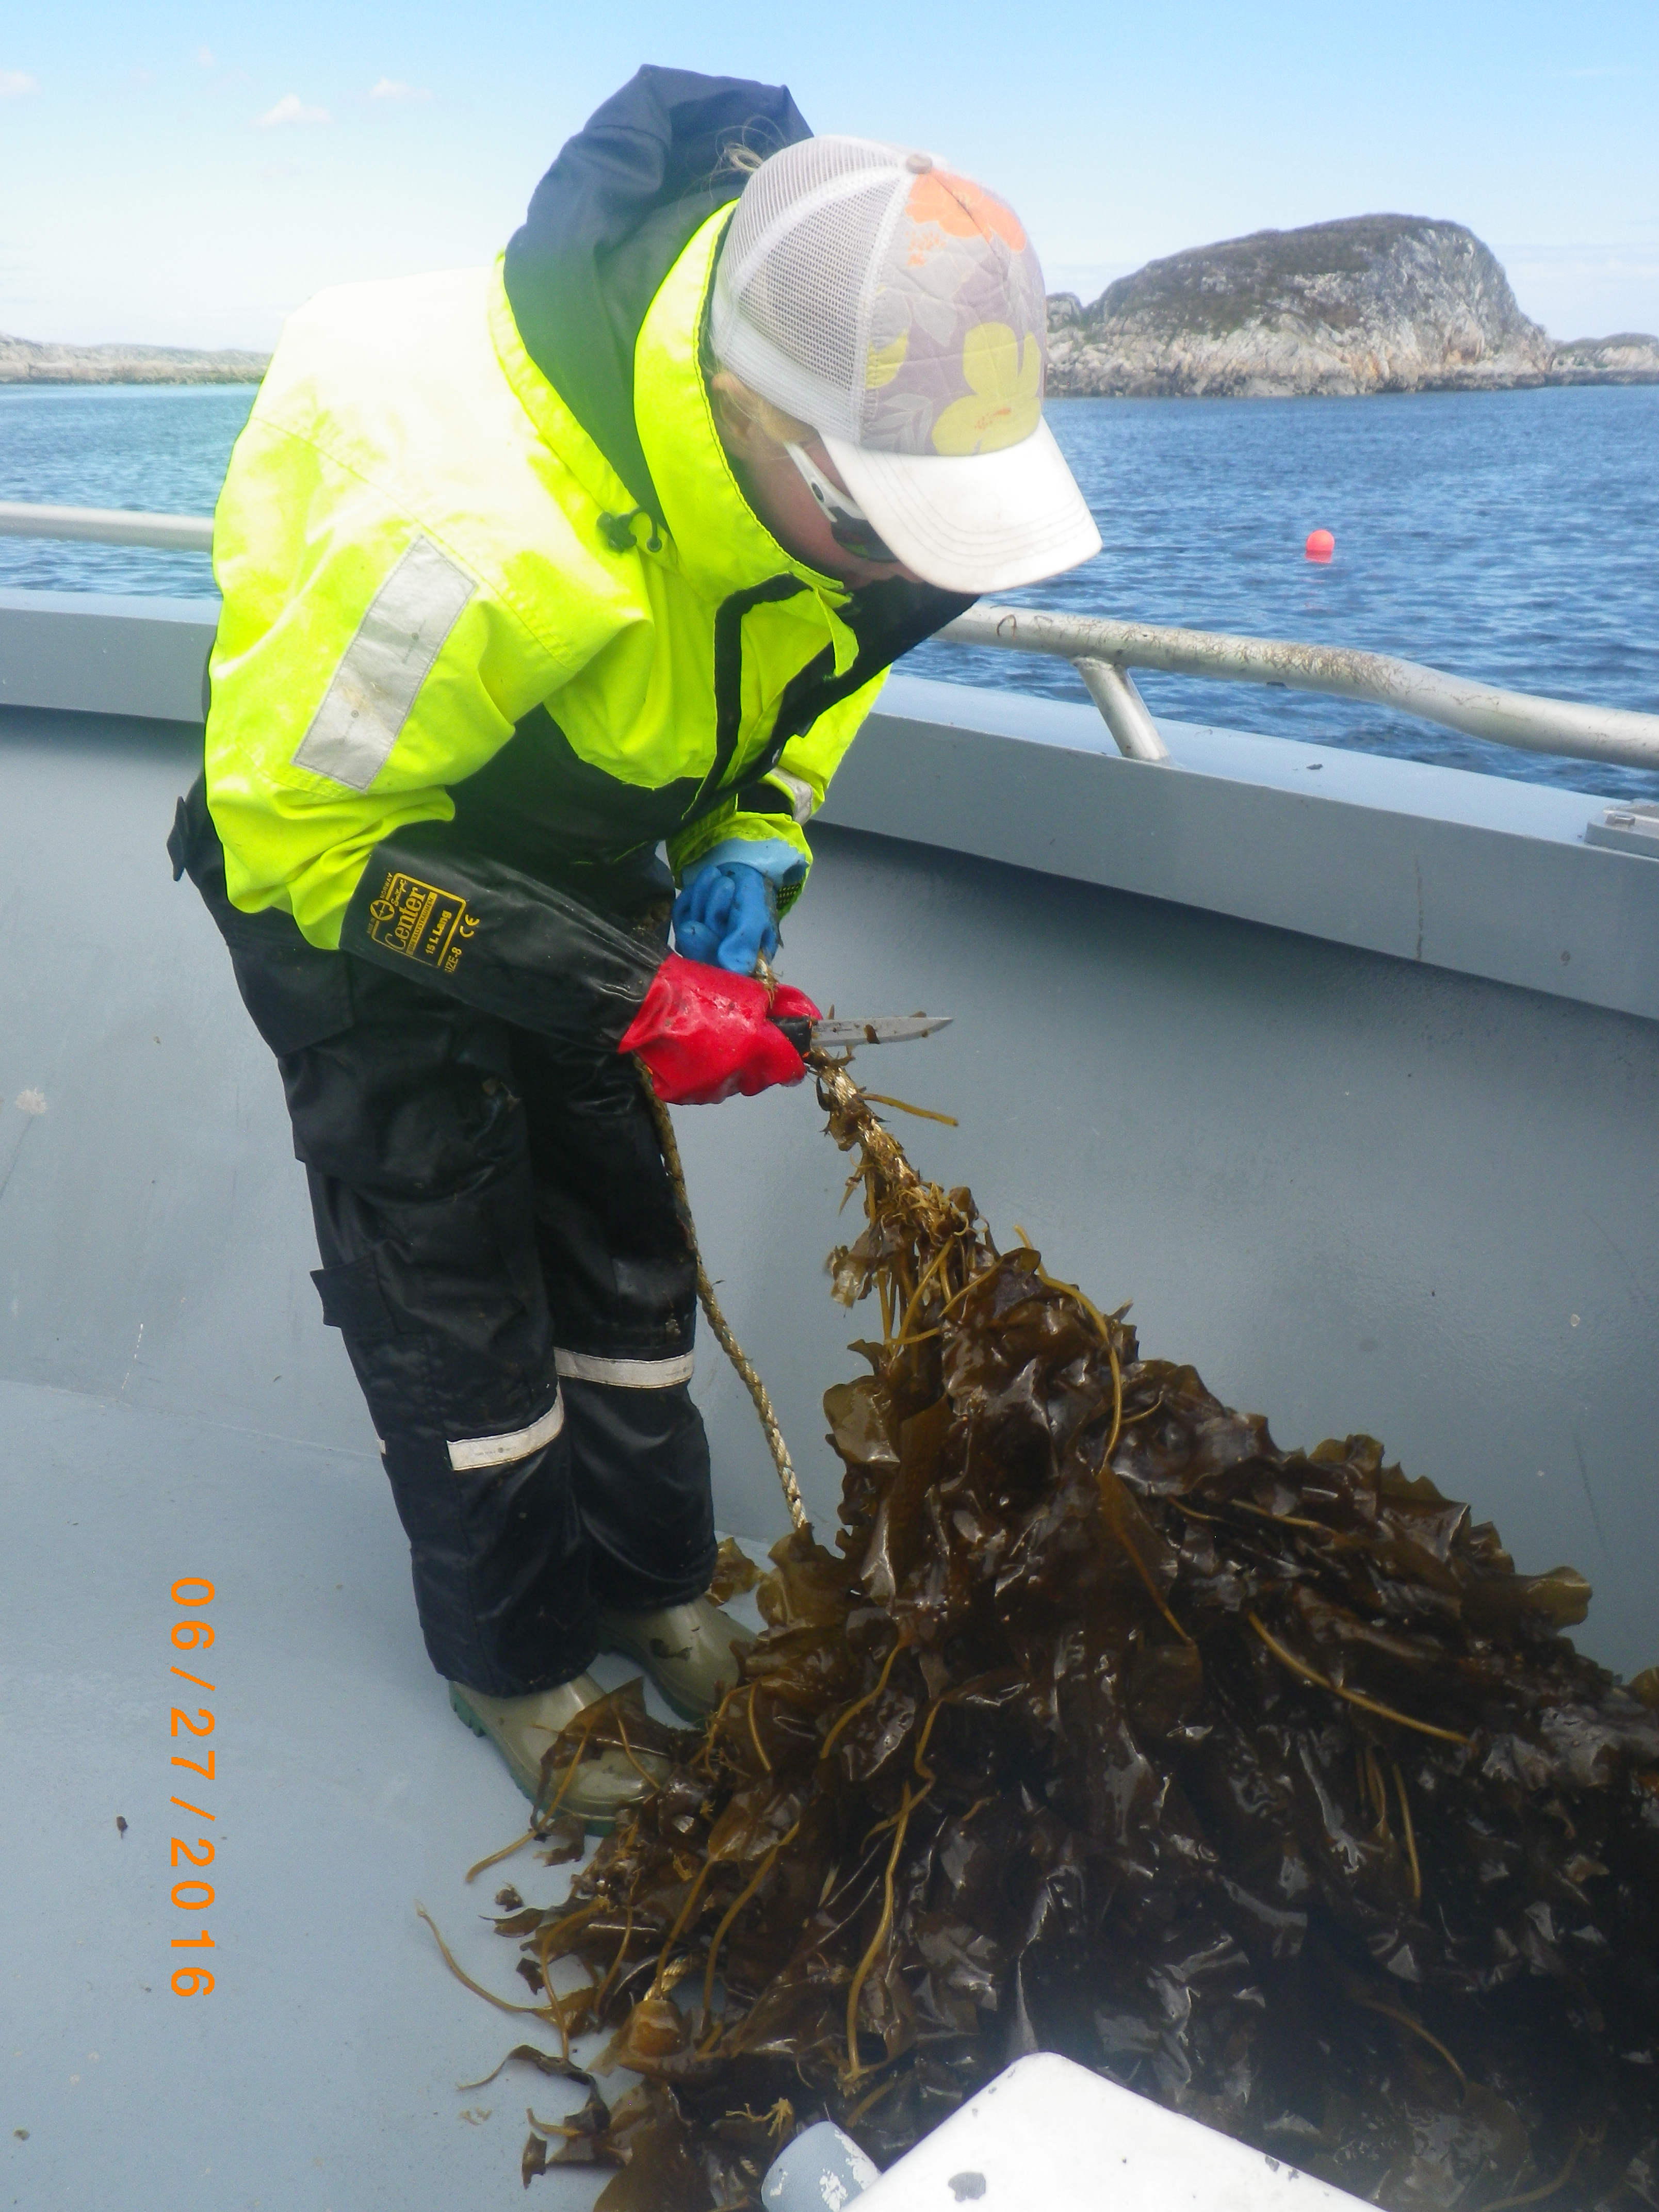
\includegraphics[width=0.5\textwidth]{kelp_photo/sonja}
  \caption{\textit{Saccharina latissima} being harvested}
  \label{fig:sonja}
\end{figure}

Large scale macroalgae cultivation has long existed in Eastern Asia due to the popularity of seaweed in Asian cuisine, and low labor costs that facilitate its manual seeding and harvest.
  More recently, less labor-intense and more industrialized kelp aquaculture has been developing in Scandinavia and in the Northeastern United States and Canada.
  For example, the MACROSEA project is a four year international research collaboration led by SINTEF, an independent research organization in Norway, and funded by the Research Council of Norway.
  The project's aim is to achieve ``successful and predictable production of high quality biomass thereby making significant steps towards industrial macroalgae cultivation in Norway''.
Figure \ref{fig:sonja} shows seaweed being harvested onboard a SINTEF research vessel.
The project includes both cultivators and scientists, working to develop a precise understanding of the full life cycle of kelp and its interaction with its environment.

A fundamental aspect of this endeavor is the development of mathematical models to describe the growth of kelp.
The development of mathematical models enables insight into a system which would be otherwise difficult or impossible to obtain.
For example, imagine that a company is interested in a new IMTA site, and is looking for a suitable location.
Running simulations to predict the potential productivity of each area would be of great assistance in choosing the best site.
Similarly, if a new cultivation technique is under consideration, simulation can estimate its viability without
having to deploy it on a large scale and risk failure or avoidable inefficiency.

Recently, a growth model \cite{broch_modelling_2012} for \textit{S. latissima} has been produced and integrated into the SINMOD \cite{wassmann_modelling_2006} hydrodynamic and ecosystem model of SINTEF.
This kelp model considers factors such as temperature, nutrient concentration, light availability, and water current.
The amount of light available is informed by spatially varying attenuation coefficients from SINMOD,
which considers optical properties of the water as well as concentrations of various organic and inorganic constituents.
However, it does not consider the effect of the kelp itself on the light field.
This is an important consideration, as high kelp densities should lead to low light levels which would inhibit further growth.
However, without accounting for self-shading, the kelp is not adequately penalized for growing too densely,
which is expected to cause overpredictions in the total biomass production.
The purpose of this thesis is to develop a first principles light model which adequately predicts the effects of self-shading on seaweed.


\section{Background on Kelp Models}

Mathematical modeling of macroalgae growth is not a new topic, although it is a reemerging one.
Several authors in the second half of the twentieth century were interested in describing the growth and composition of the macroalgae \textit{Macrocystis pyrifera}, commonly known as ``giant kelp,'' which grows prolifically off the coast of southern California.
The first such mathematical model was developed by W.J. North for the Kelp Habitat Improvement Project at the California Institute of Technology in 1968 using seven variables.
By 1974, Nick Anderson greatly expanded on North's work, and created the first comprehensive model of kelp growth which he programmed using FORTRAN \cite{anderson_mathematical_1974}.
In his model, he accounts for solar radiation intensity as a function of time of year and time of day, and refraction on the surface of the water.
He uses a simple model for shading, specifying a single parameter which determines the percentage of light that is allowed to pass through the kelp canopy floating on the surface of the water.
He also accounts for attenuation due to turbidity using Beer's Law.
Using this data on the availability of light, he calculates the photosynthesis rates and the growth experienced by the kelp.

Over a decade later in 1987, G.A.
Jackson expanded on Anderson's model for \textit{Macrocystis pyrifera} \cite{jackson_modelling_1987}, with an emphasis on including more environmental parameters and a more complete description of the growth and decay of the kelp.
The author takes into account respiration, frond decay, and sub-canopy light attenuation due to self-shading.
Light attenuation is represented with a simple exponential model, and self-shading appears as an added term in the decay coefficient.
The author does not consider radial or angular dependence on shading.
Jackson also expands Anderson's definition of canopy shading, treating the canopy not as a single layer, but as 0, 1, or 2 discrete layers, each composed of individual fronds.
While this is a significant improvement over Anderson's light model, it is still rather simplistic.

Both Anderson's and Jackson's model were carried out by numerically solving a system of differential equations over small time intervals.
In 1990, M.A. Burgman and V.A. Gerard developed a stochastic population model \cite{burgman_stage-structured_1990}.
This approach functions by dividing kelp plants into groups based on size and age and generating random numbers to determine how the population distribution over these groups changes over time based on measured rates of growth, death, decay, light availability, etc.
In the same year, Nyman et. al. \cite{nyman_macrocystis_1990} published a similar model alongside a Markov chain model, and compared the results with experimental data collected in New Zealand.

In 1996 and 1998 respectively, P. Duarte and J.G. Ferreira used the size-class approach to create a more general model of macroalgae growth, and Yoshimori et. al. created a differential equation model of \textit{Laminaria religiosa} with specific emphasis on temperature dependence of growth rate \cite{duarte_model_1997,yoshimori_mathematical_1998}.
These were some of the first models of kelp growth that did not specifically relate to \textit{Macrocystis pyrifera} (``giant kelp'').

The model developed by Broch et. al. at SINTEF \cite{broch_modelling_2012, broch_modelling_2013, handa_seasonal_2013} uses a super-individual approach, whereby a small number of individual kelp fronds are explicitly simulated at several discrete depth layers.
Each super-individual is assumed to represent a certain number of actual individuals in the population.
The number of individuals represented by each super-individual may change over the course of the simulation due to population loss.
The super-individual approach has the advantage of capturing some of the dynamics at the individual scale, while compromising full detail for the sake of reduced computational cost.

\section{Background on Radiative Transfer}
In terms of optical quantities, of primary interest is the radiance, which describes the rate of energy flow through each point in space in \textit{each} direction.
Irradiance, on the other hand, describes the total energy flow through a point in space over \textit{every} direction, and is calculated by integrating radiance over all angles.
Irradiance, in turn, determines the photosynthetic rate of the kelp, and therefore the total amount of biomass producible in a given area as well as the total nutrient remediation potential.
The equation governing the radiance throughout the system is known as the radiative transfer equation (RTE), which has been used extensively in stellar astrophysics \cite{chandrasekhar_radiative_1960,petkova_novel_2011}; its application to marine biology is fairly recent \cite{mobley_radiative_2001}.
In its full form, radiance is a function of 3 spatial dimensions, 2 angular dimensions, and frequency, making for a formidable problem.
In this work, frequency is ignored; only the total radiation in the photosynthetic spectrum, known as photosynthetically active radiation (PAR), is considered.
The RTE states that along a given path, radiance is decreased by absorption and scattering out of the path, while it is increased by emission and scattering into the path.
In the case of macroalgae cultivation, emission is negligible, owing only perhaps to some small luminescent phytoplankton or other anomaly, and can therefore be safely ignored.
However, the emission term will be retained in the calculations of this thesis, as it is mathematically useful to verify the correctness of the solution algorithm.

\section{Overview of Thesis}
The remainder of this document is organized as follows.
In Chapter II, a probabilistic model is developed to describe the spatial distribution of kelp by assuming simple distributions for the lengths and orientations of fronds.
Chapter III begins with a survey of fundamental radiometric quantities and optical properties of matter.
The spatial kelp distribution from Chapter II is used to determine optical properties of the combined water-kelp medium,
and the radiative transfer equation, an integro-partial differential equation which describes the the light field as a function of position and angle, is discussed.
An asymptotic expansion is explored for the case of low scattering, allowing for analytical, ordered approximations to the true light field.
In Chapter IV, details are given for the numerical solution of the equations from Chapters II and III.
Both the full finite difference solution and the asymptotic approximation are thoroughly developed.

Chapter V is an in--depth discussion of sources of error in both solution procedures.
The concepts of verifying codes in general as well as specific calculations are discussed.
Exact discretization errors are calculated via the method of manufactured solutions in order to demonstrate
that the methods exhibit convergence properties which build confidence in their correctness.
A method for estimating errors for realistic cases is also developed.

Next, Chapter VI surveys practical considerations to keep in mind when applying the algorithms in real situations.
Relevant model parameter values from the literature are collected, and estimates are given for those not readily available.
Following that is a set of guidelines for choosing which algorithm and which algorithm parameters to use based on the optical scenario to be simulated.
Advantages and disadvantages of both approaches are presented.
While the finite difference technique can be applied to any situation, it often requires prohibitively large CPU and memory resources, whereas the numerical asymptotic solution is generally faster and its memory footprint never exceeds the capacity of a standard laptop for reasonable grid sizes.
The Chapter concludes with a comparison to other two simpler light models, and specific qualitative differences are noted.
As expected, the presence of self-shading in this model results in the prediction of lower light levels regions of high kelp density.
However, the presence of scattering in the model increases light levels elsewhere, especially near the surface of the water.

Finally, Chapter VII concludes the thesis by briefly summarizing the model, discussing its achievements and limitations, and suggesting improvements and avenues for future work.
Several appendices follow with further details about the algorithm, as well as the full source code of the Fortran model developed.

\chapter{KELP MODEL}
\label{chap:kelp}

In order to properly model the spatial distribution of light around the kelp, it is first necessary to formulate a spatial description of the kelp.
Probability distributions are given for the size and orientation of the individual kelp fronds, which are inverted to determine the probability of a point in space being occupied by kelp.
Ultimately, the kelp density at any point in space is calculated, which informs the absorption coefficient of the effective kelp--water medium.


\section{Physical Setup}
The life of cultivated macroalgae generally begins in the laboratory, where microscopic kelp spores are inoculated onto a thread in a small laboratory pool.
This thread is wrapped around a larger rope as in Figure \ref{fig:rope_thread}, which is hung from buoys in the ocean.
The two primary configurations are vertical and horizontal or ``long'' lines.
In the case of vertical lines, the seaweed rope hangs straight down from a single buoy, and is either weighted or anchored.
In the case of long lines, the rope is strung from one buoy to another.
Long lines allow more light to reach the seaweed since it grows closer to the surface, but more vertical lines can be set up in a given area,
which may be advantageous for IMTA.

\begin{figure}[H]
  \centering
  \includegraphics[width=0.65\textwidth]{kelp_photo/rope_thread}
  \caption{\textit{Saccharina latissima} innoculated onto a thread wrapped around a rope on which it is to be grown.}
  \label{fig:rope_thread}
\end{figure}

We consider only the case of a rigid vertical rope which does not sway in the current.
The mature \textit{Saccharina latissima} plant consists of a single frond (leaf), a stipe (stem) and a holdfast (root structure).
For the sake of this model, only the kelp frond is considered, and its base is attached directly to the rope.
The ``gentle undulation approximation'' is employed, whereby the fronds are modeled as perfectly horizontal.
While at any given time they may point up or down due to water current and gravity, we consider the horizontal
state to be an average configuration.
This simplification allows for the three-dimensionally distributed population of kelp fronds
to be considered a collection of independent populations in two-dimensional depth layers.
A computer rendering of this scenario is shown in Figure \ref{fig:kelp_array}.

\begin{figure}[H]
	\centering
	\includegraphics[width=3.5in]{kelp_array}
	\captionof{figure}{Rendering of four nearby vertical kelp ropes as represented in the spatial distribution model. Note the kite--shaped fronds and horizontal orientation.}
  \label{fig:kelp_array}
\end{figure}

\section{Coordinate System}
Consider the rectangular domain
\begin{align*}
  \xmin &\leq x \leq \xmax, \\
  \ymin &\leq y \leq \ymax, \\
  \zmin &\leq z \leq \zmax.
\end{align*}
For all three dimensional analysis, we use the absolute coordinate system defined in Figure \ref{fig:3dcoords}.
In the following sections, it is necessary to convert between Cartesian and spherical coordinates, which we do using the relations
\begin{equation}
  \left\{
	\begin{split}
		x & = r\sin\phi\cos\theta, \\
		y & = r\sin\phi\sin\theta, \\
		z & = r\cos\phi. \\
	\end{split}
  \right.
	\label{eqn:coords}
\end{equation}
Therefore, for some function $f(x,y,z)$, we can write its derivative along a path in spherical coordinates in terms of Cartesian coordinates using the chain rule,
\begin{equation*}
	\frac{\partial f}{\partial r}
	=\frac{\partial f}{\partial x}\frac{\partial x}{\partial r}
	+ \frac{\partial f}{\partial y}\frac{\partial y}{\partial r}
	+ \frac{\partial f}{\partial z}\frac{\partial z}{\partial r}.
\end{equation*}
Then, calculating derivatives from \eqref{eqn:coords} yields
\begin{equation}
	\frac{\partial f}{\partial r}
	=\frac{\partial f}{\partial x}\sin\phi\cos\theta
	+ \frac{\partial f}{\partial y}\sin\phi\sin\theta
	+ \frac{\partial f}{\partial z}\cos\phi.
	\label{eqn:partials}
\end{equation}
\begin{figure}[H]
	\centering
	\includegraphics[width=3in]{3d_coords}
	\caption{Downward-facing right-handed coordinate system with radial distance $r$ from the origin, distance $s$ from the $z$ axis, zenith angle $\phi$ and azimuthal angle $\theta$.}
	\label{fig:3dcoords}
\end{figure}

\section{Population Distributions}
In order to construct a spatial distribution of kelp fronds, a simple kite-shaped geometry is introduced,
and frond lengths and azimuthal orientations are assumed to be distributed predictably.
Since it is assumed that fronds extend perfectly horizontally, no angular elevation distribution is required.

\subsection{Frond Shape}
\label{sec:shape}

\begin{figure}[h]
	\centering
  \includegraphics[width=1.2in]{kelp_photo/kite}
  %TODO: Cite this?
  \qquad
	\includegraphics[width=2in]{frond}
	\captionof{figure}{Simplified kite-shaped frond.}
	\label{fig:frond}
\end{figure}

The frond is assumed to be kite-shaped with length $l$ from base to tip, and width $w$ from left to right.
In Figure \ref{fig:frond}, the base is shown at the bottom and the tip is shown at the top.
The proximal length is the shortest distance from the base to the diagonal connecting the left and right corners, and is notated as $f_a$.
Likewise, the distal length, notated $f_b$, is the shortest distance from that diagonal to the tip.
It is therefore clear that
 \begin{equation*}
	 f_a + f_b = l.
 \end{equation*}
When considering a whole population with varying sizes, it is more convenient to specify ratios than absolute lengths.
Define the ratios
\begin{align*}
	f_r &= \frac{l}{w}, \\
	f_s &= \frac{f_a}{f_b}.
\end{align*}
These ratios are assumed to be constant among the entire population, so that all fronds are geometrically similar.
Thus, the shape of the frond can be fully specified by $l$, $f_r$, and $f_s$;
it is possible to redefine $w$, $f_a$ and $f_b$ from the preceding formulas as
\begin{align*}
	w &= \frac{l}{f_r}, \\
	f_a &= \frac{lf_s}{1+f_s}, \\
	f_b &= \frac{l}{1+f_s}.
\end{align*}
The angle $\alpha$, half of the angle at the base corner, is also noteworthy.
From the above equations, it follows that
\begin{equation*}
	\alpha = \tan^{-1}\left(\frac{2f_rf_s}{1+f_s}\right).
\end{equation*}

It is useful to convert between frond length and surface area, which can be done via the relations
\begin{align}
  A &= \frac{lw}{2} = \frac{l^2}{2f_r},
  \DIFdelbegin %DIFDELCMD < \label{eqn:area-from-length} %%%
\DIFdelend \DIFaddbegin \label{eqn:area_from_length} \DIFaddend \\
  l &= \sqrt{2Af_r}.
  \DIFdelbegin %DIFDELCMD < \label{eqn:length-from-area}
%DIFDELCMD < %%%
\DIFdelend \DIFaddbegin \label{eqn:length_from_area}
\DIFaddend \end{align}

\subsection{Length and Angle Distributions}
\label{sec:dist}
In any given depth layer, the distribution of frond lengths is assumed to be normal, with mean $\mu_l$ and standard deviation $\sigma_l$.
That is, it has the probability density function (PDF)
\begin{equation*}
  P_l(l) = \frac{1}{\sqrt{2\pi\sigma_l^2}}\exp\left(-\frac{(l-\mu_l)^2}{2\sigma_l^2}\right).
\end{equation*}

It is further assumed that frond orientation angle varies according to the von Mises distribution, which is the periodic analogue of the normal distribution, defined on $[-\pi,\pi]$ rather than $(-\infty,\infty)$.
The von Mises distribution has two parameters, $\mu$ and $\kappa$, which shift and sharpen its peak respectively, as shown in Figure \ref{fig:vonmises}.
$\kappa$ is analogous to $1/\sigma$ in the normal distribution.
In the absence of current, the frond angles are distributed uniformly, while as current velocity increases, they become increasingly likely to align parallel to the current, depending on the stiffness of the frond and stipe.
Assuming a linear relationship between the current velocity and the steepness of the angular distribution, define the \textit{frond alignment coefficient} $\eta$, with units of inverse velocity(\SI{}{\s\per\m}).
Then, use $\mu = \theta_w$ and $\kappa = \eta v_w$ as the von Mises distribution parameters.
Note that $\theta_w$ and $v_w$ vary over depth, while $\eta$ is assumed constant for the population.
Then, the PDF for the von Mises frond angle distribution is
\begin{equation*}
	P_{\theta_f}(\theta_f) = \frac{\exp\left(\eta v_w\cos(\theta_f-\theta_w)\right)}{2\pi I_0(\eta v_w)},
\end{equation*}
where $I_0(x)$ is the modified Bessel function of the first kind of order 0.
Notice that unlike the normal distribution, the von Mises distribution approaches a \textit{non-zero} uniform distribution as $\kappa$ approaches 0, so
\begin{equation*}
	\displaystyle \lim_{v_w \to 0}P_{\theta_f}(\theta_f) = \frac{1}{2\pi} \;\forall\, \theta_f \in [-\pi,\pi].
\end{equation*}

\begin{figure}[h]
	\centering
	\includegraphics[width=6in]{vonmises}
	\captionof{figure}{von Mises distribution for a variety of parameters.}
	\label{fig:vonmises}
\end{figure}

\subsection{Joint Length-Orientation Distribution}
\label{sec:dist_2d}
The previous two distributions can reasonably be assumed to be independent of one another. That is, the angle of the frond does not depend on the length, or vice versa.
Therefore, the probability of a frond simultaneously having a given frond length and angle is the product of their individual probabilities.
Given independent events $A$ and $B$, the probability of their intersection is the product of their individual probabilities.
That is,
\begin{equation*}
	\label{eqn:ind_prob}
	P(A \cap B) = P(A)P(B).
\end{equation*}
Then the probability of frond length $l$ and frond angle $\theta_f$ coinciding is
\begin{equation}
  \label{eqn:p2d}
	P_{2D}(\theta_f,l) = P_{\theta_f}(\theta_f) \cdot P_l(l).
\end{equation}
A contour plot of this 2D distribution for a specific set of parameters is shown in Figure \ref{fig:dist_2d}, where probability is represented by color in the 2D plane.
Darker green represents higher probability, while lighter beige represents lower probability.
In Figure \ref{fig:kelp_sample}, 50 samples are drawn from this distribution and plotted.

It is important to note that if $P_{\theta_f}$ were dependent on $l$, the above definition of $P_{2D}$ would no longer be valid.
For example, it might be more realistic to say that larger fronds are less likely to bend towards the direction of the current.
In this case, \eqref{eqn:ind_prob} would no longer hold, and it would be necessary to use the more general Bayes' Theorem
\begin{equation*}
	P(A \cap B) = P(A)P(B|A) = P(B)P(B|A),
\end{equation*}
which is currently not taken into consideration in this model.

\begin{figure}[h]
	\centering
	\includegraphics[width=4.5in]{prob_2d}
	\captionof{figure}{2D length-angle probability distribution with $\theta_w=7\pi/4$, $v_w=1$, $\mu_l=3$, $\sigma_l=1$.}
	\label{fig:dist_2d}
\end{figure}

\begin{figure}[h]
	\centering
	\includegraphics[width=4.5in]{kelp_sample}
	\captionof{figure}{A sample of 50 kelp fronds with shape parameters $f_s=0.5$ and $f_r=2$ whose lengths are picked from a normal distribution and whose angles are picked from a von Mises distribution.}
	\label{fig:kelp_sample}
\end{figure}

\section{Spatial Distribution}
In this section, the population length and angle distributions from the previous section are used to construct a spatial distribution of kelp.
This is made possible by the simple kite-shape fronds, and would be considerably more difficult with more general frond shapes.
\subsection{Rotated Coordinate System}
\label{sec:rot_coords}
To determine under what conditions a frond will occupy a given point, we begin by
describing the shape of the frond in Cartesian coordinates and then convert to polar coordinates.
Of primary interest are the edges connected to the frond tip.
For convenience, we will use a rotated polar coordinate system $(\theta',s)$ such that the line connecting the base to the tip points in the $+y$ direction ($\theta=\pi/2$), with the base at $(0,0)$.
Denote the Cartesian analogue of this coordinate system as $(x',y')$ which is related to $(\theta',s)$ by
\begin{align*}
	x' &= s\cos\theta' \\
	y' &= s\sin\theta' \\
	s &= \sqrt{x'^2+y'^2}, \\
	\theta' &= \atantwo(y, x).
\end{align*}

\subsection{Functional Description of Frond Edge}
With this coordinate system established, the outer two edges of the frond can be described in Cartesian coordinates as a piecewise linear function connecting the left corner: $(-w/2,f_a)$, the tip: $(0,l)$, and the right corner: $(w/2,f_a)$.
This function has the form
\begin{equation*}
	y'_f(x') = l-\sign(x')\frac{f_b}{w/2}x'.
\end{equation*}
Using the equations in Section \ref{sec:rot_coords}, this can be written in polar coordinates after some rearrangement as
\begin{equation*}
	s_f'(\theta';l) = \frac{l}{\sin\theta' + S(\theta')\frac{2f_b}{w}\cos\theta'},
\end{equation*}
where
\begin{equation*}
	S(\theta') = \sign(\cos\theta').
\end{equation*}
Then, using the relationships in Section \ref{sec:shape}, the above equation can be rewritten in terms of the frond ratios $f_s$ and $f_r$ as
\begin{equation}
	\label{eqn:rf_rel}
	s_f'(\theta';l) = \frac{l}{\sin\theta' + S(\theta')\frac{2f_r}{1+f_s}\cos\theta'}.
\end{equation}
For convenience, denote the denominator of \eqref{eqn:rf_rel} as $d_f'(\theta')$.
To generalize to a frond pointed at an angle $\theta_f$, we introduce the coordinate system $(\theta,s)$ such that
\begin{equation*}
	\theta = \theta' + \theta_f - \frac{\pi}{2}.
\end{equation*}
Then, for a frond pointed at the arbitrary angle $\theta_f$, the function for the outer edges can be written as
\begin{equation}
	\label{eqn:rf_abs}
	s_f(\theta;l) = s_f'\left(\theta - \theta_f + \frac{\pi}{2} \right).
\end{equation}
Similarly, define
\begin{equation}
	d_f(\theta) = d_f'\left(\theta - \theta_f + \frac{\pi}{2} \right).
\end{equation}

\subsection{Conditions for Occupancy}
We now formulate the conditions under which a kite shape frond occupies a point
in the sense that the point lies within its interior.
Combining these conditions with the size and orientation distributions from \ref{sec:dist}
allows a spatial distribution of the kelp fronds to be calculated.

Consider a fixed frond of length $l$ at an angle $\theta_f$. The point
$(\theta,s)$ is occupied by the frond if
\begin{align*}
	\left|\theta_f - \theta \right| < \alpha
  \mbox{ and }
	s < s_f(\theta).
\end{align*}
Equivalently, the opposite perspective can be taken.
Letting the point $(\theta,s)$ be fixed, a frond occupies the point if
\begin{align}
	\theta - \alpha < \theta_f < \theta + \alpha,
	\label{eqn:rs_th} \\
	l > l_{\min}(\theta,s),
	\label{eqn:rs_l}
\end{align}
where
\begin{equation}
	l_{\min}(\theta,s) = s \cdot \frac{l}{s_f(\theta;l)} = s \cdot d_f(\theta).
  \label{eqn:l_min}
\end{equation}
Then, considering the point to be fixed, \eqref{eqn:rs_th} and \eqref{eqn:rs_l} define the spacial region $R_s(\theta,s)$ called the ``occupancy region for $(\theta,s)$'' with the property that if the tip of a frond lies within this region (i.e., $(\theta_f,l) \in R_s(\theta,s)$), then it occupies the point.
$R_s(3\pi/4,1.5)$ is shown in blue in Figure \ref{fig:shade_area} and the smallest possible occupying fronds for several values of $\theta_f$ are shown in various colors.
Any frond longer than these at the same angle will also occupy the point.

\begin{figure}[h]
	\centering
	\includegraphics[width=4.5in]{shade_area}
	\captionof{figure}{Outlines of minimum-length fronds for a variety of angles to occupy the point $(\theta,s)=(3\pi/4,3/2)$.}
	\label{fig:shade_area}
\end{figure}

\subsection{Probability of Occupancy}
We are interested in the probability that, given a fixed point $(\theta,s)$, values of $l$ and $\theta_f$ chosen from the distributions described in Section \ref{sec:dist} will fall in the occupancy region.
This is found by integrating $P_{2D}(\theta_f, l)$ from \eqref{eqn:p2d} over $R_s(\theta,s)$, the occupancy region for the point of interest.

\begin{figure}[h]
	\centering
	\includegraphics[width=4.5in]{cart_shade}
	\captionof{figure}{Contour plot of $P_{2D}(\theta_f,l)$ overlayed with the
    region in the $\theta_f$\nobreak--\nobreak$l$ plane which results in a frond occupying the point $(\theta,s)=(3\pi/4,3/2)$.}
	\label{fig:cart_shade}
\end{figure}

Integrating $P_{2D}(\theta_f,l)$ over $R_s(\theta,s)$ as depicted in Figure \ref{fig:cart_shade} yields the proportion of the population in the depth layer occupying the point $(\theta,s)$,
\DIFdelbegin \begin{align*}
		\DIFdel{\tilde{P}_k(\theta,s,z)	}&\DIFdel{= \iint_{R_s(\theta,s)}
								P_{2D}(\theta_f,l)
								\,dl\,d\theta_f \nonumber }\\
							&\DIFdel{= \int_{\theta-\alpha}^{\theta+\alpha}
								\int_{l_{\min}(\theta_f)}^\infty
								P_{2D}(\theta_f,l)
								\,dl\,d\theta_f.
}\end{align*}
%DIFAUXCMD
\DIFdelend \DIFaddbegin \begin{align}
		\DIFadd{\tilde{P}_k(\theta,s,z)	}&\DIFadd{= \iint_{R_s(\theta,s)}
								P_{2D}(\theta_f,l)
								\,dl\,d\theta_f \nonumber }\\
							&\DIFadd{= \int_{\theta-\alpha}^{\theta+\alpha}
								\int_{l_{\min}(\theta_f)}^\infty
								P_{2D}(\theta_f,l)
								\,dl\,d\theta_f.
                \label{eqn:integrate_p2d}
}\end{align}
\DIFaddend 

Assuming that the depth layer has thickness $dz$ and contains \DIFdelbegin \DIFdel{$n$ }\DIFdelend \DIFaddbegin \DIFadd{$n_f$ }\DIFaddend fronds of thickness \DIFdelbegin \DIFdel{$t$}\DIFdelend \DIFaddbegin \DIFadd{$f_t$}\DIFaddend ,
the proportion of the vertical length of the discrete depth layer occupied by kelp at any position $(x,y,z)$ is given by
\DIFdelbegin \begin{displaymath}
  \DIFdel{P_k(x, y) = \frac{nt}{dz}\tilde{P}_k(x, y).
}\end{displaymath}
%DIFAUXCMD
\DIFdelend \DIFaddbegin \begin{equation}
  \DIFadd{P_k(x, y) = \frac{n_ff_t}{dz}\tilde{P}_k(x, y).
  \label{eqn:kelp_pk}
}\end{equation}
\DIFaddend In the continuum limit as the number of discrete depth depth layers approaches infinity, $P_k(x,y,z)$ can be interpreted as the probability of the point $(x,y,z)$ being occupied by kelp.
In a three dimensional context, the number of fronds is more likely to be specified by a number density \DIFdelbegin \DIFdel{$\rho_n=n/dz$ }\DIFdelend \DIFaddbegin \DIFadd{$\rho_f=n_f/dz$ }\DIFaddend over the vertical length of the rope with units \SI{}{\per\m}, in which case
\DIFdelbegin \begin{displaymath}
  \DIFdel{P_k(x, y, z) = t \rho_n(z) \tilde{P}_k(x, y, z).
}\end{displaymath}
%DIFAUXCMD
\DIFdelend \DIFaddbegin \begin{equation}
  \DIFadd{P_k(x, y, z) = f_t \rho_f(z) \tilde{P}_k(x, y, z).
}\end{equation}
\DIFaddend Then, since the point $\vec{x}$ has a probability $P_k(\vec{x})$ of being occupied by kelp and a probability $(1-P_k(\vec{x}))$ of being occupied by the surrounding aquatic medium,
the effective absorption coefficient can be calculated as
\begin{equation*}
  \DIFaddbegin \label{eqn:abs_field}
  \DIFaddend a(\vec{x}) = P_k(\vec{x})a_k + (1-P_k(\vec{x}))a_w,
\end{equation*}
where $a_k$ is the absorption coefficient of the kelp alone, and $a_w$ is the absorption coefficient of the water and its dissolved and suspended contents.

\begin{figure}[h]
	\centering
	\includegraphics[width=4.5in]{prob_shade}
	\captionof{figure}{Contour plot of the probability of frond occupation sampled at 121 points using $\theta_f=2\pi/3,\eta v_w=1$.}
	\label{fig:prob_shade}
\end{figure}

\section{Discontinuity at the rope}
While the above model of the kelp distribution is straightforward to evaluate, it does have a significant numerical difficulty in its application.
Since the length and orientations are both continuous in the polar coordinates $s>0$ and $\theta$, the resulting kelp density and effective absorption coefficient are as well.
However, they are not necessarily continuous in Cartesian coordinates.
In the case of no water current, $v_w=0$, the flat von Mises distribution produces a continuous solution at the origin.
In the more general case, though, there is a high kelp density on one side of the origin in the direction of the current, and a low kelp density immediately on the other side.
Since the rope is assumed to be infinitely thin and have a fixed position, the sharp corners of the kelp fronds emanate from exactly the same point.
Hence, there is in general a discontinuity in the kelp distribution at the origin, and therefore its derivatives are unbounded on the domain.

This is not appealing numerically since the algorithms used in this thesis to solve the differential equation describing the light field are based on interpolation on a discrete Cartesian grid.
According to Taylor's theorem, the error incurred by performing such interpolation is bounded by a constant multiple of the appropriate maximum derivative of the interpolated function over the domain.
If the derivatives of the absorption coefficient are unbounded, then so too is the discretization error in the final solution.
That is, the solution is not guaranteed to converge.

Luckily, there is a straightforward solution, which is to post-process the spatial kelp distribution with a Gaussian blur in the $x$ and $y$ dimensions.
This is achieved via convolution of the solution with a 2D Gaussian kernel centered at the origin.
Any blur whatsoever is sufficient to bound the derivatives, and the larger the blur radius, the smaller they become.
Obviously, as the blur radius is increased, the kelp distribution tends toward a constant and no longer captures any information about the $xy$ distribution of the kelp.
Therefore, a small blur radius should be used.

\subsection{One dimensional Gaussian blur}
As a one dimensional analogy, consider the Heaviside step function,
\begin{equation*}
  H(x) = \begin{cases}
    0, & x < 0, \\
    1, & x > 0.
  \end{cases}
\end{equation*}
Clearly, the function is infinitely steep at the origin.
Consider the normalized Gaussian kernel centered at the origin with radius $\sigma_b$, given by
\begin{equation}
  k(x;\sigma_b) = \DIFdelbegin \DIFdel{\frac{1}{\sqrt{2\pi\sigma_b}^2} }\DIFdelend \DIFaddbegin \DIFadd{\frac{1}{\sqrt{2\pi\sigma_b^2}} }\DIFaddend \exp\left({-\frac{x^2}{2\sigma_b^2}}\right).
\end{equation}
A blur is applied by convolving the function with the kernel according to the formula
\begin{align*}
  \tilde{H}(x) &= (k*H)(x) = \int_{-\infty}^{\infty}H(\tau)k(x-\tau;\sigma_b)\, d\tau \\
  &= \int_{0}^{\infty}k(x-\tau;\sigma_b)\, d\tau.
\end{align*}
The substitution $u=\tau=x,\, du=d\tau$ yields
\begin{equation*}
  \tilde{H}(x) = \int_{-x}^\infty k(u;\sigma_b)\, du.
\end{equation*}
Note that since the kernel is normalized, the integral from 0 to infinity is $1/2$.
Further, since the kernel is even, the integral over $[-x, 0]$ is equal to the integral over $[0, x]$.
Hence,
\begin{equation*}
  \tilde{H}(x) = \frac{1}{2} + \int_{0}^x k(u;\sigma_b)\, du.
\end{equation*}
Then, by the fundamental theorem of calculus, the derivative of the convolved function is simply $k(x;\sigma_b)$, whose maximum value is $k(0;\sigma_b) = 1/\sqrt{2\pi\sigma_b^2}$.
Then, since the derivative is a linear operator, this result can be generalized to the following statement:
Applying a Gaussian blur of radius $\sigma_b$ to a function with a maximum discontinuity of size $J$ produces a function whose first derivative is bounded by
\begin{equation*}
  \frac{1}{\sqrt{2\pi}}\frac{J}{\sigma_b}.
\end{equation*}
The same logic applies to directional derivatives of multidimensional scalar functions.

\subsection{Multidimensional Gaussian \DIFdelbegin \DIFdel{blur}\DIFdelend \DIFaddbegin \DIFadd{Blur}\DIFaddend }
\DIFaddbegin \label{sec:gaussian_blur}
\DIFaddend In light of the above arguments, the derivatives of the absorption coefficient are bounded by applying a \DIFdelbegin \DIFdel{two--dimensional Gaussian blur in $xy$--plane }\DIFdelend \DIFaddbegin \DIFadd{Gaussian blur }\DIFaddend to $P_k$ \DIFdelbegin \DIFdel{using the kernel
}\DIFdelend \DIFaddbegin \DIFadd{before the calculation of $a(\vec{x})$.
This is done by convolving slices of $P_k$ in the $xy$--plane with the two--dimensional normalized Gaussian kernel
}\DIFaddend \begin{equation}
  \DIFdelbegin \DIFdel{k}\DIFdelend \DIFaddbegin \label{eqn:gaussian_kernel}
  \DIFadd{K}\DIFaddend (x, y; \sigma_b) = \frac{1}{\sqrt{2\pi\sigma_b^2}} \exp\left(\frac{x^2 + y^2}{2\sigma_b^2}\right).
\end{equation}
Hence, the blurred solution is 
\begin{equation}
  \DIFaddbegin \label{eqn:gaussian_blur}
  \DIFaddend P_k^b(x, y, z) = \int_{-\infty}^\infty \int_{-\infty}^\infty \DIFdelbegin \DIFdel{k}\DIFdelend \DIFaddbegin \DIFadd{K}\DIFaddend (\DIFdelbegin \DIFdel{x-x}\DIFdelend \DIFaddbegin \DIFadd{x}\DIFaddend ', \DIFdelbegin \DIFdel{y-y}\DIFdelend \DIFaddbegin \DIFadd{y}\DIFaddend ', z; \sigma_b) P_k(\DIFdelbegin \DIFdel{x}\DIFdelend \DIFaddbegin \DIFadd{x-x}\DIFaddend ', \DIFdelbegin \DIFdel{y}\DIFdelend \DIFaddbegin \DIFadd{y-y}\DIFaddend ', z)\, dx'\, dy'.
\end{equation}

A physical interpretation of this Gaussian blurring is that $P_k^b$ is the time--averaged kelp distribution, assuming that the rope is allowed to move horizontally, and $k(x, y; \sigma)$ is the PDF of the rope's location distribution.
This interpretation is a bit incongruous with the rest of the model since there is no other explicit mention of time--averaging; while the frond length and position distributions can be thought of as continuous approximations to the population distribution at a single point in time, this idea does not apply to the rope's position, since there is only one \DIFaddbegin \DIFadd{rope}\DIFaddend .

\subsection{Absorption coefficient plots}
% TODO: Clean up figures
A variety of numerically calculated absorption coefficient fields are shown here in order to demonstrate some key features of the kelp distribution.
In each figure, the absorption coefficient is plotted on the color axis, while the norm of its gradient is shown with contours, with brighter contour lines representing regions of large derivatives.
As mentioned above, large derivatives generate large discretization error, and are therefore undesirable.
Of course, the distributions must be sufficiently well--defined to capture the characteristics of the kelp.

Figure \ref{fig:kelp_dist_sharp} shows a sharp kelp distribution with an unrealistically high current velocity, with all fronds identically equal in length, and with no blurring applied.
Note the kite--shaped distribution, as expected.
Also note the regions of high derivatives near the origin and inner edges.
This sharp distribution requires excessively large numerical grids to approximate well, and is therefore undesirable.
\begin{figure}[H]
  \centering
  \includegraphics[width=5in]{kelp_dist_sharp}
  \caption{Absorption coefficient profile in the limiting case of $v_w>>1$, $\sigma_l=0$ and $\sigma_b=0$ demonstrates the kite--shaped fronds. Note the high gradient near the inner edge of the frond.}
  \label{fig:kelp_dist_sharp}
\end{figure}

In Figure \ref{fig:kelp_dist_smooth}, the current velocity has been reduced, and a nonzero standard deviation has been given to the frond distribution.
With a variety of frond lengths, the edges are no longer as clearly defined, although the general character of the distribution is sensible --- the kelp is most dense near the rope in the direction of the current.
However, note that there remains a small neighborhood of sharp derivatives encompassing the origin.
Such a distribution would still cause numerical difficulties for the numerical algorithm.

\begin{figure}[H]
  \centering
  \vspace{-3em}
  \includegraphics[width=5in]{kelp_dist_smooth}
  \caption{Absorption coefficient profile for realistic values of $v_w$ and $\sigma_l$, but with $\sigma_b=0$. Note the large gradient at the origin. By continuing to increase the plotting resolution, the gradient would be found to be unbounded.}
  \label{fig:kelp_dist_smooth}
\end{figure}

Figure \ref{fig:kelp_dist_smooth_smallblur} is similar to Figure \ref{fig:kelp_dist_smooth}, except it has been post--processed with a small Gaussian blur of radius \SI{10}{cm}, not so large that it significantly distorts the shape of the distribution, but sufficient to remove the discontinuity in the origin.
Such a kelp distribution is ideal, as it balances accuracy with ease of numerical approximation.
\begin{figure}[H]
  \centering
  \vspace{-3em}
  \includegraphics[width=5in]{kelp_dist_smooth_smallblur}
  \caption{A small blur radius of $\sigma_b=\SI{0.1}{\m}$ eliminates the derivative singularity at the origin.}
  \label{fig:kelp_dist_smooth_smallblur}
\end{figure}

In Figure \ref{fig:kelp_dist_smooth_blur}, too large of a blur has been applied; the character of the Gaussian kernel has overwhelmed that of the kelp distribution.
While this may still provide a better spatial description of the kelp than a fully horizontally uniform distribution, and unnecessary amount of information has been sacrificed for marginal gains in smoothness over Figure \ref{fig:kelp_dist_smooth_smallblur}.
Such a large blur is unlikely to reduce the discretization error, since other factors are contributing to it more significantly.
\begin{figure}[H]
  \centering
  \vspace{-3em}
  \includegraphics[width=5in]{kelp_dist_smooth_blur}
  \caption{Over-blurring kelp distribution with $\sigma_b=\SI{10}{\m}$ causes it to lose a great deal of spatial resolution. This should be avoided.}
  \label{fig:kelp_dist_smooth_blur}
\end{figure}

\chapter{LIGHT MODEL}
\label{chap:light}

Now that the spatial kelp distribution has been modeled, the radiative transfer equation is introduced, which is used to calculate the light field.
An asymptotic series centered at the case of no scattering is developed, which forms the basis for the faster and less memory--intensive of the two solution algorithms presented in Chapter IV.

\section{Optical Definitions}
Before introducing the radiative transfer equation, it is necessary to discuss some basic radiometric quantities of interest which characterize the light field, as well as inherent optical properties which describe the medium of propagation.
It is necessary to begin by saying that the study of light is riddled with different sets of units which vary between disciplines.

From a physics point of view, light is a form of electromagnetic radiation which carries energy determined exclusively by its wavelength.
\textit{Radiometric units} thus describe the transfer of energy, measured in Watts, with quantities such as radiance, irradiance, and radiant flux to describe various types of energy transfer.
These quantities come in frequency--dependent and frequency--integrated varieties, depending on the context.
From the standpoint of human perception, the importance of light is not in the raw energy that it transfers, but the degree to which it facilitates vision.

Therefore, \textit{Photometric units} take all of the quantities from radiometry, rename them, and weight them by a \textit{luminosity function} which describes frequency dependence of the human eye's sensitivity to light.
Various luminosity functions exist which describe the eye's response to light in different circumstances.
In photometric units, radiance becomes luminance, irradiance becomes illuminance, and so on.

Meanwhile, plant biologists prefer to measure light by counting photons in the photosynthetic frequency band.
The most common quantity in plant biology is \textit{photosynthetically active radiation} (PAR), which is generally measured in moles of photons per square meter per second.
All photons in the photosynthetic band (\SI{400}{\nm}--\SI{700}{\nm}) may be counted equally or weighted according to a plant's photosynthetic response.
Radiometric quantities are used throughout this thesis.

\subsection{Radiometric Quantities}
One of the most fundamental quantities in optics is radiant flux $\Phi$, which has units of energy per time (Watts).
Considering an element of surface area $A$, the energy \textit{density} moving through the surface is called irradiance, denoted $I$, and has units energy per time.
Note that the angle $\vartheta$ of the surface relative to the light source should also be considered for full detail. Assuming the surface to be flat and the light source to be distant (parallel rays), the flux through the surface is $\Phi=IA\cos\vartheta$.
Further, the angular dependence of the light field must be considered.
The radiance $L$, expresses this dependence, and is defined as the radiant flux per steradian per projected surface area perpendicular to the direction of propagation of the beam.
That is,
\begin{equation*}
	L = \frac{d^2\Phi}{dA d\vec{\omega}},
\end{equation*}
where $\vec{\omega}$ is an element of solid angle.
Once the radiance $L$ is calculated everywhere, the irradiance is
\begin{equation*}
  I(\vec{x}) = \int_{4\pi}L(\vec{x},\vec{\omega})\, d\vec{\omega},
\end{equation*}
This quantity is also called \textit{scalar irradiance} since it does not consider light through particular surface, but rather weights radiance from all directions equally.
For brevity, this quantity will be simply called irradiance here.

Irradiance can be approximately converted to PAR units of moles of photons (a mole of photons is also called an Einstein) per second, with the conversion \cite{mobley_light_1994} given by
\begin{equation}
  \SI{1}{\W} = \SI{4.2}{\micro\mole \,photons\per\second}.
  \label{eqn:watts_photons}
\end{equation}
This is not an exact conversion, but has been found to be accurate to roughly $\pm10\%$ across a variety of waters.

\subsection{Perceived Irradiance}
\label{sec:perceived_irrad}
Assuming that the irradiance $I(\vec{x})$ is known,
the average irradiance at a depth $z$ is calculated as
\begin{equation*}
  %\bar{I}_k = \frac{\sum_{ij}I_{ijk}}{n_x n_y},
  \bar{I}(z) = \frac{\iint I(x,y,z)\, dx\, dy}{\iint 1\, dx\, dy}.
\end{equation*}
More relevant, however, is the average irradiance perceived by the kelp.
To calculate this value, the irradiance is weighted by the
normalized spatial kelp distribution before taking the mean.
Then, the average perceived irradiance at each depth is
\newcommand{\Iperk}{\tilde{I}}
\begin{equation*}
   %\Iperk = \frac{\sum_{ij}P_{ijk}I_{ijk}}{\sum_{ij}P_{ijk}}.
   \Iperk(z) = \frac{\iint P_k(x,y,z)I(x,y,z)\, dx\, dy}{\iint P_k(x,y,z)\, dx\, dy}.
\end{equation*}
The irradiance perceived by the kelp is expected to be lower than the average irradiance,
since the kelp is more densely located at the center of the domain where the light field is reduced,
whereas the simple average is influenced by regions of higher irradiance at the edges of the domain where kelp is not present.

\subsection{Inherent Optical Properties}
\label{sec:iops}
We now define a few inherent optical properties (IOPs) which depend only on the medium of propagation.
The absorption coefficient $a(\vec{x})$ (units m$^{-1}$) defines the
proportional loss of radiance per unit length due to absorption by the medium.
For example, this includes radiant energy which is converted to heat.
The scattering coefficient $b$ (units m$^{-1}$), defines the proportional loss
of radiance per unit length due to scattering, and is assumed to be constant over space.
Scattered light is not lost from the light field, it simply changes direction.

The volume scattering function (VSF) $\beta(\Delta): [-1, 1] \to \RR^+$ (units sr$^{-1}$) defines the probability of light scattering at any given angle from its source, where $\Delta=\cos\vartheta$ is the cosine of the angle between the initial and final directions.
Formally, given two directions $\vec{\omega}$ and $\vec{\omega}'$, $\beta(\vec{\omega} \cdot \vec{\omega}')$ is the probability density of light scattering from $\vec{\omega}$ into $\vec{\omega}'$ (or vice-versa).
Now, since a single direction subtends no solid angle, the probability of scattering occurring exactly from $\vec{\omega}$ to $\vec{\omega}'$ is 0.
Rather, we say that the probability of radiance being scattered from a direction $\omega$ into an element of solid angle $\Omega$ is $\int_\Omega \beta(\vec{\omega} \cdot \vec{\omega}')\, d\vec{\omega}'$.

The VSF is normalized such that
\begin{equation*}
  \int_{-1}^1\beta(\Delta)\, d\Delta=\frac{1}{2\pi},
\end{equation*}
so that for any $\omega$,
\begin{equation*}
  \int_{4\pi}\beta(\vec{\omega}\cdot\vec{\omega}')\, d\vec{\omega}' = 1.
\end{equation*}
i.e., the probability of light being scattered to some direction on the unit sphere is 1.

\section{The Radiative Transfer Equation}
We are now prepared to present the full details of radiative transfer equation, whose solution is the radiance in the medium as a function of position $x$ and angle $\vec{\omega}$.

\subsection{Ray Notation}
Consider a fixed position $\vec{x}$ and direction $\vec{\omega}$ such that
$\vec{\omega} \cdot \hat{z} \neq 0$ (the ray is not horizontal).
Let $\vec{l}(\vec{x}, \vec{\omega}, s)$ denote the linear path from one domain boundary to another containing $\vec{x}$ in the direction $\vec{\omega}$.
Since the ray is not horizontal, it originates either at the surface or bottom of the domain, with initial $z$ coordinate given by
\begin{equation*}
  z_0 =
   \begin{cases}
    0, & \vec{\omega} \cdot \hat{z} > 0 \\
    \zmax, & \vec{\omega} \cdot \hat{z} < 0.
  \end{cases}
\end{equation*}
Hence, the ray path is parameterized as
\begin{equation}
  \vec{l}(\vec{x}, \vec{\omega}, s) = \frac{1}{\tilde{s}} (s\vec{x} + (\tilde{s} - s)\vec{x_0}(\vec{x}, \vec{\omega})),
  \label{eqn:ray_path}
\end{equation}
where
\begin{equation}
  \vec{x_0}(\vec{x}, \vec{\omega}) = \vec{x} - \tilde{s} \vec{\omega}
  \label{eqn:x_0}
\end{equation}
is the origin of the ray, and
\begin{equation*}
  \tilde{s} = \frac{\vec{x} \cdot \hat{z} - z_0}{\vec{\omega} \cdot \hat{z}}
\end{equation*}
is the path length from $\vec{x_0}(\vec{x}, \vec{\omega})$ to $\vec{x}$.

\subsection{Colloquial Description}
Denote the radiance at $\vec{x}$ in the direction $\vec{\omega}$ by $L(\vec{x}, \vec{\omega})$.
As light travels along $\vec{l}(\vec{x}, \vec{\omega}, s)$, interaction with the
medium produces four phenomena of interest:
\begin{enumerate}
  \item Radiance is decreased due to absorption;
  \item Radiance is decreased due to scattering out of the path to other
    directions;
  \item Radiance is increased due to scattering into the path from other
      directions;
  \item Radiance is increased or decreased due to light sources or sinks.
\end{enumerate}

\subsection{Equation of Transfer}
Combining these phenomena yields the radiative transfer equation along
$\vec{l}(\vec{x}, \vec{\omega}, s)$ evaluated at $(\vec{x}, \vec{\omega})$,
\begin{align}
  \label{eqn:rte1d}
  \frac{dL\left(\vec{l}(\vec{x}, \vec{\omega}, s), \vec{\omega}\right)}{ds}\Bigg|_{s=\tilde{s}}
  = &-(a(\vec{x}) + b)L(\vec{x}, \vec{\omega}) \nonumber \\
  &+ b \int_{4\pi} \beta(\vec{\omega}\cdot\vec{\omega}') L(\vec{x})\, d\vec{\omega}' + \sigma(\vec{x}, \vec{\omega}),
\end{align}
where $\int_{4\pi}$ denotes integration over the unit sphere.
The derivative of $L$ over the path can be rewritten as
\begin{align*}
  \frac{dL\left(\vec{l}(\vec{x}, \vec{\omega}, s), \vec{\omega}\right)}{ds}\Bigg|_{s=\tilde{s}}
    &= \left[\frac{d\vec{l}(\vec{x}, \vec{\omega}, s)}{ds} \cdot \nabla L(\vec{l}(\vec{x}, \vec{\omega}, s), \vec{\omega}', \vec{\omega})\right]\Bigg|_{s=\tilde{s}} \\
    &= \vec{\omega} \cdot \nabla L(\vec{x}, \vec{\omega}),
\end{align*}
which reveals the vector form of the radiative transfer equation,
\begin{equation*}
  \vec{\omega} \cdot \nabla L(\vec{x}, \vec{\omega})
  = -(a(\vec{x}) + b)L(\vec{x}, \vec{\omega})
  + b \int_{4\pi} \beta(\vec{\omega}\cdot\vec{\omega}') L(\vec{x}, \vec{\omega}')\, d\vec{\omega}' + \sigma(\vec{x}, \vec{\omega}),
\end{equation*}
or equivalently,
\begin{equation}
  \vec{\omega} \cdot \nabla L(\vec{x}, \vec{\omega})
  + a(\vec{x})L(\vec{x}, \vec{\omega})
  = b \left(
    \int_{4\pi} \beta(\vec{\omega}\cdot\vec{\omega}') L(\vec{x}, \vec{\omega}')\, d\vec{\omega}'
    - L(\vec{x}, \vec{\omega})
  \right)+ \sigma(\vec{x}, \vec{\omega}).
  \label{eqn:rte}
\end{equation}

\subsection{Boundary Conditions}

We use periodic boundary conditions in the $x$ and $y$ directions,
\begin{align*}
  L\left((\xmin, y, z), \vec{\omega}\right) &= L\left((\xmax, y, z), \vec{\omega}\right), \\
  L\left((x, \ymin, z), \vec{\omega}\right) &= L\left((x, \ymax, z), \vec{\omega}\right).
\end{align*}
In the $z$ direction, we specify a spatially uniform downwelling light just
under the surface of the water by a function $f(\vec{\omega})$.
Or if $\zmin>0$, then the radiance at $z=\zmin$ should be specified instead (as opposed to the radiance at the first grid cell center).
Further, we assume that no upwelling light enters the domain from the bottom.
Letting $\vec{x_s}$ be a point on the surface of the domain and $\vec{x_b}$ a point on the bottom, we have
\begin{align*}
  L(\vec{x_s}, \vec{\omega}) &= f(\vec{\omega}) \mbox{ if } \vec{\omega} \cdot \hat{z} > 0, \\
  L(\vec{x_b}, \vec{\omega}) &= 0 \mbox { if } \vec{\omega} \cdot \hat{z} < 0.
\end{align*}

\section{Low--Scattering Approximation}
\label{sec:symbolic_asymptotics}
In waters where absorption dominates scattering, an asymptotic series in terms of the scattering coefficient $b$ can be constructed.
The physical interpretation of the asymptotic series is that each term represents a discrete scattering event.
With the addition of each term, light from the previous term is scattered and attenuated from each point along the ray path.
In reality, the scattering cannot be considered to occur in discrete events, but rather all scattering occurs simultaneously (on a macroscopic timescale).

Since this is only an approximation, it is important to note that while the asymptotic series converges as $b \to 0$, it is not necessary that the series converges as the number of terms increases, although it may occur in certain cases.
Especially in cases of large scattering, the asymptotic series diverges rapidly.
The convergence properties of the algorithm are discussed in detail in Chapter V.

\subsection{Asymptotic Expansion}
Taking $b$ to be small, we introduce the asymptotic series
\newcommand{\Lasym}{L_0(\vec{x},\vec{\omega}) + b L_1(\vec{x},\vec{\omega}) + b^2 L_2(\vec{x},\vec{\omega}) + \cdots}
\newcommand{\Lasyms}{L_0(\vec{x_s},\vec{\omega}) + b L_1(\vec{x_s},\vec{\omega}) + b^2 L_2(\vec{x_s},\vec{\omega}) + \cdots}
\newcommand{\Lasymb}{L_0(\vec{x_b},\vec{\omega}) + b L_1(\vec{x_b},\vec{\omega}) + b^2 L_2(\vec{x_b},\vec{\omega}) + \cdots}
\newcommand{\Lasymp}{L_0(\vec{x},\vec{\omega}') + b L_1(\vec{x},\vec{\omega}') + b^2 L_2(\vec{x},\vec{\omega}') + \cdots}
\newcommand{\sigasym}{\sigma_0(\vec{x},\vec{\omega}) + b \sigma_1(\vec{x},\vec{\omega}) + b^2 \sigma_2(\vec{x},\vec{\omega}) + \cdots}
\DIFdelbegin \begin{align*}
  \DIFdel{L(\vec{x},\vec{\omega}) = \Lasym.
}\end{align*}
%DIFAUXCMD
\DIFdelend \DIFaddbegin \begin{equation*}
  \DIFadd{\label{eqn:Lasym}
  L(\vec{x},\vec{\omega}) = \Lasym.
}\end{equation*}
\DIFaddend Since the source $\sigma$ may also depend on $b$, it deserves a similar expansion,
\DIFdelbegin \begin{align*}
  \DIFdel{\sigma(\vec{x},\vec{\omega}) = \sigasym.
}\end{align*}
%DIFAUXCMD
\DIFdelend \DIFaddbegin \begin{equation*}
  \DIFadd{\label{eqn:sigasym}
  \sigma(\vec{x},\vec{\omega}) = \sigasym.
}\end{equation*}
\DIFaddend Substituting the above into \eqref{eqn:rte} yields
\begin{align*}
    &\vec{\omega} \cdot \nabla \left[ \Lasym \right] \\
    &+ a(\vec{x}) \left[ \Lasym \right] \\
    &= b\Bigg(
      \int_{4\pi} \beta(\vec{\omega}\cdot\vec{\omega}')
      \left[ \Lasymp \right] \, d\vec{\omega}' \\
    &- \left[ \Lasym \right]
      \Bigg) \\
    &+ \left[ \sigasym \right].
\end{align*}
Grouping like powers of $b$, we have the decoupled set of equations
\begin{align}
  \vec{\omega} \cdot \nabla L_0(\vec{x}, \vec{\omega}) + a(\vec{x})L_0(\vec{x}) &= \sigma_0(\vec{x}, \vec{\omega}),
  \label{eqn:asymptotics_0}\\
  \vec{\omega} \cdot \nabla L_1(\vec{x}, \vec{\omega}) + a(\vec{x})L_1(\vec{x})
  &= \sigma_1(\vec{x}, \vec{\omega})
  + \int_{4\pi} \beta(\vec{\omega}\cdot\vec{\omega}') L_0(\vec{x}, \vec{\omega}')\,d\vec{\omega}' - L_0(\vec{x}, \vec{\omega}), \nonumber\\
  \vec{\omega} \cdot \nabla L_2(\vec{x}, \vec{\omega}) + a(\vec{x})L_2(\vec{x})
  &= \sigma_2(\vec{x}, \vec{\omega})
  + \int_{4\pi} \beta(\vec{\omega}\cdot\vec{\omega}') L_1(\vec{x}, \vec{\omega}')\,d\vec{\omega}' - L_1(\vec{x}, \vec{\omega}). \nonumber \\
  &\vdots \nonumber
\end{align}
In general, for $n \geq 1$,
\begin{equation}
  \vec{\omega} \cdot \nabla L_n(\vec{x}, \vec{\omega}) + a(\vec{x})L_n(\vec{x})
  = \sigma_n(\vec{x}, \vec{\omega})
  + \int_{4\pi} \beta(\vec{\omega}\cdot\vec{\omega}') L_{n-1}(\vec{x}, \vec{\omega}')\,d\vec{\omega}' - L_{n-1}(\vec{x}, \vec{\omega}).
  \label{eqn:asymptotics_n}
\end{equation}

For boundary conditions, let $\vec{x_s}$ be a point on the surface of the domain and $\vec{x_b}$ a point on the bottom.
Then,
\begin{equation*}
  \begin{cases}
    \Lasyms = f(\vec{\omega}) &\mbox{ if } \hat{z}\cdot\vec{\omega} > 0, \\
    \Lasymb = 0 &\mbox{ if } \hat{z}\cdot\vec{\omega} < 0.
    \end{cases}
\end{equation*}
Grouping by powers of $b$, we have
\begin{equation}
  \begin{cases}
    L_0(\vec{x_s}, \vec{\omega}) = f(\vec{\omega}) &\mbox{ if } \hat{z}\cdot\vec{\omega} > 0, \\
    L_0(\vec{x_b}, \vec{\omega}) = 0 &\mbox{ if } \hat{z}\cdot\vec{\omega} < 0,
  \end{cases}
  \label{eqn:asymptotics_bc_0}
\end{equation}
for the first term, and
\begin{equation}
  \begin{cases}
    L_n(\vec{x_s}, \vec{\omega}) = 0 &\mbox{ if } \hat{z}\cdot\vec{\omega} > 0, \\
    L_n(\vec{x_b}, \vec{\omega}) = 0 &\mbox{ if } \hat{z}\cdot\vec{\omega} < 0,
  \end{cases}
  \label{eqn:asymptotics_bc_n}
\end{equation}
for $n > 0$.

\subsection{Analytical Solution}
\label{sec:asymptotic_sol}

Given $\vec{x}, \vec{\omega}$, consider the path $\vec{l}(\vec{x}, \vec{\omega}, s)$ from \eqref{eqn:ray_path} for $s \in [0, \tilde{s}]$.
Denote the radiance, absorption coefficient, and source term along the path by
\begin{align*}
  \tilde{u_0}(s) = L(\vec{l}(\vec{x}, \vec{\omega}, s), \vec{\omega}), \\
  \tilde{a}(s) = a(\vec{l}(\vec{x}, \vec{\omega}, s)), \\
  \tilde\sigma_0(s) = \sigma_0(\vec{l}(\vec{x}, \vec{\omega}, s), \vec{\omega}).
\end{align*}
Then, the first equation from the asymptotic expansion, \eqref{eqn:asymptotics_0} and its associated boundary condition, \eqref{eqn:asymptotics_bc_0}, can be rewritten as the first order linear ordinary differential equation
\begin{equation}
  \left\{
  \begin{aligned}
  \tilde\sigma_0(s) &= \frac{du_0}{ds}(s) + \tilde{a}(s) u_0(s) \\
  u_0(0) &= f(\vec{\omega})H(\vec{\omega}\cdot\hat{z}),
  \end{aligned}
  \right.
  \label{eqn:asymptotics_ode_0}
\end{equation}
where $H(x)$ is the Heaviside step function.
This equation is solved by multiplying by the appropriate integrating factor, as follows.
\begin{align*}
  \exp\left(\int_0^s \tilde{a}(s')\, ds'\right)\tilde\sigma_0(s) &= \exp\left(\int_0^s \tilde{a}(s')\, ds'\right) \frac{du_0}{ds}(s) + \exp\left(\int_0^s \tilde{a}(s')\, ds'\right) \tilde{a}(s) u_0(s) \\
  &= \frac{d}{ds}\left[\exp\left(\int_0^s \tilde{a}(s')\, ds'\right) u_0(s)\right].
\end{align*}
Then, integrating both sides yields
\begin{align*}
  \int_0^s \exp\left(\int_0^{s'} \tilde{a}(s'')\, ds''\right)\tilde\sigma_0(s')\, ds' &= \int_0^s \frac{d}{ds'}\left[\exp\left(\int_0^{s'} \tilde{a}(s'')\, ds''\right) u_0(s')\right]\, ds' \\
  &= \exp\left(\int_0^s \tilde{a}(s')\, ds'\right) u_0(s) - f(\vec{\omega})H(\vec{\omega}\cdot\hat{z}).
\end{align*}
Hence,
\begin{align}
  u_0(s) &= \left[f(\vec{\omega})H(\vec{\omega}\cdot\hat{z}) + \int_0^s \exp\left(\int_0^{s'} \tilde{a}(s'')\, ds''\right) \tilde\sigma_0(s')\, ds'\right] \exp\left(-\int_0^s \tilde{a}(s')\, ds'\right) \nonumber\\
  &= \exp\left(-\int_0^s \tilde{a}(s')\, ds'\right) f(\vec{\omega})H(\vec{\omega}\cdot\hat{z}) \nonumber\\
    &+ \int_0^s \exp\left(-\int_{s'}^s \tilde{a}(s'')\, ds''\right) \tilde\sigma_0(s')\, ds'
  \label{eqn:asymptotics_soln_0}
\end{align}
Then, we convert back from path length $s$ to the spatial coordinate $\vec{x}$ by evaluating the one-dimensional solution at the end of the ray path.
That is,
\begin{equation*}
  L_0(\vec{x}, \vec{\omega}) = u_0(\tilde{s}).
\end{equation*}

In addition to the explicit source term, the  $n \geq 1$ equations also have a scattering term, which is an integral of the previous term in the series. The sum of these two sources is called the effective source,
\begin{equation*}
  g_n(\vec{x}, \vec{\omega}) = \sigma(\vec{x}, \vec{\omega}) + \int_{4\pi} \beta(\vec{\omega}\cdot\vec{\omega}')
  L_{n-1}(\vec{x}, \vec{\omega}')\,d\vec{\omega}' - L_{n-1}(\vec{x}, \vec{\omega}).
\end{equation*}
This can be similarly extracted along a ray path as
\begin{equation*}
  \tilde{g}_n(s) = \tilde{\sigma}(s) + \int_{4\pi} \beta(\vec{\omega}\cdot\vec{\omega}')
  L_{n-1}(\vec{l}(\vec{x}, \vec{\omega}, s), \vec{\omega}')\,d\vec{\omega}' - L_{n-1}(\vec{l}(\vec{x}, \vec{\omega}, s), \vec{\omega}).
\end{equation*}
Then, since $\tilde{g}_n$ depends only on $L_{n-1}$ and is therefore independent of $u_n$, \eqref{eqn:asymptotics_n} and its boundary condition \eqref{eqn:asymptotics_bc_n} can be written as the first order linear ordinary differential equation along the ray path,
\begin{equation}
  \left\{
  \begin{aligned}
    \tilde{g}_n(s) &= \frac{du_n}{ds}(s) + \tilde{a}(s)u_n(s) \\
    u_n(0) &= 0
  \end{aligned}
  \right.
  \label{eqn:asymptotics_ode_n}
\end{equation}
This is exactly \eqref{eqn:asymptotics_ode_0} with $\tilde{\sigma}_0 \to \tilde{g}_n$ and $f(\vec{\omega}) \to 0$.
Hence,
\begin{equation}
  u_n(s) = \int_0^s\tilde{g}_n(s')\exp\left( -\int_{s'}^{s}\tilde{a}(s'')\,ds'' \right)\, ds'.
  \label{eqn:asymptotics_soln_n}
\end{equation}
As before, the conversion back to full spatial and angular coordinates is
\begin{equation*}
  L_n(\vec{x}, \vec{\omega}) = u_n(\tilde{s}).
\end{equation*}

\chapter{NUMERICAL SOLUTION}
\label{chap:numerical}
In this Chapter, the mathematical details involved in the numerical solution of the equations described in Chapters \ref{chap:kelp} and \ref{chap:light} are presented.
Two solution algorithms are used: finite difference and numerical asymptotics.
Both algorithms require a discrete spatial-angular grid, described in Section \ref{sec:grid}.
In the finite difference algorithm, the continuuum differential equation is approximated at every point in the grid.
This forms a large sparse system of linear equations which must be solved simultaneously with an iterative method.
The computational cost for this approach is high in terms of CPU usage, and especially in its memory requirement.

\section{Discrete Grid}
\label{sec:grid}

The following is a description of the spatial-angular grid used in the numerical implementation of this model.
It is assumed that all simulated quantities are constant over the interior of a grid cell.
Other legitimate choices of grids exist; this one was chosen for its relative simplicity.

The domain of the radiative transfer equation is embedded in five dimensions: three spatial ($x$, $y$, and $z$) and two angular (azimuthal $\theta$ and polar $\phi$).
The numbers of grid cells in each dimension are denoted $n_x$, $n_y$, $n_z$,
$n_\theta$, and $n_\phi$, with uniform spacings $dx$, $dy$, $dz$, $d\theta$, and
$d\phi$ between adjacent grid points.

The following indices are assigned to each dimension:
\begin{align*}
  x &\to i, \\
  y &\to j, \\
  z &\to k, \\
  \theta &\to l, \\
  \phi &\to m.
\end{align*}

It is convenient, however, to use a single index $p$ to refer to directions $\vec{\omega}$ rather than referring to $\theta$ and $\phi$ separately.
Then, the center of a generic grid cell will be denoted as
$(x_i, y_j, z_k, \vec{\omega}_p)$, and the boundaries between adjacent grid cells
will be referred to as \textit{edges}.
One-indexing is employed throughout this document (i.e., array elements are counted starting at 1, not 0).

\begin{figure}[H]
  \centering
  \includegraphics[width=8cm]{spatialgrid.pdf}
  \caption{Spatial grid. Discrete quantities are calculated at grid cell centers.}
  \label{fig:spatial_grid}
\end{figure}

Each spatial grid cell is the Cartesian product of $x$, $y$, and $z$ intervals of width $dx$, $dy$, and $dz$ respectively,
as shown in Figure \ref{fig:spatial_grid}.
The three-dimensional interval centered at $(x_i, y_j, z_k)$ is denoted $X_{ijk}$, and has volume $\abs{X_{ijk}}=dx\,dy\,dz$.
Also, note that no grid center is located on the plane $z=0$; the surface radiance boundary condition is treated separately.

\begin{figure}[H]
  \centering
  \includegraphics[width=8cm]{angulargrid.pdf}
  \caption{Angular grid at each point in space with poles treated separately.}
  \label{fig:angular_grid}
\end{figure}

As shown in Figure \ref{fig:angular_grid}, $\phi=0$ and $\phi=\pi$, called
the north ($+z$) and south ($-z$) poles respectively, are treated separately from other angular grid cells.
A generic interior angular grid cell centered at $\vec{\omega}_p$ is the Cartesian product of an azimuthal interval of width $d\theta$ and a polar interval of width $d\phi$.
However, the two pole cells are the Cartesian product of a polar interval of width $d\phi/2$ and the full azimuthal domain, $[0, 2\pi)$.

With this configuration, the total number of angles considered is $\nomega = n_\theta(n_\phi-2)+2$.
Then, cells are indexed by $p=1,\ldots,n_{\vec{\omega}}$ and are ordered such that
$p=1$ and $p=n_{\vec{\omega}}$ refer to the north and south poles respectively,
$p\leq\nomega/2$ refers to the northern hemisphere, and $p>\nomega/2$ refers to the southern hemisphere.
Further, the symbol $\Omega_p$ is used to refer to the two dimension angular interval centered at $\vec{\omega}_p$.
The solid angle subtended by $\Omega_p$ is denoted $\abs{\Omega_p}$.
The functions $\hat{p}(l,m)$, $\hat{l}(p)$, and $\hat{m}(p)$ are mappings between the two sets of angular indices.
Refer to Appendix \ref{chap:grid_details} for a more rigorous discussion of the discrete spatial-angular grid.

\section{Kelp Distribution}

\subsection{Super-Individuals}
\label{sec:si}

Rather than model each kelp frond, subsets of the population, called super-individuals, are modeled explicitly, and are considered to represent many identical individuals, as in \citep{scheffer_super-individuals_1994}.
Specifically, at each depth $k$, there are $S_k$ super-individuals, indexed by $q$.
Super-individual $q$ has a frond area $A_{kq}$ and represents $S_{kq}$ individual fronds.

From \DIFdelbegin %DIFDELCMD < \eqref{eqn:length-from-area}%%%
\DIFdelend \DIFaddbegin \eqref{eqn:length_from_area}\DIFaddend , the frond length of the super-individual is $l_{kq} = \sqrt{2A_{kq}f_r}$.
Given the super-individual data, we calculate the mean $\mu$ and standard deviation $\sigma$ frond
lengths using the formulas
\begin{align}
  \mu_k &= \frac{\ds \sum_{q=1}^{S_k} l_{kq}}{\ds \sum_{q=1}^{S_k} S_{kq}},
  \label{eqn:si_mean} \\
  \sigma_k &= \frac{\ds \sum_{q=1}^{S_k} \left( l_{kq} - \mu_k \right)^2}{\ds \sum_{q=1}^{S_k} S_{kq}}.
  \label{eqn:si_std}
\end{align}
We then assume that frond lengths are normally distributed in each depth layer
with mean $\mu_k$ and standard deviation $\sigma_k$.

\subsection{Integration of Distributions}
The computational crux of calculating the kelp distribution is to \DIFdelbegin \DIFdel{integrate }\DIFdelend \DIFaddbegin \DIFadd{evaluate }\eqref{eqn:integrate_p2d} \DIFadd{by integrating }\DIFaddend $P_{2D}(\theta_f, l)$ from \eqref{eqn:p2d} over the occupancy region $R_s(\theta, s)$, defined by \eqref{eqn:rs_th} and \eqref{eqn:rs_l}, for every point $(\theta,s)$ in the $xy$--domain.
To recap, the population distribution is
\begin{align*}
	P_{2D}(\theta_f,l) &= P_{\theta_f}(\theta_f) \cdot P_l(l), \\
  P_l(l) &= \frac{1}{\sqrt{2\pi\sigma_l^2}}\exp\left(\frac{-(l-\mu_l)^2}{2\sigma_l^2}\right), \\
	P_{\theta_f}(\theta_f) &= \frac{\exp\left(\eta v_w\cos(\theta_f-\theta_w)\right)}{2\pi I_0(\eta v_w)},
\end{align*}
and the occupancy region for $(\theta, s)$ is $R_s(\theta, s) = (\theta_f, l)$ such that
\begin{align*}
	\theta - \alpha &< \theta_f < \theta + \alpha, \\
	&l > l_{\min}(\theta,s).
\end{align*}

To compute the integral, we symbolically convert the two-dimensional integral to a one-dimensional integral in terms of the error function
\begin{equation}
  \erf(x) = \frac{2}{\sqrt{\pi}} \int_0^x e^{-t^2}\, dt,
\end{equation}
which is a built--in function in most programming languages, including Fortran.
So, we evaluate
\begin{align*}
	\tilde{P}_k(\theta, s) &= \int_{R_s(\theta,s)}P_{2D}(\theta_f,l)\, d\theta_f\, dl \\
  &= \int_{\theta-\alpha}^{\theta+\alpha}
  \int_{l_{min}(\theta,s)}^{\infty}
  P_{\theta_f}(\theta_f) \cdot P_l(l)
  \, dl\, d\theta_f, \\
  %
  &= \frac{1}{\sqrt{2\pi\sigma_l^2}}
  \int_{\theta-\alpha}^{\theta+\alpha}
  P_{\theta_f}(\theta_f)
  \int_{l_{min}(\theta,s)}^{\infty}
  \exp\left(\frac{-(l-\mu_l)^2}{2\sigma_l^2}\right)
  \, dl\, d\theta_f. \\
\end{align*}
The substitution $u=(l-\mu_l)/\sqrt{2\sigma_l^2};\; du=dl/\sqrt{2\sigma_l^2}$ produces
\begin{align*}
  \tilde{P}_k(\theta, s)
  &= \frac{1}{\sqrt{\pi}}
  \int_{\theta-\alpha}^{\theta+\alpha}
  P_{\theta_f}(\theta_f)
  \int_{\frac{l_{min}(\theta,s)-\mu_l}{\sqrt{2\sigma_l^2}}}^{\infty}
  e^{-u^{2}}\, du
  \, d\theta_f \\
  %
  &= \frac{1}{2}
  \int_{\theta-\alpha}^{\theta+\alpha}
  P_{\theta_f}(\theta_f)
  \left[1 - \erf\left(\frac{l_{min}(\theta,s)-\mu_l}{\sqrt{2\sigma_l^2}}\right)\right]
  d\theta_f
\end{align*}

Note that the above integrand can be explicitly evaluated at any value of $\theta_f$, and is not restricted to values on a discrete grid.
The integral is then evaluated numerically using a quadrature rule of any chosen degree.
At present, a Gauss-Legendre quadrature with degree 101 is applied.
If the quadrature degree is chosen too low (e.g. 5), the resulting distribution is marked by numerical artifacts including discontinuities.
Since the kelp calculation is orders of magnitude faster than the light field calculation, there is no issue with choosing a high quadrature degree.

\subsection{Gaussian Convolution}
\DIFdelbegin \DIFdel{*TODO: numerical blurring details
}\DIFdelend \DIFaddbegin \DIFadd{In order to blur the kelp distribution as described in Section \ref{sec:gaussian_blur}, $P_k(x, y, z)$ is first calculated without blurring according to Equations }\eqref{eqn:integrate_p2d} \DIFadd{and }\eqref{eqn:kelp_pk} \DIFadd{at every point $(x_i, y_j)$ in each depth layer, which yields a matrix $P_{ij}^k = P_k(x_i, y_j, z)$.
Then, the discrete convolution of $P_{ij}^k$ with the Gaussian $K(x, y; \sigma_b)$ from Equation }\eqref{eqn:gaussian_kernel} \DIFadd{is numerically computed by the same process used to post--process pixelated image with a Gaussian blur.
}\DIFaddend 

\DIFaddbegin \DIFadd{Notice first that the integral from Equation }\eqref{eqn:gaussian_blur} \DIFadd{has infinite extent.
For numerical computation, a discrete grid with finite bounds must be chosen.
Specifically, an array of uniformly spaced quadrature points ($x'_{i'}, y'_{j'}$) is chosen for the integration variables $x'$ and $y'$ with spacings $dx$ and $dy$ to match the existing grid.
In order to capture the large majority of the Gaussian distribution, the number of quadrature points is each dimension is chosen to be
}\begin{equation}
  \DIFadd{n_K = 2r_K+1,
}\end{equation}
\DIFadd{where
}\begin{equation}
  \DIFadd{r_K = \ceil\left(\max\left(\frac{2\sigma_b}{dx}, \frac{2\sigma_b}{dy}\right)\right).
}\end{equation}
\DIFadd{Then, the quadrature points are
}\begin{align*}
  \DIFadd{x'_{i'} = (i'-r_K)dx, \quad i'=1,\ldots,n_k,
  y'_{j'} = (j'-r_K)dy, \quad j'=1,\ldots,n_k.
}\end{align*}
\DIFadd{The kernel is then evaluated at the quadrature points to form the matrix
}\begin{equation*}
  \DIFadd{K_{i'j'} = K\left(x'_{i'}, y'_{j'}; \sigma_b\right).
}\end{equation*}
\DIFadd{Note that the continuous $K(x, y; \sigma_b)$ is normalized only on the infinite plane;
the discrete $K_{ij}$ must therefore be re--normalized on the finite grid as
}\begin{equation*}
  \DIFadd{K_{i'j'} = \frac{K_{i'j'}}{\sum_{i',j'} K_{i'j'}}.
}\end{equation*}
\DIFadd{Then, letting
}\begin{align*}
  \DIFadd{\delta_x(i, i') = i - r_K + i'\mbox{ mod1 }n_x, }\\
  \DIFadd{\delta_y(j, j') = j - r_K + j'\mbox{ mod1 }n_y,
}\end{align*}
\DIFadd{the convolved kelp distribution $P_{ij}^{kb}$ is evaluated as
}\begin{align*}
  \DIFadd{P_{ij}^{kb} }&\DIFadd{= P_k^b(x_i, y_j, z; \sigma_b) }\\
  &\DIFadd{= \int_{-\infty}^{\infty} \int_{-\infty}^{\infty} K(x', y', z; \sigma_b) P_k(x_i-x', y_j-y', z)\, dx'\, dy' }\\
  &\DIFadd{= dx\, dy\, \sum_{i'=1}^{n_k} \sum_{j'=1}^{n_k} K\left(x'_{i'}, y'_{j'}, z; \sigma_b\right) P_k\left(x_i-x'_{i'}, y_j-y'_{j'}, z\right) }\\
  &\DIFadd{= dx\, dy\, \sum_{i'=1}^{n_k} \sum_{j'=1}^{n_k} K\left(x'_{i'}, y'_{j'}, z; \sigma_b\right) P_k\left(x_{\delta_x(i,i')}, y_{\delta_y(j,j')}, z\right) }\\
  &\DIFadd{= dx\, dy\, \sum_{i'=1}^{n_k} \sum_{j'=1}^{n_k} K\left(x'_{i'}, y'_{j'}, z; \sigma_b\right) P_{\delta_x(i,i'), \delta_y(j,j')}^k.
}\end{align*}
\DIFadd{That is, at each grid point $(x_i, y_j)$, a weighted sum of periodic--adjacent values is taken according to the Gaussian kernel in order to perform the blur.
}



\DIFaddend \section{Quadrature Rules}
As a prerequisite to algorithm development, a few key integrals are calculated here.
Since it is assumed that all quantities are constant within a spatial-angular grid cell,
the midpoint rule is employed for both spatial and angular integration.
Presented here is a basic derivation of the formulas for integration in the spatial-angular grid.
Further details are found in Appendix \ref{chap:ray_tracing}.

\subsection{Spatial Quadrature}
Define the \textit{spatial characteristic function} as
\begin{equation*}
  \mathcal{X}^X_{ijk}(\vec{x}) = \begin{cases}
    1, & \vec{x} \in X_{ijk}, \\
    0, & \mbox{otherwise}.
  \end{cases}
\end{equation*}
The double integral of a function $f(\vec{x})$ over a depth layer $k$ is approximated as
\begin{align*}
  \int_\xmin^\xmax\int_\ymin^\ymax f(x, y, z_k)\, dy\, dx &\approx \int_\xmin^\xmax \int_\ymin^\ymax \sum_{i=1}^{n_x}\sum_{j=1}^{n_y} \mathcal{X}^X_{ijk}(x,y,z_k) f(x_i, y_j, z_k)\, dy\, dx \\
  &= \sum_{i=1}^{n_x}\sum_{j=1}^{n_y} f(x_i, y_j, z_k) \int_\xmin^\xmax \int_\ymin^\ymax \mathcal{X}^X_{ijk}(x,y,z_k) \, dy\, dx \\
  &= \sum_{i=1}^{n_x}\sum_{j=1}^{n_y} \abs{X_{ijk}} f(x_i, y_j, z_k) \\
  &= dx\, dy\, \sum_{i=1}^{n_x}\sum_{j=1}^{n_y} f(x_i, y_j, z_k).
\end{align*}
The path integral of $f(\vec{x})$ over a path $\vec{l}(s)$ from $s=0$ to $s=\tilde{s}$ is
\begin{align*}
  \int_0^{\tilde{s}} f(\vec{l}(s))\, ds &\approx \sum_{i=1}^{n_x}\sum_{j=1}^{n_y}\sum_{k=1}^{n_z} f(x_i, y_j, z_k)\, ds_{ijk},
\end{align*}
where $ds_{ijk}$ is the total path distance of $\vec{l}(s)$ through $X_{ijk}$.
Full details of the path integral algorithm for straight line paths are found in Appendix \ref{chap:ray_tracing}.

\subsection{Angular Quadrature}
Define the \textit{angular characteristic function} as
\begin{equation*}
  \mathcal{X}^\Omega_p(\vec{\omega}) = \begin{cases}
    1, & \vec{\omega} \in \Omega_p, \\
    0, & \mbox{otherwise}.
  \end{cases}
\end{equation*}
Then, the integral of a function $f(\vec{\omega})$ over all angles is approximated as
\begin{align*}
  \int_{4\pi} f(\vec{\omega})\, d\vec{\omega} &\approx \int_{4\pi} \sum_{p=1}^\nomega f(\vec{\omega}_p) \mathcal{X}^\Omega_p(\vec{\omega})\, d\vec{\omega} \\
  &= \sum_{p=1}^\nomega f(\vec{\omega}_p) \int_{4\pi} \mathcal{X}^\Omega_p(\vec{\omega})\, d\vec{\omega} \\
  &= \sum_{p=1}^\nomega f(\vec{\omega}_p) \int_{\Omega_p} d\vec{\omega} \\
  &= \sum_{p=1}^\nomega f(\vec{\omega}_p) \abs{\Omega_p}.
\end{align*}
Similarly, the amount of light scattered between angular grid cells is found by integrating $\beta$ over specific regions.
Consider two angular grid cells, $\Omega_p$ and $\Omega_{p'}$.
Since $\beta(\vec{\omega}\cdot\vec{\omega}')$ is the probability density of scattering between $\vec{\omega}$ and $\vec{\omega}'$, the average probability density of scattering from $\vec{\omega} \in \Omega_p$ to $\vec{\omega}' \in \Omega_{p'}$ (or vice versa) is
\begin{equation*}
  \beta_{pp'} = \frac{1}{\abs{\Omega_p}\abs{\Omega_{p'}}} \int_{\Omega_p}\int_{\Omega_{p'}}\beta(\vec{\omega}\cdot\vec{\omega}')\, d\vec{\omega'}\, d\vec{\omega} \approx \beta(\vec{\omega}\cdot\vec{\omega}'),
\end{equation*}
assuming that $\beta$ is approximately constant over $\Omega_p$ and $\Omega_{p'}$.
Denote the radiance at $(x_i, y_j, z_k, \vec{\omega}_p)$ by $L_{ijkp}$.
Then, the total radiance scattered into $\Omega_p$ from $\Omega_{p'}$ is
\begin{align*}
  \int_{\Omega_p}\int_{\Omega_{p'}}\beta(\vec{\omega} \cdot \vec{\omega}')L(\vec{x},\vec{\omega}')\, d\vec{\omega}'\, d\vec{\omega}
  &\approx L_{ijkp'} \int_{\Omega_p}\int_{\Omega_{p'}} \beta(\vec{\omega} \cdot \vec{\omega}')\, d\vec{\omega}'\, d\vec{\omega} \\
  &= \beta_{pp'}\abs{\Omega_p}\abs{\Omega_{p'}}L_{ijkp'}.
\end{align*}
Hence, the average radiance scattered from $\Omega_{p'}$ into some $\vec{\omega} \in \Omega_p$ is $\beta_{pp'}\abs{\Omega'}L_{ijkp'}$.
Therefore, the radiance gain due to scattering into $\vec{\omega}_p$ from all other angles is
\begin{equation}
  \int_{4\pi}\beta(\vec{\omega_p}\cdot\vec{\omega_{p'}})L(\vec{x}, \vec{\omega}')\, d\vec{\omega} \approx \sum_{p=1}^\nomega \beta_{pp'}\abs{\Omega'}L_{ijkp}.
  \label{eqn:scatter_integral}
\end{equation}

\section{Numerical Asymptotics}
\label{sec:num_asymptotics}
The asymptotic approximations \eqref{eqn:asymptotics_soln_0} and \eqref{eqn:asymptotics_soln_n} to the radiative transfer equation \eqref{eqn:rte} are evaluated numerically as follows.
Given a position $\vec{x}$ and direction $\vec{\omega}$, a path through the discrete grid can be constructed using the ray tracing algorithm described in Appendix \ref{chap:ray_tracing}.
Let $\nu=1,\ldots,N\nobreak-\nobreak1$ index the spatial grid cells traversed (wholly or partially) by the ray, and define the \textit{path--length characteristic function}
\begin{equation*}
  \mathcal{X}^l_\nu(s) = \begin{cases}
    1, & s_\nu \leq s < s_{\nu+1}, \\
    0, & \mbox{otherwise},
    \end{cases}
\end{equation*}
where $s \in [s_\nu, s_{\nu+1}]$ parameterizes the path segment traversing cell $\nu$ and $ds_\nu = s_{\nu+1} - s_\nu.$ is the length of the segment.
Then, the piecewise constant representations of the path absorption coefficient $\tilde{a}(s)$ and the effective source $\tilde{g}_n(s)$ from Section \ref{sec:asymptotic_sol} are
\begin{align*}
  \tilde{g}_n(s) &= \sum_{\nu=1}^{N-1}\tilde{g}_{n\nu}\mathcal{X}^l_\nu(s), \\
  \tilde{a}(s) &= \sum_{\nu=1}^{N-1}\tilde{a}_{\nu}\mathcal{X}^l_\nu(s).
\end{align*}

Given $s$, the index of the next edge crossing is
\begin{equation*}
  \hat{\nu}(s) = \min\left\{ \nu \in \{1,\ldots,N\} : s_\nu>s \right\},
\end{equation*}
and the path length between $s$ and the next edge crossing is
\begin{equation*}
  \tilde{d}(s) = s_{\hat{\nu}(s)}-s.
\end{equation*}
Then, evaluating \eqref{eqn:asymptotics_soln_n} at $s=\tilde{s}$ is calculated as
\begin{align*}
  u_n(\tilde{s}) &= \int_0^{\tilde{s}}\tilde{g}_n(s')\exp\left( -\int_{s'}^{\tilde{s}}\tilde{a}(s'')\,ds'' \right)\, ds' \\
  &= \int_0^{\tilde{s}} \sum_{\nu=1}^{N-1}\tilde{g}_{n\nu}\mathcal{X}^l_\nu(s') \exp\left( -\int_{s'}^{\tilde{s}}\sum_{j=1}^{N-1}\tilde{a}_{j}\mathcal{X}^l_j(s'')\,ds'' \right)\, ds' \\
  &= \sum_{\nu=1}^{N-1}\tilde{g}_{n\nu}\int_0^{\tilde{s}} \mathcal{X}^l_\nu(s') \exp\left( -\sum_{j=1}^{N-1}\tilde{a}_{j}\int_{s'}^{\tilde{s}}\mathcal{X}^l_j(s'')\,ds'' \right)\, ds' \\
  &= \sum_{\nu=1}^{N-1}\tilde{g}_{n\nu}\int_{s_\nu}^{s_{\nu+1}}  \exp\left(-\tilde{a}_{\hat{\nu}(s')-1}\tilde{d}(s') -\sum_{j=\hat{\nu}(s')}^{N-1}\tilde{a}_{j}ds_j\right)\, ds' \\
  &= \sum_{\nu=1}^{N-1}\tilde{g}_{n\nu}\int_{s_\nu}^{s_{\nu+1}}  \exp\left(-\tilde{a}_{\nu}(s_{\nu+1}-s') -\sum_{j=\nu+1}^{N-1}\tilde{a}_{j}ds_j\right)\, ds'.
\end{align*}
This integral is made straightforward by setting
\begin{equation*}
  b_\nu = -\tilde{a}_{\nu}s_{\nu+1} - \sum_{j=\nu+1}^{N-1}\tilde{a}_{j}ds_j,
\end{equation*}
which yields
\begin{align*}
  u_n(\tilde{s}) &= \sum_{\nu=1}^{N-1}\tilde{g}_{n\nu}\int_{s_\nu}^{s_{\nu+1}}  \exp\left(\tilde{a}_{\nu}s' + b_\nu\right)\, ds' \\
                 &= \sum_{\nu=1}^{N-1}\tilde{g}_{n\nu}e^{b_\nu}\int_{s_\nu}^{s_{\nu+1}}  \exp\left(\tilde{a}_{\nu}s'\right) ds'.
\end{align*}
Define the intermediate variable
\begin{align*}
  d_\nu &= \int_{s_\nu}^{s_{\nu+1}}  \exp\left(\tilde{a}_{\nu}s'\right)\, ds' \\
    &= \begin{cases}
    ds_\nu, & \tilde{a} = 0 \\
      \left( \exp(\tilde{a}_\nu s_{\nu+1}) - \exp(\tilde{a}_\nu s_\nu) \right)/\tilde{a}_\nu, & \mbox{otherwise},
    \end{cases}
\end{align*}
which permits the simple formula
\begin{equation}
  u_n(\tilde{s}) = \sum_{\nu=1}^{N-1} \tilde{g}_{n\nu}d_\nu e^{b_\nu}.
  \label{eqn:discrete_ray_integral}
\end{equation}

When $n=0$, the boundary condition must be included for downwelling light,
and the effective source $\tilde{g}_{n\nu}$ is reduced to the explicit source $\tilde{\sigma}_{0\nu}$
for lack of a scattering term.
Thus, the numerical solution to \eqref{eqn:asymptotics_soln_0} is given by
\begin{align}
  u_0(\tilde{s}) &= f(\vec{\omega})H(\vec{\omega}\cdot\hat{z}) \exp\left( -\sum_{j=1}^{N-1}\tilde{a}_jds_j\right)
  + \sum_{\nu=1}^{N-1} \tilde{\sigma}_{0\nu}d_\nu e^{b_\nu}.
\end{align}

\section{Finite Difference}
While the asymptotic solution is valid in the case of low scattering, a more general solution is obtained via finite difference, whereby the derivatives and integrals in the integro-partial differential equation are discretized to differences and sums and evaluated at each grid cell in order to construct a linear system of equations whose solution approximates that of the analytical equation.
The price of a general solution, however, is greatly increased computational cost, both in terms of memory and CPU usage.

\subsection{Discretization}
\label{sec:discretization}

For the spatial interior of the domain, we use the second order central difference formula (CD2) to approximate the derivatives, which is
\begin{equation*}
    f'(x) = \frac{f(x+dx)-f(x-dx)}{2dx} + \mathcal{O}(dx^3).
\end{equation*}

When applying the PDE on the upper or lower boundary, we use the forward and backward difference (FD2 and BD2) formulas respectively.
The forward difference is given by
\begin{equation*}
    \label{eqn:FD2}
    f'(x) = \frac{-3f(x)+4f(x+dx)-f(x+2dx)}{2dx} + \mathcal{O}(\varepsilon^3),
\end{equation*}
and the backward difference by
\begin{equation*}
    \label{eqn:BD2}
    f'(x) = \frac{3f(x)-4f(x-dx)+f(x-2dx)}{2dx} + \mathcal{O}(\varepsilon^3).
\end{equation*}

For the upper and lower boundaries, we need an asymmetric finite difference
method since the distance between grid centers in the $z$ direction is $dz$, whereas the distance to the surface is $dz/2$.
In general, the Taylor Series of a function $f$ about $x$ is
\begin{equation*}
  f(x+\varepsilon) = \sum_{n=1}^\infty \frac{f^{(n)}(x)}{n!} \varepsilon^n. \\
\end{equation*}

Truncating after the first few terms, we have
\begin{equation}
  \label{eqn:afd1}
  f(x+\varepsilon)  = f(x) + f'(x)\varepsilon + \frac{f''(x)}{2}\varepsilon^2 + \mathcal{O}(\varepsilon^3).
\end{equation}

Similarly, replacing $\varepsilon$ with $-\varepsilon/2$ we have
\begin{equation}
  \label{eqn:afd2}
  f(x-\frac{\varepsilon}{2}) = f(x) - \frac{f'(x)\varepsilon}{2} + \frac{f''(x)\varepsilon^2}{8} + \mathcal{O}(\varepsilon^3).
\end{equation}

Rearranging \eqref{eqn:afd1} produces
\begin{equation}
  \label{eqn:afd3}
  f''(x)\varepsilon^2 = 2f(x+\varepsilon) - 2f(x) - 2f'(x)\varepsilon + \mathcal{O}(\varepsilon^3).
\end{equation}

Combining \eqref{eqn:afd2} with \eqref{eqn:afd3} gives
\begin{align*}
  \varepsilon f'(x) &= 2f(x) - 2f(x-\frac{\varepsilon}{2}) + \frac{f''(x)\varepsilon^2}{4} + \mathcal{O}(\varepsilon^3) \\
  &= 2f(x) - 2f(x-\frac{\varepsilon}{2}) + \left[ \frac{f(x+\varepsilon)}{2} - \frac{f(x)}{2} - \frac{f'(x)\varepsilon}{2} \right] + \mathcal{O}(\varepsilon^3) \\
  &= \frac{3}{2}f(x) - 2f(x-\frac{\varepsilon}{2}) + \frac{f(x+\varepsilon)}{2} - \frac{f'(x)}{2} + \mathcal{O}(\varepsilon^3) \\
 \Rightarrow \quad \frac{3}{2}\varepsilon f'(x) &= \frac{3}{2}f(x) - 2f(x-\frac{\varepsilon}{2}) + \frac{f(x+\varepsilon)}{2} + \mathcal{O}(\varepsilon^3) \\
\end{align*}
Then, dividing by $3/2\, \varepsilon$ gives
\begin{equation}
  f'(x) = \frac{-4f(x-\frac{\varepsilon}{2}) + 3f(x) + f(x+\varepsilon)}{3\varepsilon} + \mathcal{O}(\varepsilon^2).
\end{equation}
Similarly, substituting $\varepsilon \to -\varepsilon$, we have
\begin{equation}
  f'(x) = \frac{- f(x-\varepsilon) - 3f(x) + 4f(x+\frac{\varepsilon}{2})}{3\varepsilon} + \mathcal{O}(\varepsilon^2).
\end{equation}


\subsection{Difference Equations}
\label{sec:difference_equations}

For every spatial grid cell, the scattering integral is discretized as in Section \ref{sec:num_asymptotics} by
\begin{equation*}
  \vec{\omega} \cdot \nabla L_p = -(a_{ijk}+b) L_p + \sum_{p'=1}^{n_{\vec{\omega}}} \beta_{pp'}L_{p'} + \sigma_{ijkp},
\end{equation*}
or equivalently,
\begin{equation*}
  \vec{\omega} \cdot \nabla L_p + (a_{ijk}+b)L_p - \sum_{p'=1}^{n_{\vec{\omega}}} \beta_{pp'} L_{p'} = \sigma_{ijkp}.
\end{equation*}
On the interior of the spatial domain, we apply the central difference formula in each dimension, which yields
\begin{equation*}
  \begin{aligned}
    \sigma_{ijkp} &= \frac{L_{i+1,jkp}-L_{i-1,jkp}}{2dx}\sin\hat{\phi}_p\cos\hat{\theta}_p \\
    &+ \frac{L_{i,j+1,kp}-L_{i,j-1,kp}}{2dy}\sin\hat{\phi}_p\sin\hat{\theta}_p \\
    &+ \frac{L_{ij,k+1,p}-L_{ij,k-1,p}}{2dz}\cos\hat{\phi}_p \\
    &+ (a_{ijk}+b)L_{ijkp}  - \sum_{p'=1}^{n_{\vec{\omega}}} \beta_{pp'} L_{ijkp'}.
  \end{aligned}
\end{equation*}
Note that since periodic boundary conditions are used in $x$ and $y$,
the subscript $i+1$ should actually read $(i+1) \, \mbox{mod1}\,  n_x$, where
mod1 is the one-indexed modulus.
The same idea applies for $i-1$, $j+1$, and $j-1$.
For the sake of readability, this is omitted from the equations in this section.

For downwelling light at the surface, we apply the asymmetric second order difference approximation \eqref{eqn:afd2}
using the surface radiance value, which gives
\begin{equation*}
  \begin{aligned}
    \sigma_{ijkp} &= \frac{L_{i+1,jkp}-L_{i-1,jkp}}{2dx}\sin\hat{\phi}_p\cos\hat{\theta}_p \\
    &+ \frac{L_{i,j+1,kp}-L_{i,j-1,kp}}{2dy}\sin\hat{\phi}_p\sin\hat{\theta}_p \\
    &+ \frac{-4f_p + 3L_{ijkp} + L_{ij,k+1,p}}{3dz}\cos\hat{\phi}_p \\
    &+ (a_{ijk}+b)L_{ijkp} \\
    &- \sum_{p'=1}^{n_{\vec{\omega}}} \beta_{pp'} L_{ijkp'}.
  \end{aligned}
\end{equation*}
Combining $L_{ijkp}$ terms and moving the boundary condition to the other side gives
\begin{equation*}
  \begin{aligned}
    &\frac{L_{i+1,jkp}-L_{i-1,jkp}}{2dx}\sin\hat{\phi}_p\cos\hat{\theta}_p \\
    + &\frac{L_{i,j+1,kp}-L_{i,j-1,kp}}{2dy}\sin\hat{\phi}_p\sin\hat{\theta}_p \\
    + &\frac{L_{ij,k+1,p}}{3dz}\cos\hat{\phi}_p \\
    + &\left(a_{ijk}+b + \frac{\cos\hat{\phi}_p}{dz} \right) L_{ijkp} \\
    - &\sum_{p'=1}^{n_{\vec{\omega}}} \beta_{pp'} L_{ijkp'} = \frac{4f_p}{3dz} \cos\hat{\phi}_p + \sigma_{ijkp}.
  \end{aligned}
\end{equation*}
Likewise, for the bottom boundary condition, we have
\begin{equation*}
  \begin{aligned}
    &\frac{L_{i+1,jkp}-L_{i-1,jkp}}{2dx}\sin\hat{\phi}_p\cos\hat{\theta}_p \\
    + &\frac{L_{i,j+1,kp}-L_{i,j-1,kp}}{2dy}\sin\hat{\phi}_p\sin\hat{\theta}_p \\
    - &\frac{L_{ij,k-1,p}}{3dz}\cos\hat{\phi}_p \\
    + &\left(a_{ijk}+b - \frac{\cos\hat{\phi}_p}{dz} \right) L_{ijkp} \\
    - &\sum_{p'=1}^{n_{\vec{\omega}}} \beta_{pp'} L_{ijkp'} = \sigma_{ijkp}
  \end{aligned}
\end{equation*}
Now, for upwelling light at the first depth layer (non-BC), we apply FD2.
\begin{equation*}
  \begin{aligned}
    \sigma_{ijkp} &= \frac{L_{i+1,jkp}-L_{i-1,jkp}}{2dx}\sin\hat{\phi}_p\cos\hat{\theta}_p \\
    &+ \frac{L_{i,j+1,kp}-L_{i,j-1,kp}}{2dy}\sin\hat{\phi}_p\sin\hat{\theta}_p \\
    &+ \frac{-3L_{ijkp} + 4L_{ij,k+1,p} - L_{ij,k+2,p}}{2dz}\cos\hat{\phi}_p \\
    &+ (a_{ijk}+b)L_{ijkp} \\
    &- \sum_{p'=1}^{n_{\vec{\omega}}} \beta_{pp'} L_{ijkp'}.
  \end{aligned}
\end{equation*}
Grouping $L_{ijkp}$ terms gives
\begin{equation*}
  \begin{aligned}
    \sigma_{ijkp} &= \frac{L_{i+1,jkp}-L_{i-1,jkp}}{2dx}\sin\hat{\phi}_p\cos\hat{\theta}_p \\
    &+ \frac{L_{i,j+1,kp}-L_{i,j-1,kp}}{2dy}\sin\hat{\phi}_p\sin\hat{\theta}_p \\
    &+ \frac{4L_{ij,k+1,p} - L_{ij,k+2,p}}{2dz}\cos\hat{\phi}_p \\
    &+ \left(a_{ijk}+b - 3\frac{\cos\hat\phi_p}{2dz} \right)L_{ijkp} \\
    &- \sum_{p'=1}^{n_{\vec{\omega}}} \beta_{pp'} L_{ijkp'}.
  \end{aligned}
\end{equation*}
Similarly, for downwelling light at the lowest depth layer, we have
\begin{equation*}
  \begin{aligned}
    \sigma_{ijkp} &= \frac{L_{i+1,jkp}-L_{i-1,jkp}}{2dx}\sin\hat{\phi}_p\cos\hat{\theta}_p \\
    &+ \frac{L_{i,j+1,kp}-L_{i,j-1,kp}}{2dy}\sin\hat{\phi}_p\sin\hat{\theta}_p \\
    &+ \frac{-4L_{ij,k-1,p} + L_{ij,k-2,p}}{2dz}\cos\hat{\phi}_p \\
    &+ \left(a_{ijk}+b + 3\frac{\cos\hat\phi_p}{2dz} \right)L_{ijkp} \\
    &- \sum_{p'=1}^{n_{\vec{\omega}}} \beta_{pp'} L_{ijkp'}.
  \end{aligned}
\end{equation*}

\subsection{Structure of Linear System}
For each spatial-angular grid cell, one of the above equations is applied.
The equation applied at each grid cell involves adjacent radiance values due to the discretized derivatives.
Thus, a coupled system of linear equations is produced, which can be written as a sparse matrix equation, $\mathbb{AX=B}$.
In the coefficient matrix $\mathbb{A}$, each row is asociated with the grid cell at which the discretized equation was evaluated.
Each column is the coefficient of the radiance at a particular spatial-angular grid cell.

In principle, the order of the equations, i.e., the order of the rows and columns of the coefficient matrix, is not important
so long as consistency is maintained with the solution vector and right-hand side.
In practice, some procedure is necessary for constructing an ordered list of the multidimensional grid cells.
One option, employed here, is to use a block structure where dimensions are nested within one another.
An ordering for the dimensions is chosen, from outermost to innermost.
Adjacent rows and columns in the matrix are associated with adjacent grid cells in the innermost dimension,
adjacent blocks of the innermost dimension are adjacent in the second innermost dimension, etc.

In the numerical implementation of this model, we choose the order of dimensions to be $\vec{\omega}, z, y, x$, with $\vec{\omega}$ being the outermost and $x$ being the innermost.
Recall that $\theta$ and $\phi$ are already combined, both indexed by $p$, as discussed in Section \ref{sec:grid} and Appendix \ref{chap:grid_details}.
This particular ordering is chosen for ease of programming in terms of deciding which of the equations from Section \ref{sec:difference_equations} to apply.
Since the choice of equation does not depend on $x$ or $y$, they are the outermost.
Then, the surface and bottom $z$ values have to be considered separately from the rest.
And within the surface and bottom depth layers, there are further cases depending on whether the light is upwelling or downwelling.
Hence, the chosen ordering follows somewhat naturally from the boundary conditions.

With this storage scheme in mind, the coefficients of the discretized equation applied to $(x_i, y_j, z_k, \omega_p)$ is stored in row
\begin{equation*}
  r_{ijkp} = p + \nomega (k-1) + \nomega n_z (j-1) + \nomega n_z n_y (i-1)
\end{equation*}
of the matrix $\mathbb{A}$.
Since the same ordering is used for rows and columns of the coefficient matrix $\mathbb{A}$, $L_{ijkp}$ is located at position $r_{ijkp}$ of the solution vector $\mathbb{X}$,
and the right-hand side associated with that grid cell, if any, is also stored at position $r_{ijkp}$ of the right-hand side vector $\mathbb{B}$.

Also relevant is the total size of the system and of the sparse matrices necessary to store.
The sizes of $\mathbb{A}$, $\mathbb{X}$, and $\mathbb{B}$ are the number of grid cells, which is just $n_xn_yn_z\nomega$.
Most of these elements, though, are zero since spatial derivatives only involve adjacent spatial grid cells and the scattering integral only involves angles within a single spatial grid cell.
Therefore, by saving only the locations and values of nonzero elements in the coefficient matrix, a considerable amount of storage space is saved.
Table \ref{tab:nonzero} shows a breakdown of the number of distinct radiance values involved in each application of the discretized equations from Section \ref{sec:difference_equations}, as well as the number of times that each of the equations appears in the matrix.

\begin{table}[H]
  \centering
  \caption{Breakdown of nonzero matrix elements by derivative case.}
  \begin{tabular}{p{\linewidth/3}p{\linewidth/3}p{\linewidth/3}}
    \toprule
    \textbf{Derivative case} & \textbf{\# nonzero/row} & \textbf{\# of rows} \\
    \midrule
    interior & $\nomega+6$ & $n_xn_y(n_z-2)\nomega$ \\
    surface downwelling & $\nomega+5$ & $n_xn_y\nomega/2$ \\
    bottom upwelling & $\nomega+5$ & $n_xn_y\nomega/2$ \\
    surface upwelling & $\nomega+6$ & $n_xn_y\nomega/2$ \\
    bottom downwelling & $\nomega+6$ & $n_xn_y\nomega/2$ \\
    \bottomrule
  \end{tabular}
  \label{tab:nonzero}
\end{table}

By multiplying the first column of Table \ref{tab:nonzero} by the second and summing over the rows, the total number of nonzero matrix elements is calculated to be
\begin{align*}
  N_\mathbb{A} &= (\nomega+6) \cdot n_xn_y(n_z-2)\nomega \\
    &+   (\nomega+5) \cdot n_xn_y\nomega
    +   (\nomega+6) \cdot n_xn_y\nomega \\
  &= n_x n_y \nomega \left[(\nomega+6)(n_z-2+1)+\nomega+5 \right] \\
  &= n_x n_y \nomega \left[(\nomega+6)(n_z-1)+\nomega+5 \right] \\
  &=  n_x n_y \nomega \left[n\omega n_z -\nomega + 6n_z - 6 + \nomega + 5 \right] \\
  &=  n_x n_y \nomega \left[n_z(\nomega+6)-1\right]
\end{align*}
For example, a $10 \times 10 \times 10 \times 10 \times 10$ grid involves 7,207,800 matrix elements, while a $20 \times 20 \times 20 \times 20 \times 20$ grid requires 1,065,583,200 numbers to be stored!
Clearly, the grid must be kept reasonably small in order to be solved by modern computers.
Also, note that in the absence of an explicit source term $\sigma(\vec{x}, \vec{\omega})$, $\mathbb{B}$ only has nonzero entries for the downwelling surface grid cells, of which there are $n_x n_y \nomega/2$.

\subsection{Iterative Solution}
\DIFaddbegin \label{sec:iterative_solution}
\DIFaddend Because of the large number of dimensions (three spatial, two angular), the matrix can easily have upwards of millions of nonzero elements,
even for modest grid sizes.
Direct methods such as Gaussian elimination, QR factorization, and singular value decomposition are therefore infeasible due to memory requirements.
We therefore turn to iterative solvers.
Many such solvers are available, including GMRES \cite{saad_gmres:_1985}, LGMRES \cite{baker_technique_2005}, IDR \cite{sonneveld_idrs:_2008}, and BI-CGSTAB \cite{van_der_vorst_bi-cgstab:_1992}.

For the code in this thesis, a parallel implementation of GMRES provided by a Fortran package called LIS (Library of Iterative Solvers) \DIFaddbegin \DIFadd{\mbox{%DIFAUXCMD
\cite{nishida_experience_2010} }\hspace{0pt}%DIFAUXCMD
}\DIFaddend is employed.
LIS provides several execution environments: multithreading, multiprocessing, and MPI (Message Passing Interface) \DIFaddbegin \DIFadd{\mbox{%DIFAUXCMD
\cite{message_passing_interface_forum_mpi:_1993}}\hspace{0pt}%DIFAUXCMD
}\DIFaddend .
At present, the multithreading environment is used.
While this is the simplest to set up since threads within a process share memory and all communication between workers is hidden from the user, it requires that a single process on a single machine be able to allocate enough space for the entire coefficient matrix, which can easily reach tens or hundreds of gigabytes for large grids.



\DIFdelbegin \DIFdel{On the other hand, MPI is a protocol which facilitates work-sharing between processes either on the same machine or over a network.
Therefore, using the MPI environment permits the coefficient matrix to be divided and stored in a distributed fashion on several nodes within a cluster, which, depending on the computational resources available, is likely to drastically increase the grid sizes available for computation.
However, network communication is often significantly slower than inter-thread communication.
Therefore, unless a high--speed fiber--optic network is used, the MPI environment is likely to require a sacrifice in terms of computation time for the sake of the increased memory capacity.
None of this has yet been explored in the context of this project, and is ripe for exploration in future work.
}%DIFDELCMD < 

%DIFDELCMD < %%%
\DIFdelend %\input{parameters}
\chapter{CODE VERIFICATION}
\label{chap:model_analysis}
The purpose of a numerical simulation is generally to accurately predict the behavior of a real system.
All mathematical modeling and numerical calculation, however, deals only with approximations.
It is therefore crucial to understand the degree to which these approximations reflect the actual scenario of interest, and to what extent their predictions can be trusted.
In this Chapter, the validity of the numerical approximations to the continuum model is discussed.
Concepts relating to determining the correctness of a whole code of specific results are surveyed.
The Fortran implementations of the finite difference and asymptotic solutions of the radiative transfer equation are verified to be free of detectable coding mistakes.

\section{Sources of Error in Numerical Simulations}
While simulations attempt to realistically reproduce real--life observations, many factors conspire to distort the numerical results they produce.
The following is an overview of the errors incurred throughout the process of creating and evaluating numerical models.
Some of these errors are \textit{ordered}, meaning that they can be decreased predictably by performing additional computations, while others are not.

First, any mathematical model is based on simplifying assumptions compared to the real system.
Any assumptions which do not hold precisely for the real system contribute to differences between model outputs and the real behavior.
Such differences can be termed \textit{conceptual modelling errors}, and are a present in the exact solutions to the mathematical equations comprising the model.
Once a model is formulated, it contains free parameters which can be varied to emulate different physical scenarios.
To evaluate the model, specific parameters must be used which reflect the scenario of interest.
The values of these parameters often are obtained experimentally, and may not be known with exact precision.
Error resulting from inaccurate physical parameter values can be called \textit{parameter uncertainty error}.

Mathematical models accurate enough to be useful are usually difficult or impossible to solve analytically.
Therefore, either mathematical simplifications or numerical approximations, or both, may be employed in order to obtain a solution.
For example, in the low--scattering solution presented in Section \ref{sec:symbolic_asymptotics}, the exact solution is expanded in a Taylor Series, from which only the first few terms are used, with the rest discarded.
The error resulting from using a finite number of terms from an infinite series is refered to as \textit{truncation error}.
Truncation error is ordered, as an arbitrary number of terms can be used to better approximate the true solution.
When a continuous equation is solved numerically, it is necessary to compute the solution on a finite number of discrete points rather than on the complete domain.
The error incurred by doing so is called \textit{discretization error}.
Discretization error is also ordered, as arbitrarily fine grids can be chosen in order to better approximate the continuum solution.

Finally, once the model, solution algorithm, and discretization scheme are chosen, a computer is used to perform the actual calculations.
Computers do not operate on the full set of real numbers, but rather on a finite subset of the real numbers with a predetermined floating point precision, depending on the hardware and software environment.
The loss of accuracy in computations due to the use of floating point numbers is termed \textit{round--off error}.


\section{Verification and Validation}
\label{sec:v2}
%TODO: Citations
As Roache explains, there are two aspects to building confidence in numerical codes, specifically those which solve PDEs:
verification deals with \textit{solving the equations right}, while validation deals with \textit{solving the right equations}.
Validation involves comparison with experimental evidence in order to determine that governing equations
accurately describe physical phenomenon, and that their solutions match observation.
That is, it is the process of checking that conceptual modelling errors are sufficiently small to model the system as accurately as necessary.
Validation is an ongoing process; as new experimental data become available, the equations can be solved under appropriate conditions in an attempt to replicate the new observations.
Verification, however, is a purely mathematical exercise, and has nothing to do with the physical system being modeled.
It deals only with the agreement between an equation and its numerical solution produced by a particular implementation of an algorithm.
It involves checking that ordered sources of numerical error (truncation and discretization errors) decrease as expected when additional computations are performed.
Unlike validation, verification is something to be started and finished.
If a set of parameters to the model can be chosen to exercise all terms in the equation, comparison between the numerical and exact solution is sufficient to demonstrate the correctness of a computational code, and the process need not be repeated unless the code is modified.

Due to lack of sufficient experimental data, rigorous validation of the present radiative transfer code is left as future work.
However, verification of both the finite difference and numerical asymptotics algorithms is demonstrated here.
There are two phases of verification.
The first is \textit{code verification}, where the overall implementation of an algorithm is tested, and the difference between the numerical and analytical solutions is \textit{explicitly measured} at every point in the numerical solution.
The same calculation is repeated for several grid sizes, and it is checked that the convergence order as the grid spacing approaches zero matches the theoretical convergence order of the algorithm.
The explicit measurement of errors requires that the analytical solution be known, which is generally only possible for some unrealistic or uninteresting set of parameters.
If the analytical solution were available for the real, interesting case, then it would probably not have been necessary to implement a numerical solution in the first place.
Nevertheless, analyzing a well--chosen unrealistic situation is sufficient to check that the order of the code's discretization error matches the theoretical order of the algorithm.

For realistic conditions, however, a second stage of verification is emplyed: \textit{verification of calculations}.
In this phase, a specific calculation of interest is performed, and the error is \textit{estimated} since it cannot be measured explicitly when the exact solution is not available.
This is generally done by repeating the calculation for several grid sizes, as above, then using a technique called Richardson Extrapolation to estimate the limiting solution as the grid spacing approaches zero.
This estimated limiting solution is then compared to the actual numerical solutions.
Since the solutions are known on different grids, they cannot be compared pointwise without interpolation.
Rather, a single scalar calculated from some integral of the solution is often used as a simple measure of the global order of accuracy. %TODO: CITE 2008_Procedure

\section{Code Verification: Method of Manufactured Solutions}

The most obvious way to obtain an analytical solution to compare to a numerical solution is by choosing a simple case where the PDE can be solved explicitly, perhaps through separation of variables or by reducing it to an ODE.
This is referred to as the method of exact solutions (MES).
However, such simple cases usually result in such a loss of generality that they become useless in testing the complicated aspects of the solution algorithm.
In order to verify that a code will work in an interesting case, every term in the equation must be exercised during the verification process.
An alternative process, the method of manufactured solutions (MMS), retains arbitrary generality in the equations while making analytical solutions readily available.
Of course, there is a trade-off: the solutions are not physically realistic.
However, this is not an issue; as stated previously, \textit{verification is a purely mathematical endeavor}.
Determining that a code solves an equation correctly is unrelated to physical realism.

The method of manufactured solutions is performed as follows.
Consider a differential equation
\begin{align}
  Du(\vec{x}) = \sigma(\vec{x}), \label{eqn:mms_de} \\
  u(\vec{x})=f(\vec{x}) \mbox{ for } \vec{x} \in \Sigma,
  \label{eqn:mms_bc}
\end{align}
where $D$ is a differential operator, $u$ is the solution, $\sigma$ is a source term, $f$ is the boundary condition function, and $\Sigma$ is the set of boundary points at which the boundary condition is applied.
Normally, $D$, $\sigma$, and $f$ are known, and solving for $u$ involves determining $D^{-1}$ and calculating $u = D^{-1}\sigma$ subject to \eqref{eqn:mms_bc}.

The Method of Manufactured Solutions reverses the normal procedure.
Here, $u$ is hand-picked at the outset to be easy to calculate, all parameters and coefficient functions in $D$ are chosen to be nonzero, and the source term $\sigma$ which produces the desired solution is calculated.
Similarly, the boundary condition is determined from the chosen solution.
In essence, rather than solving $u = D^{-1}\sigma$ subject to $u(\Sigma)=f$, it suffices to compute $\sigma = Du$ and evaluate $f=u$ at the boundary.
Whereas \textit{inverting} a differential operator analytically is impossible for many equations and often requires ingenuity when it is, \textit{applying} one is a plug-and-chug application of algebra and calculus.
Of course, it is necessary to construct $u$ and any coefficient functions in $D$ from simple, differentiable and integrable functions.

Also, $u$ must satisfy any constraints imposed by the algorithm such as hard-coded boundary conditions or acceptable coefficient ranges.
Finally, the chosen functions should have small derivatives so that convergence can be achieved for reasonable grid sizes.
Since these functions may need to be fairly complicated in order to achieve full generality while meeting the necessary constraints, it is advisable to use a \textit{Computer Algebra System} (CAS) such as the Python package Sympy to symbolically compute the source term. % TODO: Cite Sympy

\subsection{Discretization Error Analysis}
Once an exact solution is known, code verification is performed by demonstrating that the discretization error of the code matches the theoretical order of accuracy of the algorithm.
Numerical calculations are computed on a sequence of discrete grids from coarse to fine, and errors are calculated by evaluating the exact soution pointwise.
Then, some norm (usually $l_1$, $l_2$, or $l_\infty$) of the discretization error is calculated for each grid.
To verify an algorithm of order $p$ with grid resolution $h$, it should be shown that the norm of the pointwise error is approximately proportional to $h^p$.

This effect occurs only for small grid resolutions, when the first nonzero term in the error series dominates the others.
If large grid spacings are used, then order $p$ convergence may not be observed even in a correct implementation since higher order error terms will overpower the order $p$ term.
The range of small grid spacings for which the lowest order term dominates is known as the \textit{asymptotic range} (a.k.a. ``the sweet spot'').
If the verification procedure shows that the implementation does not demonstrate the theoretical order of accuracy of the algorithm, this is most likely an indication that either a coding mistake is present or the asymptotic range has not been achieved. % TODO: Cite roache after "most likely"

\subsection{Synthetic Data}
\label{sec:synthetic_data}
In order to perform code verification for the radiative transfer equation, it is necessary to first choose a manufactured solution $L(\vec{x}, \vec{\omega})$ for radiance, as well as coefficient functions for the absorption coefficient $a(\vec{x})$ and volume scattering function $\beta(\vec{\omega}\cdot\vec{\omega'})$.
Together, the chosen solution and coefficient functions are referred to as \textit{synthetic data}.
The code developed for this thesis imposes the following conditions on the manufactured solution:
\begin{enumerate}
  \item Periodic solution and absorption coefficient in $x$ and $y$
  \item Positive solution and absorption coefficient
  \item Position-independent surface downwelling boundary condition
  \item Zero upwelling radiance at the bottom boundary
  \item Properly normalized VSF $\beta(\Delta)$, as described in Section \ref{sec:iops}
\end{enumerate}
The actual expressions chosen for the synthetic data are quite unwieldy, and are listed in full in Appendix \ref{chap:synthetic_data}.


% TODO: Revise
\subsection{Finite Difference Verification}
% TODO: Discuss OAMs (order of accuracy mistakes)
%The only source of error in the finite difference method is discretization error due to the truncation of terms in the Taylor Series during the construction of the finite difference formulas in Section \ref{sec:discretization}.
Since second order finite difference formulas are used, once the asymptotic range for grid spacing has been achieved, decreasing it further should result in the discretization error approaching zero quadratically.
The radiative transfer equation involves five discretized variables: $(x,y,x,\theta,\phi)$.
A five dimensional resolution space is nontrivial to characterize, so we define generic spatial and angular resolutions for the sake of reducing dimensionality,
Let $n_s = n_x = n_y = n_z$ and $n_a = n_\theta = n_\phi$.
Then, we use the geometric mean to describe the spatial and angular resolution, as
\begin{align}
  ds &= (dx\, dy\, dz)^{1/3}, \\
  da &= (d\theta\, d\phi)^{1/2}.
\end{align}

This reduces the dimenionality of the resolution space to two, but it would be preferrable to deal only with a single variable.
Therefore, the finite difference verification is performed by holding $n_a=8$, and varying $n_s$ between 4 and 64.
As shown in Figure \ref{fig:fd_mms}, second order convergence is observed, demonstrating that the code works without order-of-accuracy mistakes.
% TODO: Discuss multidimensional error further
% TODO: Discuss log-log plot.

\begin{figure}[h]
  \centering
  \includegraphics[width=5in]{fd_mms}
  \caption{Code verification for the finite difference solution. Each point represents the same simulation run with a different spatial grid sizes, with the angular grid held constant at $n_a=8$. A slope of $m=2$ on a log-log scale demonstrates second order convergence, as expected, demonstrating the correctness of the code.}
  \label{fig:fd_mms}
\end{figure}

\subsection{Numerical Asymptotics Verification}
\label{sec:num_asym_mms}
For the numerical asymptotics algorithm, both discretization error and truncation error are present.
Therefore, the solutions are not expected to converge to the true solution by increasing the grid size.
Neither is it guaranteed that increasing the number of terms will lead to convergence to the true solution.
However, while the discretization error is not verifiable in that sense, the truncation error \textit{is}.
That is, since the $n$--term asymptotic solution is a numerical approximation to the $n$--term Taylor series, the norm of the pointwise error should decrease with order $n+1$ as $b \to 0$.
As with discretization error, this can only be observed within some asymptotic range of small $b$ values higher order error terms dominate for large values of $b$.

Figure \ref{fig:mms_asym_b_conv} demonstrates the convergence of the asymptotic solution as $b \to 0$.
The first three approximations are reasonably close, to demonstrating order $n+1$ convergence, but the $n=3$ approximation converges slower than expected.
It is unclear whether this is due to a coding mistake, the effect of discretization error, or if there is another cause for the sub-optimal convergence.
\begin{figure}[h]
  \centering
  \includegraphics[width=5in]{mms_asym_b_conv}
  \caption{Code verification for the numerical asymptotics solution via the Method of Manufactured Solutions. A range of $b$ values are run, using 0 - 3 terms in the asymptotic series. The legend shows the number of terms ($n$) and the observed convergence order ($m$) for each solution.}
  \label{fig:mms_asym_b_conv}
\end{figure}

\section{Verification of Calculations}
As mentioned in Section \ref{sec:v2}, numerical error can be estimated for realistic simulations for cases when the exact solution is not known by analyzing the convergence of a scalar functional of the numerical solution over several grid sizes.

\subsection{Richardson Extrapolation}
Richardson extrapolation is a technique for estimating the continuum value of a scalar functional derived from a solution to a differential equation by using values of the scalar obtained from numerical solutions on several different grids.
The technique was developed by Richardson in 1912 with an application paper related to a stresses on a dam, and is also known as $h^2$ extrapolation since it was originally applied to a second order method.
The basic concept is as follows.

Let the scalar of interest be called $\phi$ and the grid spacing $h$.
Denote the exact solution as
\begin{equation}
  \phi_e = \lim_{h \to 0} \phi(h),
\end{equation}
The crux of the technique is to assume that discretization error can be written as a linear combination of powers of $h$, as in a Taylor series.
That is,
\begin{equation}
  \phi - \phi_e = g_0 + g_1 h + g_2 h^2 + g_3 h^3 + \cdots.
\end{equation}
Assuming that a second order numerical method is used, the first two terms on the right hand side are zero.
For a first order method, only the first term is necessarily zero.
Of course, in a ``zeroth order'' method, the absolute error is bounded from below by $|g_0|$, and so does not approach zero as the grid is refined.
``Zeroth order'' methods are also known as ``incorrect.''

The original technique involves numerical solutions on two grids with spacings $h_1 < h_2$ (i.e., grid 1 is finer), from which scalars $\phi_1$ and $\phi_2$ are calculated.
The ratio $r = h_2/h_1$ is called the grid refinement ratio.
Then,
\begin{align*}
  \phi_1 &= \phi_e + g_2 h_1^2 + O(h^3), \\
  \phi_2 &= \phi_e + g_2 h_2^2 + O(h^3).
\end{align*}
Solving for $g_2$ yields
\begin{equation*}
  g_2 = \frac{\phi_1 - \phi_e}{h_1^2} + O(h^3), \\
\end{equation*}
so
\begin{align*}
  \phi_1 &= \phi_e + \frac{h_2^2}{h_1^2}(\phi_1 - \phi_e) + O(h^3) \\
  &=  \phi_e + r^2(\phi_1 - \phi_e) + O(h^3) \\
  &= \phi_e(1-r^2) + \phi_1 r^2 + O(h^3).
\end{align*}
Hence, the approximate continuum solution is
\begin{equation*}
  \phi_e = \frac{\phi_2 - \phi_1 r^2}{1 - r^2} + O(h^3).
\end{equation*}
In essence, Richardson extrapolation allows for $\phi$ values from two solutions from an order $h^p$ numerical method to be combined to produce an approximation of order $h^{p+1}$ to the continuum value of $\phi$.

\subsection{Generalized Richardson Extrapolation}
Of course, the above equations are only approximations.
In reality, higher order terms introduce noise which may distort the extrapolated value
when only two grid sizes are used.
In order to reduce this noise, the concept can be easily generalized to incorporate more than two numerical solutions, as follows.
From
\begin{equation*}
  \phi \approx \phi_e + g_2 h^2,
\end{equation*}
it is clear that $\phi$ is approximately linear in $h^2$.
Therefore, a simple linear fit through multiple points in $(h^2, \phi)$ space yields $\phi_e$ as the $\phi$--intercept.
The slope, $g_2$, can be discarded.
If significant noise due to outliers still distorts the extrapolated values during fitting, a robust fitting algorithm such as Huber \cite{yu_robust_2014} or Ridge \cite{hoerl_ridge_1970} regression can help reduce the influence of outliers.

Additionally, this take on Richardson extrapolation is trivially applied to multiple dimenisions.
For a grid which has several resolution parameters $h_1, h_2, \ldots, h_n$ (e.g. multiple spatial dimensions, or spatial and angular grid resolutions), if the algorithm is second-order in each resolution parameter, then
\begin{equation*}
  \phi \approx \phi_e + g_{21} h_1^2 + g_{22} h_2^2 + \ldots + g_{2n} h_n^2.
\end{equation*}
Hence, fitting a plane or hyper-plane through several points in $(h_1^2, h_2^2, \ldots, h_n^2, \phi)$ space similarly produces $\phi_e$ as the $\phi$--intercept.

\chapter{PRACTICAL APPLICATION}
\label{chap:application}

This Chapter deals with the practical considerations when applying the previously discussed numerical algorithms to simulate the light field for realistic scenarios of kelp growing in ocean waters.
This involves combining the spatial kelp distribution model of Chapter II with the radiative transfer model of Chapter III according to the numerical details described in Chapter IV and verified in Chapter V.

The computational code must be supplied with appropriate physical parameters to emulate the particular seaweed under consideration and the optical properties of the surrounding aquatic medium.
Further, the choice of algorithm between numerical asymptotics and finite difference must be made based on the physical situation under consideration, the computational resources available, and the desired level of accuracy in the computed light field.
Lastly, algorithm--specific parameters must also be tuned according to these considerations.

Guidelines are presented in this Chapter to aid the user in making these decisions, and the performance of the model is discussed.
Finally, comparison is made to simpler light models, and specific differences are noted.
With all of this information, a potential user may decide if and how to use the model presented in this thesis.

\section{Physical Parameters}
\label{sec:parameters}
In this Section, physical model parameters are discussed.
The primary \DIFdelbegin \DIFdel{use case }\DIFdelend \DIFaddbegin \DIFadd{use--case }\DIFaddend for the present model is that it is run in conjunction with a kelp growth model and ocean model
which call it periodically to update the light field.
In that case, they will provide some of the necessary parameters such as the size of the kelp fronds, optical properties of the aquatic medium, and current speed as functions of depth.
If the light model is run without kelp growth and ocean models, as is the case for the results in this Chapter, then these parameters must be hand--picked to represent a realistic scenario.
Other parameters external to the kelp growth and ocean models can be found in the literature,
as summarized in Table \ref{tab:params} and Table \ref{tab:petzold}.
Still, some parameters remain which are not well described in the literature.
In such cases, rough estimates are given or their experimental determination is discussed.

\subsection{Parameters from Literature}
Given here is a table of parameter values found in the literature which are used in the following sections to test this light model under realistic conditions.
A few comments are in order.
No values were available for the absorptance of \textit{Saccharina latissima}, but a value for \textit{Macrocystis pyrifera} was found.
The surface irradiance from \cite{broch_modelling_2012} was given in terms of photons per second,
and was converted to \SI{}{\W\per\m\squared} according to \eqref{eqn:watts_photons}.
No data in the literature exist for the frond thickness, so a best estimate is provided.

\begin{table}[h]
  \centering
  \caption{Physical parameter values.}
  %\begin{tabular}{p{2\textwidth/7} p{\textwidth/7} p{\textwidth/6} p{\textwidth/6} p{2\textwidth/7}}
  \begin{tabular}{lrrr}
    \toprule
    Parameter Name & Symbol & Value(s) & Citation \\ %& Notes \\
    \midrule
    Kelp absorptance & $A_k$ & 0.8 & \cite{colombo-pallotta_photosynthetic_2006} \\% & Actually for \textit{Macrocystis Pyrifera}\\
    Water absorption coefficient & $a_w$ & See Table \ref{tab:petzold} & \cite{petzold_volume_1972} \\%  & ? \\
    Scattering coefficient & $b$  & See Table \ref{tab:petzold} & \cite{petzold_volume_1972} \\%  & ? \\
    Volume scattering function & $\beta$ & tabulated & \cite{petzold_volume_1972,sokolov_parameterization_2010} \DIFdelbeginFL \DIFdelFL{, }\DIFdelendFL \\% & Currently using Petzold \\
    Frond thickness & \DIFdelbeginFL \DIFdelFL{$t$ }\DIFdelendFL \DIFaddbeginFL \DIFaddFL{$f_t$ }\DIFaddendFL & \SI{0.4}{\mm} & estimated \\
    Surface solar irradiance & $I_0$ & \SI{50}{\W\per\m\squared} & \cite{broch_modelling_2012}  \\% & Irradiance for maximal photosynthesis, converted from photons \\
    \bottomrule
  \end{tabular}
  \label{tab:params}
\end{table}

In \citep{petzold_volume_1972}, \DIFdelbegin \DIFdel{very }\DIFdelend detailed measurements of optical properties in various ocean waters are presented.
A few of those measurements are reproduced here, using the same site names as in the original report.
There are three categories of water provided: AUTEC is from Tongue of the Ocean, Bahama Islands,
and represents \DIFdelbegin \DIFdel{very }\DIFdelend clear, pure water; HAOCE is from offshore southern California, and represents a more average coastal region,
likely the most similar to water where kelp cultivation would occur; NUC data is from the San Diego Harbor, and represents \DIFdelbegin \DIFdel{very }\DIFdelend turbid water,
likely more so than one would expect to find in a seaweed farm.

\begin{table}
  \centering
  \caption{Field measurement data of optical properties in the ocean \cite{petzold_volume_1972}.
    The site names used in the original paper are used: AUTEC -- Bahamas, HAOCE -- Coastal southern California, NUC -- San Diego Harbor.
    Absorption, scattering, and attenuation coefficients ($a,b,c$) are given, and their ratios.
  }
  \begin{tabular}{lrrrrr}
    \toprule
    Site & $a (\mbox{m}^{-1})$ & $b (\mbox{m}^{-1})$ & $c(\mbox{m}^{-1} )$ & $a/c$ & $b/c$ \\
    \midrule
    % AUTEC 7 & $0.082$ & $0.117$ & $0.199$ & $0.412$ & $0.588$ \\
    AUTEC 8 & $0.114$ & $0.037$ & $0.151$ & $0.753$ & $0.247$ \\
    % AUTEC 9 & $0.122$ & $0.043$ & $0.165$ & $0.742$ & $0.258$ \\
    % HAOCE 5 & $0.195$ & $0.275$ & $0.47$ & $0.415$ & $0.585$ \\
    HAOCE 11 & $0.179$ & $0.219$ & $0.398$ & $0.449$ & $0.551$ \\
    NUC 2200 & $0.337$ & $1.583$ & $1.92$ & $0.176$ & $0.824$ \\
    % NUC 2040 & $0.366$ & $1.824$ & $2.19$ & $0.167$ & $0.833$ \\
    NUC 2240 & $0.125$ & $1.205$ & $1.33$ & $0.094$ & $0.906$ \\
    % Filtered Fresh & $0.093$ & $0.009$ & $0.102$ & $0.907$ & $0.093$ \\
    % Filtered Fresh + Scat.  & $0.138$ & $0.547$ & $0.685$ & $0.202$ & $0.798$ \\
    % Fresh + Scat. + Abs.& $0.764$ & $0.576$ & $1.34$ & $0.57$ & $0.43$ \\
    % As Delivered & $0.196$ & $1.284$ & $1.48$ & $0.133$ & $0.867$ \\
    % Filtered 40 min & $0.188$ & $0.407$ & $0.595$ & $0.315$ & $0.685$ \\
    % Filtered 1hr 40 min & $0.093$ & $0.081$ & $0.174$ & $0.537$ & $0.463$ \\
    % Filtered 18hr & $0.085$ & $0.008$ & $0.093$ & $0.909$ & $0.091$ \\
    \bottomrule
  \end{tabular}
  \label{tab:petzold}
\end{table}

\subsection{Frond Alignment Coefficient}
The \textit{frond alignment coefficient}, $\eta$, describes the dependence of frond alignment on current speed.
To the author's knowledge, no such parameter is available in the literature.
However, similar measurements have been made in the MACROSEA project by Norvik \cite{norvik_design_2017} to describe
the dependence of the elevation angle of the frond as a function of current speed.
In that study, artificial seaweed was designed, suitable for use in fresh water laboratory flumes without fear of degradation.
Using those synthetic kelp fronds, one could perform a simple experiment to determine the frond alignment coefficient, sketched here.

Fix a taught vertical rope or rod in the center of a flume, and attach the fronds to it with a short string which acts as the stipe.
To emulate the holdfast, the string should be tied tightly around the vertical rope or rod so as to prevent it from rotating at its attachment point,
giving the frond a preferred orientation from which it has to bend.
The preferred directions should be more or less evenly distributed.
A camera should be mounted directly over the vertical rope, pointed straight down.
If possible, a fluorescent dye could be applied to the tip of the each frond to make their orientation more easily discernible in the recording.
Turn on the flume to several current speeds, recording a video or many snapshots for each.
If the fluorescent dye is applied, then a simple peak-finding image processing algorithm can be applied to locate the frond tips.
By preprocessing the image to a gray scale such that the color of the dye has the highest intensity,
the tip locations are located at local maxima.

Once the tip locations are determined, the azimuthal orientations can be calculated relative to the vertical line.
Data from all snapshots for the same current speed can be combined, and a von Mises distribution can be fitted to the combined data,
noting the best fit values of $\mu$ and $\kappa$.
Presumably, the best fit $\mu$ will be in the direction of current flow.
After repeating the procedure for several current speeds, $\kappa$ can be plotted as a function of current speed.
Then, an optimal value for the frond alignment coefficient $\eta$ can be found by fitting $\kappa = \eta\mu$ to the data.
It may, of course, turn out that this simple linear relationship does not hold, in which case a more appropriate description can be determined.

\subsection{Simulation Context}
\label{sec:simulation_context}
In the case that the model is called by time--dependent kelp growth and ocean models, certain parameters can be passed as arguments to the light calculation subroutines to inform them of the encompassing context.
Specifically, the ocean model can \DIFaddbegin \DIFadd{provide }\DIFaddend current speed and direction over depth, which is used in calculating the kelp distribution.
The position of the sun and irradiance just below the surface of the water can also be provided by the ocean model, which is used to generate the surface radiance boundary condition.
The ocean model should also provide an absorption coefficient for each depth layer, which may vary due to nutrient concentrations and biological specimens such as phytoplankton.
The kelp growth model is expected to provide super-individual data describing the population in each depth layer.
Then, \eqref{eqn:si_mean} and \eqref{eqn:si_std} are used to calculate length and orientation distributions, as described in Section \ref{sec:si}.

Presumably, the ocean model uses a spatial grid much coarser than the grid required for the light model.
For example, SINMOD \cite{wassmann_modelling_2006} uses a minimum horizontal spatial resolution of \SI{32}{\m}, whereas a grid resolution on the order of centimeters is more appropriate for the light model.
While the vertical resolution of the encompassing simulation is probably finer than the horizontal resolution, it may also not be sufficiently fine to use for the light model in order to obtain a sufficiently accurate solution.
Assuming that this is the case, the depth--dependent quantities provided by the encompassing simulations are to be interpolated at the appropriate depths for the light model grid.

While it is reasonable for the ocean model to inform the light model of the surface irradiance and position of the sun, it is unlikely that a full angular radiance distribution is given.
Therefore, \DIFdelbegin \DIFdel{the }\DIFdelend a simplistic model is used which assigns the highest radiance value to the direction of the sun and lower values to other directions according to the difference in angle, while preserving the total irradiance from the surface.
Specifically, the surface boundary condition used is
\begin{equation}
  f(\vec{\omega}) = I_0\frac{\exp\left( -D_s \cos^{-1}\left(\vec{\omega}_s \cdot \vec{\omega}\right) \right)}{\int_{2\pi}\exp\left( -D_s \cos^{-1}\left(\vec{\omega}_s \cdot \vec{\omega}\right) \right)\, d\vec{\omega}},
\end{equation} % TODO
where $\vec{\omega}_s$ is the propagation direction of the sun's rays and $D_s\in[0, \infty)$ (units $\mbox{rad}^{-1}$) varies the sharpness of the angular distribution of surface radiance.
When $D_s=0$, the distribution is totally flat, while as $D_s \to \infty$, the distribution approaches a delta function.
This can be considered a \DIFdelbegin \DIFdel{very }\DIFdelend coarse description of the amount of scattering in the atmosphere, since light arrives at Earth nearly all from a single direction.

\subsection{Standalone Context}
\label{sec:standalone_context}
The simulation results shown in the later Sections of this Chapter probe the light model in various ways independent of any encompassing kelp growth or ocean models, and therefore the physical parameters that they would supply must be hand--picked to represent a realistic scenario to which the light model may be applied.
Therefore, the following parameter choices are made.

The depth--dependent mean kelp frond length is chosen to be
\begin{equation}
    \mu_l(z) = l_{\max}\frac{3z^2 \exp(-z) + 1/2}{12\exp(-2) + 1/2},
\end{equation}
which has a local maximum of $\mu_l(2)=l_{\max}$.
The value $l_{\max}=\SI{6}{\m}$ is used for the sake of agreement with \cite{norvik_design_2017}.
The kelp frond length standard deviations are chosen to be the constant function $\sigma_l(z) = \SI{1}{\m}$.
Also, the current angles are held constant over depth at $\theta_w(z)=0$, as is the current speed $v_w=\SI{1}{\m\per\s}$ with $\eta=\SI{1}{\s\per\m}$.
For the light field, $\vec{\omega}_s=\hat{z}$ (sunlight from directly above) and $D_s=1\, \mbox{rad}^{-1}$ are used.

% TODO: Add data from Ole Jacob's student's thesis
\section{Algorithm Parameters}
The choice of finite difference or numerical asymptotics and the specific parameters of each has a significant impact on both computation time and solution accuracy.
The impact of the choice of algorithm and parameters on both factors is explored in this section in order to aid the reader in making these decisions.

\subsection{CPU Time}
Computation time is a significant consideration, especially when using the light model in the context of a time--dependent kelp growth simulation where it will be called repeatedly.
The computational demand can be lessened by updating the light model only a few times per day rather than every time step.
Still, accuracy must be balanced with reasonable resource consumption; if the light model is taking as much time as all of the other aspects combined, any accuracy gained from the light field computation is likely being lost elsewhere in the model.

Also, both algorithms are parallelized using OpenMP \DIFaddbegin \DIFadd{\mbox{%DIFAUXCMD
\cite{message_passing_interface_forum_mpi:_1993}}\hspace{0pt}%DIFAUXCMD
}\DIFaddend , so increasing the parallelism decreases the computation time, though it does not reduce the overall resource consumption. % TODO: Cite OpenMP
Further, some sections of the code are necessarily serial, which reduces the effective parallelism to some degree.
For using 8 threads, an average CPU usage of about 5 cores is observed over the course of the computation, while for 32 threads, it is around 22. % TODO: Check actual values.
This is not intended to discourage parallelism, only to represent it accurately; in reality, the speedup is quite noticeable when the thread count is increased.

The choice of algorithm has a significant impact on computation time.
The finite difference method relies on an iterative method for solving the linear system.
It runs until an error \DIFdelbegin \DIFdel{criteria }\DIFdelend \DIFaddbegin \DIFadd{criterion }\DIFaddend is satisfied for the matrix equation, and therefore the exact number of computations is not known ahead of time.
On the other hand, the numerical asymptotics algorithm is a direct method \DIFdelbegin \DIFdel{in the sense that it }\DIFdelend \DIFaddbegin \DIFadd{that }\DIFaddend performs a predetermined number of calculations.
The computation time of the latter is therefore more predictable.

When using the numerical asymptotics algorithm, the number of terms used in the asymptotic series has a definite impact on computation time.
The leading order term involves fewer calculations than the rest since no scattering integration is performed, though the difference is minor.
The following terms, however, perform an identical number of calculations.
Therefore, the $n$--term approximation takes about $n$ times as long as the leading order (no--scattering) approximation.
Figure \ref{fig:compute_time_violin} shows CPU time for 32 cores for both asymptotics and finite difference for five spatial grids.

\begin{figure}[h]
  \centering
  \includegraphics[width=5in]{compute_time_violin}
  \caption{Computation time required for numerical asymptotics and finite difference algorithms over a range of spatial grid sizes using 32 CPUs. Only five grid sizes are shown, with the finite difference and numerical asymptotic algorithm for $n=0,\ldots,3$ terms shown for each grid. The horizontal offset within each grid size is only for visual clarity. TODO: Replace violin plots with box--and--whisker plots.}
  \label{fig:compute_time_violin}
\end{figure}

%Figure \ref{fig:mms_asym_err_time_collapsed} shows the error incurred in the asymptotic approximation versus the computation required for a several values of $b$ and $n$ in order to give a sense of the trade--off between speed and accuracy.
%All calculations are perfomed on the same $64 \times 8$ spatial--angular grid, and errors are compared pointwise to the finite difference calculation using the same value of $b$ on the same grid.
%The dashed black line is a linear fit through the computations in $(\ln\left(\varepsilon/b^n\right), \ln t)$ space with slope $m=0.55 \approx 1/2$.
%This demonstrates the approximate relationship between error, scattering coefficient, and number of terms,
%\begin{equation}
%  \varepsilon t^2 \propto b^n.
%\end{equation}
%So, for example, for a given value of $b$, the error incurred by the scattering coefficient can be halved (for suitable values of $b$), but at the expense of approximately quadrupling the computation time.
%\begin{figure}[H]
%  \centering
%  \includegraphics[width=5in]{mms_asym_err_time_collapsed}
%  \caption{To give an idea of the trade--off between accuracy and speed; $n_s=64$, $n_a=8$. . 32 cores.}
%  \label{fig:mms_asym_err_time_collapsed}
%\end{figure}

\subsection{Memory Usage}
Memory usage is perhaps the most important consideration when choosing the algorithm and grid size.
While the numerical asymptotics algorithm requires only a few multiples of the memory required to store the radiance itself, the finite difference algorithm requires the generation and storage of a coefficient matrix several orders of magnitude larger than the solution vector.
These memory requirements are given for a combination of spatial and angular grid sizes in Table \ref{tab:mem_store}.
It is worth noting that using several terms from the asymptotic series does not increase the memory usage, as the same arrays are reused between iterations.

Furthermore, the actual iterative solution of the matrix equation requires the allocation of several multiples of that amount of memory.
A good approximation of the memory required to solve the linear system with GMRES (restarted every 100 iterations) is five times the memory required to store the coefficient matrix.
Even for large grids, the numerical asymptotics \DIFaddbegin \DIFadd{approach }\DIFaddend has not been observed to use more than five gigabytes of memory, which is well within the memory capacity of a common modern laptop or workstation.
On the other hand, the finite difference algorithm uses enormous amounts of memory, from tens of gigabytes for small to medium grids \DIFdelbegin \DIFdel{, and }\DIFdelend \DIFaddbegin \DIFadd{to }\DIFaddend hundreds of gigabytes for large grids.
These estimates are plotted in Figure \ref{fig:mem_solve}, and listed numerically in Table \ref{tab:mem_solve}.
\begin{figure}[H]
  \centering
  \includegraphics[width=5in]{memory_solve}
  \caption{Estimated memory required to solve the linear system of equations for the finite difference algorithm using GMRES, restarted every 100 iterations. Table \ref{tab:mem_solve} contains the same data in text form.}
  \label{fig:mem_solve}
\end{figure}

%\section{Grid Size and Discretization Error}
\section{Optical Conditions for Asymptotics}
Since the asymptotic approximation is based on a Taylor series expansion around the case of no scattering, it is only valid for relatively small scattering coefficients.
Extremely high--scattering scenarios are out of reach for the asymptotic approximation, and the finite difference approach must be used in those cases.
Whereas in low--scattering waters, adding terms to the asymptotic series tends to decrease the error in the solution, in high--scattering situations, adding terms causes the error to diverge.
Therefore, if the finite difference solution is out of the question for cases of high scattering, the leading order approximation is the best option.
An in--depth analysis of the error incurred by the numerical asymptotics algorithm is presented in this Section.

\subsection{Raw Simulation Results}
\label{sec:iop_study_raw}
In all of the following results, the properties of the kelp are held constant while the optical properties of the water are varied.
Ten values of $a_w$ are taken at equal intervals on a linear scale from \SI{0.1}{\per\m} to \SI{0.5}{\per\m} (inclusive), and ten values of $b$ are taken at even intervals on a log scale from \SI{0.01}{\per\m} to \SI{1.5}{\per\m} (inclusive).
For each set of optical properties, numerical asymptotics is employed with 0, 1, 2, and 3 scattering events, and a finite difference calculation is performed.
A spatial--angular grid size of $72 \times 10$ is used for all calculations.
Each asymptotics calculation is compared to the finite difference calculation with the same optical properties, and a pointwise error is calculated.
Figure \ref{fig:asym_real_kelp_br01} shows this type of comparison for a single value of $a_w$, varying $b$.
As discussed in Section \ref{sec:num_asym_mms}, the order $n$ approximation converges with roughly order $n+1$.
However, the Figure shows that this trend does not continue indefinitely as $b$ decreases.
This is because although the truncation error is decreasing, the discretization error \DIFdelbegin \DIFdel{is remaining }\DIFdelend \DIFaddbegin \DIFadd{remains }\DIFaddend constant.
Therefore, no results with this grid size will show errors below about \SI{0.01}{\W\per\m\squared\per\radian}.
As a result, simulations with errors below this threshold \DIFaddbegin \DIFadd{are discarded }\DIFaddend in order to gain insight into trends in truncation error.

\newcommand\rdfigwidth{4.5in}

\begin{figure}[H]
  \centering
  \includegraphics[width=\rdfigwidth]{verify_real_kelp_asym_b_scat_ss_sm_th_a05_br01_72x10_rad_err}
  \caption{Asym real kelp. Blur radius=0.1}
  \label{fig:asym_real_kelp_br01}
\end{figure}

Figure \ref{fig:asym_err_vs_ab} shows a different slice of the simulation results.
Here, $n=0$ is held constant while $a_w$ and $b$ are plotted on the $x$ and (log) $y$ axes, with average error plotted on the (log) color scale.
Note that mean error does not depend only on $b$.
Rather, errors are largest for waters with low absorption and high scattering, and lowest for low scattering, high absorption.
The clear pattern in the variation of error over the $a_w$--$b$ domain indicates that a third parameter can be calculated sufficiently from $a_w$ and $b$ which is sufficient to determine the accuracy of the approximation.

\begin{figure}[H]
  \centering
  \includegraphics[width=\rdfigwidth]{asym_err_vs_ab}
  \caption{asym err vs ab}
  \label{fig:asym_err_vs_ab}
\end{figure}

Figure \ref{fig:best_n_data_vs_ab} shows a similar view of the simulation results as Figure \DIFdelbegin \DIFdel{\ref{asym_err_vs_ab}}\DIFdelend \DIFaddbegin \DIFadd{\ref{fig:asym_err_vs_ab}}\DIFaddend , except that now, the different approximation orders are considered for each set of optical properties, and the order with the lowest error is found.
The order of the best approximation is shown for each case, and the error incurred by that approximation is shown on the color axis.
In the upper left corner, the most difficult cases are shown.
In this region, the zeroth order approximation is most accurate, showing that additional terms cause the solution to diverge.
After a brief transition region, the third order approximation is most accurate, in agreement with Figure \ref{fig:asym_real_kelp_br01}.

Note that for low scattering, high absorption waters where the error is lowest, the second order approximation seems to perform better than the third order.
As mentioned previously, this is because a lower bound on the total error is imposed by the discretization error, as suggested by Figure \ref{fig:asym_real_kelp_br01}.
In fact, the second and third order approximations are nearly identical; the former is only slightly better, and no conclusions about truncation error should be drawn from this part of the figure.

\begin{figure}[H]
  \centering
  \includegraphics[width=\rdfigwidth]{best_n_data_vs_ab}
  \caption{best n data vs ab}
  \label{fig:best_n_data_vs_ab}
\end{figure}

In actual usage, one is concerned not with finding the best approximation, but rather the cheapest one which meets some error threshold.
This concept is explored in Figures \ref{fig:min_n_data_vs_ab_eps01}, \ref{fig:min_n_data_vs_ab_eps005}, and \ref{fig:min_n_data_vs_ab_eps001}.
In each Figure, an average error threshold of $\bar{\varepsilon}=\SI{0.1}{\W\per\m\squared\per\radian}$, $\bar{\varepsilon}=\SI{0.05}{\W\per\m\squared\per\radian}$, and $\bar{\varepsilon}=\SI{0.01}{\W\per\m\squared\per\radian}$, respectively is set, and the lowest order approximation to meet the error threshold is shown.
The error of that approximation is shown on the color axis.
In each case, there are some optical properties for which the error threshold cannot be met for any $n$.
This is represented by an ``X'' in the figure, and the error of the leading order approximation is shown in color.
Note that as $\bar\varepsilon$ is decreased, the error threshold cannot be satisfied for a larger set of optical properties, and where it is achievable, more scattering terms are required.

\begin{figure}[H]
  \centering
  \includegraphics[width=\rdfigwidth]{min_n_data_vs_ab_eps01}
  \caption{min n data vs ab eps01}
  \label{fig:min_n_data_vs_ab_eps01}
\end{figure}

\begin{figure}[H]
  \centering
  \includegraphics[width=\rdfigwidth]{min_n_data_vs_ab_eps005}
  \caption{min n data vs ab eps005}
  \label{fig:min_n_data_vs_ab_eps005}
\end{figure}

\begin{figure}[H]
  \centering
  \includegraphics[width=\rdfigwidth]{min_n_data_vs_ab_eps001}
  \caption{min n data vs ab eps001}
  \label{fig:min_n_data_vs_ab_eps001}
\end{figure}

\subsection{Error Model}
Figure \ref{fig:asym_err_data_xi_model} concisely represents the simulation results for all optical properties and all approximation orders, with error $\varepsilon$ plotted on the vertical axis and $b$ plotted on the color axis.
In the left column, $a_w$ is plotted on the horizontal axis.
On a log--log--log scale, the simplicity of the relationship \DIFdelbegin \DIFdel{between }\DIFdelend \DIFaddbegin \DIFadd{among }\DIFaddend these three quantities is striking.
Holding $b$ constant, a log--log linear relationship is apparent between the error $\varepsilon$ and the absorption coefficient $a_w$.
Meanwhile, holding $a_w$ constant, log--uniform increases in $b$ cause \DIFdelbegin \DIFdel{log--constant }\DIFdelend \DIFaddbegin \DIFadd{log--uniform }\DIFaddend increases in $\varepsilon$.
That is, $\ln\varepsilon$ seems to increase linearly with $\ln b$ and decrease linearly with $\ln a$.
Restated, it seems that
\begin{equation}
  \varepsilon \propto \frac{b^{c_1}}{a_w^{c_2}}.
\end{equation}

Then, by fitting a plane to the observed values in $(\ln a_w, \ln b, \ln \varepsilon)$ space, a continuous model can be derived for $\varepsilon(a_w, b)$.
Performing this procedure separately for each $n$ value yields values of $c_1$ and $c_2$ which appear to be independent of $n$.
Remarkably, the fit for each order of approximation yields $c_1=3/4$, $c_2=1/2$ to within a few percent variation.
The black ``x''s in Figure \ref{fig:asym_err_data_xi_model} are the predictions of this model, setting $c_1=3/4$ and $c_2=1/2$ explicitly.
Notice how accurately the observed errors are predicted by the model.
This also suggests the definition of a third parameter, as mentioned in Section \ref{sec:iop_study_raw},
\begin{equation}
  \xi = \frac{b^{3/4}}{a_w^{1/2}},
\end{equation}
with the unusual units \SI{}{\m^{-1/4}}.
In the right column of Figure \ref{fig:asym_err_data_xi_model}, $\varepsilon$ is plotted as a function of $\xi$.
Notice that all of the results collapse onto a single line.
Thus, for the sake of understanding the usefulness of the asymptotic series in approximating the true light field, $\xi$ can be used as a single variable to characterize all waters.

\begin{figure}[H]
  \centering
  %\vspace{-1em}
  \includegraphics[width=6in]{asym_err_data_xi_model}
  %\vspace{-1em}
  \caption{asym err data $\xi$ model}
  \label{fig:asym_err_data_xi_model}
\end{figure}

In Figure \ref{fig:asym_err_vs_xi_all_n_fit_all}, $\varepsilon$ is plotted as a function of $\xi$ for all combinations of $a_w$, $b$, and $n$, effectively combining the right column of Figure \ref{fig:asym_err_data_xi_model} on a single plot.
For each $n$, the log--log plot displays a clear linear relationship, similar to the pattern seen previously in Figures \ref{fig:asym_real_kelp_br01} and \ref{fig:mms_asym_b_conv}.
However, this figure abstracts that pattern over both $a_w$ and $b$, whereas previously it was seem only for $b$.
Note that the convergence curves for all lines appear to roughly intersect at a characteristic point.
That point, denoted $(\xi^*, \varepsilon^*)$, is significant because it represents a bifurcation in the convergence behavior of the numerical asymptotics algorithm.
For waters with $\xi < \xi^*$, adding terms to the series increases the accuracy of the approximation, whereas for waters with $\xi$ above the threshold value $\xi^*$, adding terms decreases the accuracy.

In order to systematically determine $(\xi^*, \varepsilon^*)$, the log--log convergence curve of order $n+1$ is assumed to have slope $n+1$, which is approximately true, at least for $\xi<\xi^*$.
Further, it is assumed that there is a single point where all of these curves intersect.
This point fully specifies the convergence curves, all other free parameters having been eliminated by the previous assumptions.
Thus, the error for the order $n$ approximation satisfies
\begin{equation}
  \label{eqn:ln_eps_n}
  \ln\varepsilon_n(\xi) - \ln\varepsilon^* = (n+1)\left(\ln\xi - \ln\xi^*\right),
\end{equation}
or equivalently,
\begin{equation}
  \label{eqn:eps_n}
  \varepsilon_n(\xi) = \varepsilon^* \left(\frac{\xi}{\xi^*}\right)^{n+1}.
\end{equation}

Then, a residual function is constructed which accumulates squared differences between the fit functions and their corresponding data points, weighting all squared errors by $1/\varepsilon$ in order to deem the runs with lower errors more important since errors diverge for large $\xi$ values and do not fit the linear function quite as well.
A numerical optimization algorithm is then used to search the two dimensional parameter space for the minimizers of the residual, which produces the point $(\xi^*, \varepsilon^*)$.
This procedure yields the result
\begin{align}
  \xi^* &= 1.63, \\
  \varepsilon^* &= 0.11,
\end{align}
shown in Figure \ref{fig:asym_err_vs_xi_all_n_fit_all}.
Thus, waters characterized below this threshold are worth considering for solution via numerical asymptotics, whereas others are better suited for a finite difference solution.

\begin{figure}[H]
  \centering
  \includegraphics[width=5in]{asym_err_vs_xi_all_n_fit_all}
  \caption{asym err vs xi all n fit all}
  \label{fig:asym_err_vs_xi_all_n_fit_all}
\end{figure}

The determination of $\xi^*$ and $\varepsilon^*$ marks the construction of a simple analytical model given by Equation \DIFdelbegin \DIFdel{\ref{eqn:eps_n} }\DIFdelend \DIFaddbegin \eqref{eqn:eps_n} \DIFaddend which predicts the errors for any set of aquatic optical properties.
Figure \ref{fig:asym_err_model_vs_ab_all_k} shows the predictions of this model for several values of $a_w$, $b$, and $n$, with $\varepsilon$ plotted on the color axis.
Note that $\xi^*$ is a contour in $(a_w, b)$ space, and is marked on the figure with a dashed white line.
$\xi<\xi^*$ is the region to the lower right of the threshold, and $\xi>\xi^*$ is the region to the upper left.
Also keep in mind that this model and its predictions deal only with truncation error, and that discretization error distorts the actual solution accuracy, as seen in Figures \ref{fig:asym_real_kelp_br01} and \ref{fig:best_n_data_vs_ab}.

\begin{figure}[H]
  \centering
  \includegraphics[width=5in]{asym_err_model_vs_ab_all_k}
  \caption{asym err model vs ab all k}
  \label{fig:asym_err_model_vs_ab_all_k}
\end{figure}

This model can now be used to produce general guidelines for the choice of $n$ given a desired error.
Assuming that a maximum error $\varepsilon=\bar\varepsilon$ is permissible, the minimum order of $n$ which produces $\varepsilon$ is desired.
This order, denoted $\bar{n}$, can determined by solving Equation \DIFdelbegin \DIFdel{\ref{eqn:ln_eps_n} }\DIFdelend \DIFaddbegin \eqref{eqn:ln_eps_n} \DIFaddend for $n$ when $\varepsilon=\bar{\varepsilon}$ and rounding up to the nearest integer.
That is,
\begin{equation*}
  \bar{n} = \ceil\left(\frac{\ln\bar{\varepsilon} - \ln\varepsilon^*}{\ln\xi - \ln\xi^*} - 1 \right),
\end{equation*}
which is equivalent almost everywhere to
\begin{equation}
  \label{eqn:n_bar}
  \bar{n} = \floor\left(\frac{\ln\bar{\varepsilon} - \ln\varepsilon^*}{\ln\xi - \ln\xi^*}\right).
\end{equation}

Figure \ref{fig:nbar_model_vs_ab_3eps} shows $\bar{n}$ up to $\bar{n}=3$ for $\bar{\varepsilon}=0.1$, $\bar{\varepsilon}=0.05$, and $\bar{\varepsilon}=0.01$.
The $\xi^*$ contour is plotted.
Assuming that $\bar{\varepsilon}<\varepsilon^*$, if higher contours of $\bar{n}$ were plotted, they would approach the $\xi^*$ contour as $\bar{n} \to \infty$ since no accuracy better than $\varepsilon^*$ is achievable by any order approximation when $\xi > \xi^*$.

To summarize this analysis, once an error threshold $\bar{\varepsilon}$ is chosen, the optical properties $a_w$ and $b$ determine the optimal numerical approach according to Figure \ref{fig:nbar_model_vs_ab_3eps} and Equation \DIFdelbegin \DIFdel{\ref{eqn:n_bar}}\DIFdelend \DIFaddbegin \eqref{eqn:n_bar}\DIFaddend .
If $\xi^*(a_w, b) > \xi^*$, then the finite difference algorithm should be used if possible.
If memory or computation time requires the numerical asymptotics algorithm to be used, then the $n=0$ approximation should be used, effectively ignoring scattering.

If $\bar{n}>3$ (i.e., the gray region between $\xi^*$ and $\bar{n}=3$), it is theoretically possible to achieve the desired accuracy in this region by continuing to add terms, however, this is not recommended since the closer $\xi$ is to $\xi^*$, the more likely it is that higher order terms will cause the solution to diverge due to some unexpected deviation in the actual performance of the algorithm from the theoretical error model presented here.
As a compromise, $n=2$ or $n=3$ could be used in this region to balance the severity of divergence in the case of failure with the improved accuracy of the solution in the case of successful convergence.
Finally, in any of the easier regions defined by $\bar{n} \leq 3$, the optimal trade--off between accuracy and computation time is achieved by using $n=\bar{n}(a_w, b)$.

\begin{figure}[H]
  \centering
  \includegraphics[width=5in]{nbar_model_vs_ab_3eps}
  \caption{nbar model vs ab 3eps}
  \label{fig:nbar_model_vs_ab_3eps}
\end{figure}


\section{Comparison to Other Light Models}

Now that recommendations have been given for the choice of solution method, with the computational cost and accuracy of each having been discussed, all that remains is to compare the solutions obtained from the model presented in this thesis to other available models for the light field.
Two \DIFdelbegin \DIFdel{very }\DIFdelend simple models are used; in both cases, the number of calculations can be counted on two hands, whereas the model of this thesis involves many millions of calculations.
Whether the insight gained from the more complex model is worth the computational expense depends on the purpose of the calculation, and is \DIFdelbegin \DIFdel{the }\DIFdelend \DIFaddbegin \DIFadd{a }\DIFaddend decision for the reader to make according to their best judgment for the situation.

\subsection{Simpler Models}
The first model is the simplest conceivable light model --- exponential attenuation with a constant absorption coefficient $a=a_w$.
That is, the simplest solution is to ignore the kelp entirely.
Of course, a depth--dependent absorption coefficient is likely to be used in a real simulation, but for the sake of the comparison, a constant $a_w$ is used.
The irradiance in this case is simply
\begin{equation}
  I(z) = \exp\left(-a_w z \right).
\end{equation}

The second light model, presented in \citep{broch_modelling_2012}, accounts for the kelp by adding a depth--dependent term to the absorption coefficient related to the area and spatial density of the seaweed.
The model is described by
\begin{align}
  \frac{dI}{dz} &= -\left(a_w + k_{\mbox{kelp}}(z)\right),
  \label{eqn:exp_kelp_dIdz}\\
  k_{\mbox{kelp}}(z) &= -\ln(1-A_k(1-(1-AD)\DIFdelbegin \DIFdel{^{\rho_n(z)}}\DIFdelend \DIFaddbegin \DIFadd{^{\rho_f(z)}}\DIFaddend )),
  \label{eqn:exp_kelp_k}
\end{align}
where $A_k$ is the kelp absorptance, $D$ is the number of vertical kelp ropes per horizontal \SI{}{\m\squared}, $A(z)$ is the average area of the kelp fronds per meter vertical rope, and \DIFdelbegin \DIFdel{$\rho_n$ }\DIFdelend \DIFaddbegin \DIFadd{$\rho_f$ }\DIFaddend is the number of kelp fronds per vertical meter of rope.
Then,
\begin{equation}
  D = \frac{1}{\left(\xmax-\xmin\right) \left(\ymax-\ymin\right)},
\end{equation}
and the mean frond $A$ is calculated from the mean frond length according to Equation \DIFdelbegin \DIFdel{\ref{eqn:area-from-length} }\DIFdelend \DIFaddbegin \eqref{eqn:area_from_length} \DIFaddend as
\begin{equation}
  A = \frac{{\mu_l}^2}{2f_r}.
\end{equation}

Once $k_{\mbox{kelp}}(z)$ is calculated according to Equation \DIFdelbegin \DIFdel{\ref{eqn:exp_kelp_k}}\DIFdelend \DIFaddbegin \eqref{eqn:exp_kelp_k}\DIFaddend , then the solution of Equation \DIFdelbegin \DIFdel{\ref{eqn:exp_kelp_dIdz} }\DIFdelend \DIFaddbegin \eqref{eqn:exp_kelp_dIdz} \DIFaddend is a simplified version of Equation \DIFdelbegin \DIFdel{\ref{eqn:asymptotics_ode_0} }\DIFdelend \DIFaddbegin \eqref{eqn:asymptotics_ode_0} \DIFaddend with $\tilde{a}(z)=a_w+k_{\mbox{kelp}}(z)$ and $\tilde{\sigma}_0=0$.
The solution is therefore the analogous simplification of Equation \DIFdelbegin \DIFdel{\ref{eqn:asymptotics_soln_0}}\DIFdelend \DIFaddbegin \eqref{eqn:asymptotics_soln_0}\DIFaddend , namely
\begin{equation}
  I(z) = I_0 \exp\left(-a_wz - \int_0^z k_{\mbox{kelp}}(z')\, dz' \right).
\end{equation}

\subsection{Comparison Results}
In Figures \ref{fig:compare_models_n1}, \ref{fig:compare_models_n2}, and \ref{fig:compare_models_n3}, the light model of this thesis is compared to simpler models under the conditions described in Section \ref{sec:standalone_context}.
In the figures, the first model described in this Chapter, which ignores the kelp entirely, is plotted with a black dashed line.
The second model, which uses an additional term in the absorption coefficient to describe the kelp, is plotted with a dashed blue line.
The no--scattering numerical asymptotics solution is plotted in solid red.
Since the above two models do not consider scattering, both the finite difference and asymptotic solutions are plotted for a range of $b$ values, with the finite difference $b$ described by the left color bar, and the asymptotic $b$ described by the right color bar, so as to distinguish between the two sets of curves.

In each of the three Figures, a different value of $n$ is used for the asymptotic approximations for $b>0$: $n=1$, $n=2$, and $n=3$ for Figures \ref{fig:compare_models_n1}, \ref{fig:compare_models_n2}, and \ref{fig:compare_models_n3} respectively.
In the left column of each figure, the average irradiance is plotted as a function of depth for each of the calculations from the light model of this thesis, calculated over the entire horizontal domain.
In the right column, the perceived irradiance, as described in Section \ref{sec:perceived_irrad}, is shown for the asymptotics and finite difference calculations.

First, note that the no--kelp model predicts the highest light levels throughout the domain, as should be expected since it ignores a significant aspect of the light reduction.
The simple kelp model agrees with the no--kelp model at the surface, but then reduces more quickly once the kelp, which is largest at $z=2$, is introduced.
At the bottom of the domain where there is little kelp remaining, the two curves are seen to be parallel in the log--linear scale, showing that the absorption coefficients are equal as at the surface.
Looking at the left column, the average irradiance from no--scattering solution to the 3D model appears to agree quite well with the simple kelp model, especially near the surface and bottom, where both models are approximately reduced to the first model.
In the $z=2$ region where the most kelp is present, the 3D model predicts higher absorption than the simpler 1D model.
However, between $z=3$ and $z=4$, the 3D kelp model decreases more slowly than the 1D model, perhaps because light is able to penetrate the water in regions where the kelp is not present, and the multitude of angles in which the light travels allow some of the rays to reach even the lower depths without being absorbed by the kelp.

As for the right column, the perceived irradiance is clearly much lower than the average irradiance and the other models.
This makes sense, as the light is dimmest in the regions of highest kelp density, and the perceived irradiance weights these regions the highest, practically ignoring the edges of the domain where light is absorbed only by the water; these regions skew the average irradiance upward although they are not actually representative \DIFaddbegin \DIFadd{of }\DIFaddend the light field where photosynthesis is occurring.
From this point of view, it seems that the other two light models significantly overestimate the amount of light available where it actually matters.

Considering the finite difference solution, the most visible effect of increasing scattering is to decrease the light field towards the bottom of the domain.
Of course, scattering does not cause that light to be lost entirely.
Rather, it tends to reflect it towards the surface, where increases in scattering lead to higher light levels.
This is noteworthy since the light available very close to the surface is significantly higher than it is a few meters below.
This tendency for scattering to insulate the upper region of the water may prove to be important in understanding how photosynthesis near the ocean's surface differs from photosynthesis at greater depths.


\begin{figure}[H]
  \centering
  \includegraphics[width=6in]{compare_models_n1}
  \caption{Compare models n=1}
  \label{fig:compare_models_n1}
\end{figure}
\begin{figure}[H]
  \centering
  \includegraphics[width=6in]{compare_models_n2}
  \caption{Compare models n=2}
  \label{fig:compare_models_n2}
\end{figure}
\begin{figure}[H]
  \centering
  \includegraphics[width=6in]{compare_models_n3}
  \caption{Compare models n=3}
  \label{fig:compare_models_n3}
\end{figure}

\chapter{CONCLUSION}
\label{chap:conclusion}

%DIF <  TODO: Include summary of results
\DIFdelbegin %DIFDELCMD < 

%DIFDELCMD < %%%
\DIFdel{We present a probabilistic }\DIFdelend \DIFaddbegin \DIFadd{This thesis presents a }\DIFaddend model for the \DIFaddbegin \DIFadd{light field in a vertical--rope kelp farming operation, emphasizing the effect of the seaweed itself on the overall light field.
A three--dimensional model for the }\DIFaddend spatial distribution of \DIFdelbegin \DIFdel{kelp, and develop a first-principles model for the light field, considering absorption and scattering }\DIFdelend \DIFaddbegin \DIFadd{the seaweed is developed, which then informs the absorption field of the combined seaweed--water medium.
This absorption field is then used as a coefficient in the monochromatic radiative transfer equation, which calculates the full light field over all positions and angles in the domain, accounting for both attenuation and scattering in the medium.
}

\DIFadd{Two numerical solution techniques are presented: finite difference and numerical asymptotics.
The finite difference approach is applicable to any type of water, although it can be prohibitively expensive in terms of CPU time, and even more so in terms of memory usage.
On the other hand, the numerical asymptotics algorithm is much computationally cheaper by both measures, though it is only accurate for low--scattering scenarios.
Within the appropriate range of optical properties of the aquatic medium, the accuracy and computation time of the solution can be tuned by choosing the number of terms to include in the asymptotic series.
}

\DIFadd{When compared to simpler one--dimensional models for the light field, the model presented in this thesis is found to predict lower light levels.
This is expected, as the full three--dimensional model considers self--shading }\DIFaddend due to the \DIFdelbegin \DIFdel{water and kelp.
A full finite difference solution is presented, and an asymptotic approximation based on discrete scattering events is subsequently developed.
The asymptotic approximation is shown to converge to the finite difference solution in cases where }\DIFdelend \DIFaddbegin \DIFadd{kelp in greater detail than the others.
Further, the average irradiance as a function of depth predicted by the three--dimensional model is found to agree fairly well with a simpler model for kelp shading.
However, the average irradiance considers areas of low shading far from the kelp which are irrelevant to photosynthesis.
When the light field is examined only in the regions where kelp is actually growing, much less light predicted.
This indicates that simpler models may be overestimating the amount of light available for photosynthesis, which would, in light--limited situations involving high kelp density or low nutrient concentration, predict unrealistically large overall biomass yields in a time--dependent kelp growth simulation.
}

\section{\DIFadd{Model Summary}}
\DIFadd{The following is a summary of the primary assumptions used in the formulation of }\DIFaddend the \DIFdelbegin \DIFdel{absorption coefficient is the same order
of magnitude as the scattering coefficient or larger.
  Otherwise, the solution diverges.
  }\DIFdelend \DIFaddbegin \DIFadd{model.
Each of these assumptions are vast simplifications from the real system, and leave room for future improvement.
}\begin{itemize}
  \item \DIFadd{All fronds in the population are congruent kites of equal thickness.
  }\item \DIFadd{Fronds are perfectly flat and horizontal.
  }\item \DIFadd{Fronds eminate from an infinitely thin, perfectly vertical rope, with no stipe.
  }\item \DIFadd{Population frond lengths are normally distributed in each depth layer.
  }\item \DIFadd{Fronds are oriented according to a von Mises distribution whose sharpness is proportional to current velocity and independend of frond length.
  }\item \DIFadd{Absorption coefficient of the aquatic medium is constant within a depth layer.
  }\item \DIFadd{All fronds have the same absorptance.
  }\item \DIFadd{The scattering coefficient is constant everywhere and equal for both kelp and water.
  }\item \DIFadd{Only the volumetric optical effects, not surface effects, of the kelp are considered.
  }\item \DIFadd{Frequency dependence is neglected.
}\end{itemize}
\DIFaddend 

%DIF >  \section{Numerical Algorithms}
%DIF >  \subsection{Choice of Algorithm}
%DIF >  \subsection{Computational Expense}
%DIF > \section{Summary of Results}
\DIFaddbegin 

\section{\DIFadd{Future Work}}
\DIFadd{As with any scientific or mathematical investigation, many new opportunities for exploration have arisen from the development of this model, including improvements to the mathematical model itself, improvements to its numerical solution, and its application to answer real--world questions about kelp cultivation.
Certainly, the exploration of any of the ideas presented here will lead to many more opportunities for future inquiry and so on }\textit{\DIFadd{ad infinitum}}\DIFadd{, as is the nature of knowledge creation.
}\subsection{\DIFadd{Model Improvements}}
\DIFaddend Many aspects of the model have room for future improvement.
The most pressing is probably the development of a model for \DIFdelbegin \DIFdel{long-lines}\DIFdelend \DIFaddbegin \DIFadd{long--lines}\DIFaddend , which
is more popular in practice than the vertical lines studied here.
\DIFdelbegin \DIFdel{Similar techniques can likely be applied, but the details will of course differ.
}%DIFDELCMD < 

%DIFDELCMD < %%%
\DIFdel{One major simplification in the calculation of the kelp model
is the assumption that the fronds are perfectly horizontal.
}\DIFdelend \DIFaddbegin \DIFadd{The implementation of long--lines may prove to be closely related to allowing non--horizontal frond orientation.
}\DIFaddend This could be improved in a straightforward way by including some
probability distribution for the angular elevation as a function of current speed,
similar to the study performed in \citep{norvik_design_2017}.
\DIFaddbegin 

\DIFaddend The cost of implementing polar rotation is that depth layers are no longer isolated.
Rather than integrating the two dimensional length-orientation distribution from
Section \ref{sec:dist_2d} to calculate the spatial kelp distribution,
it would be necessary to perform a triple integral which includes the elevation distribution.
Since frond elevation and \DIFdelbegin \DIFdel{azimuathal }\DIFdelend \DIFaddbegin \DIFadd{azimuthal }\DIFaddend orientation are both related to current velocity,
\DIFdelbegin \DIFdel{it would likely be impossible to ignore the remarks }\DIFdelend \DIFaddbegin \DIFadd{the assumption of independent distributions would have to be abandoned, as mentioned }\DIFaddend at the end of \DIFdelbegin \DIFdel{\ref{sec:dist_2d}, and the assumption of independent distributions would have to be abandoned.
}\DIFdelend \DIFaddbegin \DIFadd{Section \ref{sec:dist_2d}.
Considering non--kite frond shapes, as well as out--of--plane bending may also improve the spatial description of the seaweed, though would pose major implementation challenges.
}\DIFaddend 

\DIFaddbegin \DIFadd{Improved parameter estimation is also important, especially the frond alignment coefficient $\eta$.
Better values for the frond absorptance $A_k$ and thickness $f_t$ would also be advantageous.
Further, it may be worthwhile to consider how the $A_k$ and $f_t$ vary within a single frond, over depth, and over the life cycle of the kelp plant.
}

\DIFadd{Additionally, the light model itself has a few opportunities for improvement.
At present, the scattering coefficient is taken to be constant over the whole domain.
In reality, kelp and water have different scattering properties, which should be considered in the same way that the absorption field is presently determined by Equation }\eqref{eqn:abs_field}\DIFadd{.
This poses an additional challenge for the numerical asymptotics solution, as the asymptotic expansion must be taken in terms of a scalar parameter.
Perhaps the maximum value $\bar{b}$ of the scattering field $b(\vec{x}, \bar{b})$ could be used, which of course would require that $b$ be expanded in terms of $\bar{b}$ as is currently done with $L$ and $\sigma$ in Equations }\eqref{eqn:Lasym} \DIFadd{and }\eqref{eqn:sigasym} \DIFadd{respectively.
}

\DIFadd{Finally, photosynthesis is a frequency--dependent process, and a frequency--dependent light model may therefore significantly improve seasonal growth predictions.
This suggests that inelastic (a.k.a. Raman) scattering also be considered, whereby light changes not only direction but also frequency during a scattering event.
}\DIFaddend Of course, \DIFdelbegin \DIFdel{real fronds are not rotating planar kites, but have a very dynamic geometry.
To consider out-of-plane frond bending would require a totally different approach.
Whether or not any improved description of the seaweed would merit the substantial work is unclear.
}\DIFdelend \DIFaddbegin \DIFadd{frequency--dependence adds another dimension to the already five--dimensional simulation, which may push a numerical solution beyond the capability of modern computers.
}\DIFaddend 

\DIFaddbegin \subsection{\DIFadd{Numerical Improvements}}
\DIFadd{Aside from improvements of the mathematical model, plenty of improvements to the numerical solution are possible.
Perhaps the most important and achievable such improvement the following specific modification to the numerical asymptotics algorithm which is likely to speed up the solution by several orders of magnitude.
At present, the numerical asymptotics algorithm considers each spatial--angular grid point, determines the ray path back to its intersection with the domain boundary, and solves Equation }\eqref{eqn:asymptotics_ode_n} \DIFadd{via Equation }\eqref{eqn:discrete_ray_integral} \DIFadd{over the full ray path in order to determine the effects of absorption and scattering since the previous term in the asymptotic series.
Rather than integrate the full ray for each grid point, it may be possible to implement a much cheaper local algorithm which solves Equation }\eqref{eqn:asymptotics_ode_n} \DIFadd{only between adjacent grid cells.
At present, computation time is a far greater bottleneck than memory usage for the asymptotic approximation.
If this algorithmic improvement indeed speeds up the computation considerably, it would make solutions feasible on much larger grids than are currently within reach.
}

\DIFadd{A somewhat similar modification is available for the finite difference solution which would make larger grids achievable.
However, this does not actually involve an algorithmic improvement, nor does it involve reducing the total CPU time or memory allocation required for computation.
Rather, it involves distributing the computational load between computers in a way that is not currently implemented.
As mentioned in Section \ref{sec:iterative_solution}, the finite difference linear system is presently solved by the multithreaded GMRES algorithm provided by the LIS package.
While multithreading can only achieve parallelism within a single process on a single machine, LIS also makes available MPI implementations of its parallel algorithms.
MPI is a protocol which facilitates work-sharing between processes either on the same machine or over a network.
Therefore, using the MPI environment permits the coefficient matrix to be divided and stored in a distributed fashion on several nodes within a cluster, which, depending on the computational resources available, is likely to drastically increase the grid sizes available for computation.
However, network communication is often significantly slower than inter-thread communication.
Therefore, unless a high--speed fiber--optic network is used, the MPI environment is likely to require a sacrifice in terms of computation time for the sake of the increased memory capacity.
None of this has yet been explored in the context of this project, and is ripe for exploration in future work.
}

\DIFadd{Another potential improvement, though not likely to have as significant of an impact as the two above, is to restructure the angular grid to use a more accurate quadrature, which would reduce the necessary number of angular grid points to achieve a particular level of accuracy, and therefore reduce the required computation time and memory allocation.
Among the possible options are the Lebedev grid and ``spherical t--design''\mbox{%DIFAUXCMD
\cite{beentjes_quadrature_nodate,an_numerical_2016,beckmann_local_2014}}\hspace{0pt}%DIFAUXCMD
.
In fact, many other numerical algorithms altogether are available for solving the radiative transfer equation, including finite element methods and Monte Carlo methods among others. %DIF >  \citep{FEM} \citep{MC} \citep{other,rte,methods}.
}

\subsection{\DIFadd{Seaweed Cultivation Simulations}}
\DIFadd{The final and perhaps most interesting and useful avenue for future work is the application of the 3D light model developed in this thesis to answer real questions about seaweed cultivation.
While there are many ways in which the model and its numerical solution can be improved, a working implementation is now available, and should be taken advantage of!
In particular, this light model is well--suited for use in a time--dependent growth model such as \mbox{%DIFAUXCMD
\cite{broch_modelling_2012}}\hspace{0pt}%DIFAUXCMD
, as discussed in Section \ref{sec:simulation_context}.
For example, one line of questioning which naturally arises related to light modeling is ``How does the placement of kelp cultivation ropes affect the potential biomass cultivation potential of a given area?
What is the optimal rope spacing to maximize said production?''
These type of questions are particularly natural to investigate with this light model, as the use of periodic boundary equates domain width with rope spacing.
}

\DIFadd{Also, as mentioned in Chapter }I\DIFadd{, the growth of seaweed near WWTP ocean outfalls has been proposed for nutrient remediation of the aquatic ecosystem.
One concern which arises from this proposal is whether the optical conditions near the WWTP are suitable for kelp cultivation.
Therefore, modelling the optical properties of such water as a function of nutrient concentrations in order to run appropriate kelp growth simulations may prove valuable for addressing such concerns.
Similar inquiry may be worthwhile when considering kelp cultivation in close proximity to other potential sources of turbidity such as salmon farms \mbox{%DIFAUXCMD
\cite{broch_modelling_2013} }\hspace{0pt}%DIFAUXCMD
or other forms of aquaculture.
}

\DIFaddend \bibliographystyle{abbrv}
\begin{thebibliography}{10}

\DIFaddbegin \bibitem{an_numerical_2016}
\DIFadd{C.~An and S.~Chen.
}\newblock \DIFadd{Numerical }{\DIFadd{Integration}} \DIFadd{over the }{\DIFadd{Unit}} {\DIFadd{Sphere}} \DIFadd{by using spherical
  t-design.
}\newblock {\em \DIFadd{arXiv:1611.02785 }[\DIFadd{math}]}\DIFadd{, Nov. 2016.
}\newblock \DIFadd{arXiv: 1611.02785.
}

\DIFaddend \bibitem{anderson_mathematical_1974}
N.~Anderson.
\newblock A mathematical model for the growth of giant kelp.
\newblock {\em Simulation}, 22(4):97--105, 1974.

\bibitem{baker_technique_2005}
A.~H. Baker, E.~R. Jessup, and T.~Manteuffel.
\newblock A {Technique} for {Accelerating} the {Convergence} of {Restarted}
  {GMRES}.
\newblock {\em SIAM Journal on Matrix Analysis and Applications},
  26(4):962--984, Jan. 2005.

\DIFaddbegin \bibitem{beckmann_local_2014}
\DIFadd{J.~Beckmann, H.~N. Mhaskar, and J.~Prestin.
}\newblock \DIFadd{Local numerical integration on the sphere.
}\newblock {\em \DIFadd{GEM-International Journal on Geomathematics}}\DIFadd{, 5(2):143--162,
  2014.
}

\bibitem{beentjes_quadrature_nodate}
\DIFadd{C.~H.~L. Beentjes.
}\newblock \DIFadd{Quadrature on a }{\DIFadd{Spherical}} {\DIFadd{Surface}}\DIFadd{.
}\newblock \DIFadd{Technical report, Mathematical Institute, University of Oxford,
  Oxford, UK.
}

\DIFaddend \bibitem{broch_modelling_2013}
O.~Broch, I.~Ellingsen, S.~Forbord, X.~Wang, Z.~Volent, M.~Alver, A.~Handå,
  K.~Andresen, D.~Slagstad, K.~Reitan, Y.~Olsen, and J.~Skjermo.
\newblock Modelling the cultivation and bioremediation potential of the kelp
  {Saccharina} latissima in close proximity to an exposed salmon farm in
  {Norway}.
\newblock {\em Aquaculture Environment Interactions}, 4(2):187--206, Aug. 2013.

\bibitem{broch_modelling_2012}
O.~J. Broch and D.~Slagstad.
\newblock Modelling seasonal growth and composition of the kelp {Saccharina}
  latissima.
\newblock {\em Journal of Applied Phycology}, 24(4):759--776, Aug. 2012.

\bibitem{brzeski_integrated_1996}
V.~Brzeski and G.~Newkirk.
\newblock Integrated coastal food production systems \DIFaddbegin \DIFadd{-- }\DIFaddend a review of current
  literature.
\newblock page~17, July 1996.

\bibitem{burgman_stage-structured_1990}
M.~A. Burgman and V.~A. Gerard.
\newblock A stage-structured, stochastic population model for the giant \DIFaddbegin \DIFadd{kelp
  }\DIFaddend {\DIFdelbegin \DIFdel{kelpMacrocystis}\DIFdelend \DIFaddbegin \DIFadd{Macrocystis}\DIFaddend } pyrifera.
\newblock {\em Marine Biology}, 105(1):15--23, 1990.

\bibitem{chandrasekhar_radiative_1960}
S.~Chandrasekhar.
\newblock {\em Radiative {Transfer}}.
\newblock Dover, 1960.

\bibitem{chopin_integrating_2001}
T.~Chopin, A.~H. Buschmann, C.~Halling, M.~Troell, N.~Kautsky, A.~Neori, G.~P.
  Kraemer, J.~A. Zertuche-Gonzalez, C.~Yarish, and C.~Neefus.
\newblock Integrating {Seaweeds} into {Marine} {Aquaculture} {Systems}: a {Key}
  {Toward} {Sustainability}.
\newblock {\em Journal of Phycology}, 37(6):975--986, Dec. 2001.

\bibitem{colombo-pallotta_photosynthetic_2006}
M.~F. Colombo-Pallotta, E.~García-Mendoza, and L.~B. Ladah.
\newblock Photosynthetic {Performance}, {Light} {Absorption}, and {Pigment}
  {Composition} of {Macrocystis} {Pyrifera} (\DIFdelbegin \DIFdel{laminariales}\DIFdelend \DIFaddbegin {\DIFadd{Laminariales}}\DIFaddend , {Phaeophyceae})
  {Blades} from {Different} {Depths}\DIFdelbegin \DIFdel{1.
}\DIFdelend \DIFaddbegin \DIFadd{.
}\DIFaddend \newblock {\em Journal of Phycology}, 42(6):1225--1234, Dec. 2006.

\bibitem{duarte_model_1997}
P.~Duarte and J.~G. Ferreira.
\newblock A model for the simulation of macroalgal population dynamics and
  productivity.
\newblock {\em Ecological modelling}, 98(2-3):199--214, 1997.

\bibitem{hadley_modeling_2015}
S.~Hadley, K.~Wild-Allen, C.~Johnson, and C.~Macleod.
\newblock Modeling macroalgae growth and nutrient dynamics for integrated
  multi-trophic aquaculture.
\newblock {\em Journal of Applied Phycology}, 27(2):901--916, Apr. 2015.

\bibitem{handa_seasonal_2013}
A.~Handå, S.~Forbord, X.~Wang, O.~J. Broch, S.~W. Dahle, T.~R. Størseth,
  K.~I. Reitan, Y.~Olsen, and J.~Skjermo.
\newblock Seasonal and depth-dependent growth of cultivated kelp ({Saccharina}
  latissima) in close proximity to salmon ({Salmo} salar) aquaculture in
  {Norway}.
\newblock {\em Aquaculture}, 414-415:191--201, Nov. 2013.

\bibitem{hoerl_ridge_1970}
A.~E. Hoerl and R.~W. Kennard.
\newblock Ridge {Regression}: {Biased} {Estimation} for {Nonorthogonal}
  {Problems}.
\newblock {\em Technometrics}, 12(1):55--67, Feb. 1970.

\bibitem{jackson_modelling_1987}
G.~A. Jackson.
\newblock Modelling the growth and harvest yield of the giant kelp
  {Macrocystis} pyrifera.
\newblock {\em Marine Biology}, 95(4):611--624, 1987.

\DIFdelbegin %DIFDELCMD < \bibitem{jones_corn-based_nodate}
%DIFDELCMD < %%%
\DIFdelend \DIFaddbegin \bibitem{jones_corn-based_2015}
\DIFaddend D.~G. Jones.
\newblock Corn-{Based} {Ethanol} {Production} in the {United} {States} and the
  {Propensity} for {Pesticide} {Use}.
\newblock \DIFdelbegin \DIFdel{page~47.
}\DIFdelend \DIFaddbegin \DIFadd{Master's thesis, Aug. 2015.
}\DIFaddend 

\bibitem{kim_field_2014}
J.~K. Kim, G.~P. Kraemer, and C.~Yarish.
\newblock Field scale evaluation of seaweed aquaculture as a nutrient
  bioextraction strategy in {Long} {Island} {Sound} and the {Bronx} {River}
  {Estuary}.
\newblock {\em Aquaculture}, 433:148--156, Sept. 2014.

\DIFaddbegin \bibitem{message_passing_interface_forum_mpi:_1993}
{\DIFadd{Message Passing Interface Forum}}\DIFadd{.
}\newblock {\DIFadd{MPI}}\DIFadd{: }{\DIFadd{A}} {\DIFadd{Message}}\DIFadd{-}{\DIFadd{Passing}} {\DIFadd{Interface}} {\DIFadd{Standard}}\DIFadd{.
}\newblock \DIFadd{Technical report, University of Stuttgart, High-Performance Computing
  Center Stuttgart, 1993.
}

\DIFaddend \bibitem{mobley_light_1994}
C.~Mobley.
\newblock {\em Light and {Water}: {Radiative} {Transfer} in {Natural}
  {Waters}}.
\newblock Academic Press, 1994.

\bibitem{mobley_radiative_2001}
C.~Mobley.
\newblock Radiative {Transfer} in the {Ocean}.
\newblock In {\em Encyclopedia of {Ocean} {Sciences}}, pages 2321--2330.
  Elsevier, 2001.

\DIFaddbegin \bibitem{nishida_experience_2010}
\DIFadd{A.~Nishida.
}\newblock \DIFadd{Experience in }{\DIFadd{Developing}} \DIFadd{an }{\DIFadd{Open}} {\DIFadd{Source}} {\DIFadd{Scalable}} {\DIFadd{Software}}
  {\DIFadd{Infrastructure}} \DIFadd{in }{\DIFadd{Japan}}\DIFadd{.
}\newblock \DIFadd{In D.~Taniar, O.~Gervasi, B.~Murgante, E.~Pardede, and B.~O. Apduhan,
  editors, }{\em \DIFadd{Computational }{\DIFadd{Science}} \DIFadd{and }{\DIFadd{Its}} {\DIFadd{Applications}} \DIFadd{– }{\DIFadd{ICCSA}}
  \DIFadd{2010}}\DIFadd{, pages 448--462. Springer Berlin Heidelberg, 2010.
}

\DIFaddend \bibitem{norvik_design_2017}
C.~Norvik.
\newblock Design of {Artificial} {Seaweeds} for {Assessment} of {Hydrodynamic}
  {Properties} of {Seaweed} {Farms}.
\newblock 2017.

\bibitem{nyman_macrocystis_1990}
M.~Nyman, M.~Brown, M.~Neushul, and J.~A.~Keogh.
\newblock {\em Macrocystis pyrifera in {New} {Zealand}: testing two
  mathematical models for whole plant growth}, volume~2.
\newblock Sept. 1990.

\bibitem{petkova_novel_2011}
M.~Petkova and V.~Springel.
\newblock A novel approach for accurate radiative transfer in cosmological
  hydrodynamic simulations.
\newblock {\em Monthly Notices of the Royal Astronomical Society},
  415(4):3731--3749, Aug. 2011.

\bibitem{petzold_volume_1972}
T.~J. Petzold.
\newblock Volume {Scattering} {Function} for {Selected} {Ocean} {Waters}.
\newblock Technical report, DTIC Document, 1972.

\bibitem{saad_gmres:_1985}
Y.~Saad and M.~H. Schults.
\newblock {GMRES}: a {Generalized} {Minimal} {Residual} algorithm for solving
  nonsymmetric linear systems.
\newblock Research {Report} YALEU/DCS/RR-254, Yale University, May 1985.

\bibitem{scheffer_super-individuals_1994}
M.~Scheffer, J.~Baveco, D.~DeAngelis, K.~Rose, and E.~van Nes.
\newblock Super-individuals a simple solution for modelling large populations
  on an individual basis.
\newblock {\em Ecological Modelling}, 80:161--170, Mar. 1994.

\DIFdelbegin %DIFDELCMD < \bibitem{searchinger_use_2008}
%DIFDELCMD < %%%
\DIFdel{T.~Searchinger, R.~Heimlich, R.~A. Houghton, F.~Dong, A.~Elobeid, J.~Fabiosa,
  S.~Tokgoz, D.~Hayes, and T.-H. Yu.
}%DIFDELCMD < \newblock %%%
\DIFdel{Use of }%DIFDELCMD < {%%%
\DIFdel{U}%DIFDELCMD < }%%%
\DIFdel{.}%DIFDELCMD < {%%%
\DIFdel{S}%DIFDELCMD < }%%%
\DIFdel{. }%DIFDELCMD < {%%%
\DIFdel{Croplands}%DIFDELCMD < } %%%
\DIFdel{for }%DIFDELCMD < {%%%
\DIFdel{Biofuels}%DIFDELCMD < } {%%%
\DIFdel{Increases}%DIFDELCMD < } {%%%
\DIFdel{Greenhouse}%DIFDELCMD < }
%DIFDELCMD <   {%%%
\DIFdel{Gases}%DIFDELCMD < } {%%%
\DIFdel{Through}%DIFDELCMD < } {%%%
\DIFdel{Emissions}%DIFDELCMD < } %%%
\DIFdel{from }%DIFDELCMD < {%%%
\DIFdel{Land}%DIFDELCMD < }%%%
\DIFdel{-}%DIFDELCMD < {%%%
\DIFdel{Use}%DIFDELCMD < } {%%%
\DIFdel{Change}%DIFDELCMD < }%%%
\DIFdel{.
}%DIFDELCMD < \newblock {\em %%%
\DIFdel{Science}%DIFDELCMD < }%%%
\DIFdel{, 319(5867):1238--1240, Feb. 2008.
}%DIFDELCMD < 

%DIFDELCMD < %%%
\DIFdelend \bibitem{sokolov_parameterization_2010}
A.~Sokolov, M.~Chami, E.~Dmitriev, and G.~Khomenko.
\newblock Parameterization of volume scattering function of coastal waters
  based on the statistical approach.
\newblock {\em Optics express}, 18(5):4615--4636, 2010.

\bibitem{sonneveld_idrs:_2008}
P.~Sonneveld and M.~B. van Gijzen.
\newblock {IDR}(s): {A} {Family} of {Simple} and {Fast} {Algorithms} for
  {Solving} {Large} {Nonsymmetric} {Systems} of {Linear} {Equations}.
\newblock {\em SIAM Journal on Scientific Computing; Philadelphia}, 31(2):28,
  2008.

\bibitem{van_der_vorst_bi-cgstab:_1992}
H.~Van Der~Vorst.
\newblock {BI}-{CGSTAB}: {A} {Fast} and {Smoothly} {Converging} {Variant} of
  {BI}-{CG} for the {Solution} of {Nonsymmetric} {Linear} {Systems}.
\newblock {\em SIAM Journal on Scientific and Statistical Computing},
  13(2):631--644, Mar. 1992.

\bibitem{wassmann_modelling_2006}
P.~Wassmann, D.~Slagstad, C.~W. Riser, and M.~Reigstad.
\newblock Modelling the ecosystem dynamics of the {Barents} {Sea} including the
  marginal ice zone.
\newblock {\em Journal of Marine Systems}, 59(1-2):1--24, Jan. 2006.

\bibitem{yang_kelp_2015}
Y.~Yang.
\newblock {\em Kelp {Farming} for {Nutrient} {Bioextraction} and {Bioenergy}
  {Recovery} from {Ocean} {Outfalls} of {Publically}-owned {Treatment} {Works}:
  {A} {Thesis}}.
\newblock {PhD} {Thesis}, Clarkson University, 2015.

\bibitem{yoshimori_mathematical_1998}
A.~Yoshimori, T.~Kono, and H.~Iizumi.
\newblock Mathematical models of population dynamics of the kelp {Laminaria}
  religiosa, with emphasis on temperature dependence.
\newblock {\em Fisheries Oceanography}, 7(2):136--146, 1998.

\bibitem{yu_robust_2014}
C.~Yu, W.~Yao, and X.~Bai.
\newblock Robust {Linear} {Regression}: {A} {Review} and {Comparison}.
\newblock {\em arXiv:1404.6274 [stat]}, Apr. 2014.
\newblock arXiv: 1404.6274.

\end{thebibliography}

%If you have n appendices, then use the \appendices{n} command below
%followed by n \input{filename} commands, similar to the \input{chapx}
%commands above.
% DO NOT USE SECTIONS OR SUBSECTIONS IN AN APPENDIX OR APPENDICES
\appendix{5}
\chapter{GRID DETAILS}
\label{chap:grid_details}

The width of the spatial grid cells in each dimension are
\begin{align*}
  dx &= \frac{x_{\max}-x_{\min}}{n_x}, \\
  dy &= \frac{y_{\max}-y_{\min}}{n_y}, \\
  dz &= \frac{z_{\max}-z_{\min}}{n_z}.
\end{align*}
and the cell centers as
\begin{align*}
  x_i &= (i-1/2)dx \mbox{ for } i=1,\ldots,n_x, \\
  y_j &= (j-1/2)dy \mbox{ for } j=1,\ldots,n_y, \\
  z_k &= (k-1/2)dz \mbox{ for } k=1,\ldots,n_z.
\end{align*}
Denote the edges as
\begin{align*}
  x_i^e &= (i-1)dx \mbox{ for } i=1,\ldots,n_x, \\
  y_j^e &= (j-1)dy \mbox{ for } j=1,\ldots,n_y, \\
  z_k^e &= (k-1)dz \mbox{ for } k=1,\ldots,n_z.
\end{align*}

Note that in this convention, there are the same number of edges and cells,
and edges precede centers.

Now, we define the azimuthal angle such that
\begin{align*}
  \theta_l = (l-1)d\theta.
\end{align*}
For the sake of periodicity, we need
\begin{align*}
  \theta_1 &= 0, \\
  \theta_{n_\theta} &= 2\pi-d\theta,
\end{align*}
which requires
\begin{equation*}
  d\theta = \frac{2\pi}{n_\theta}.
\end{equation*}

For the polar angle, we similarly let
\begin{equation*}
  \phi_m = (m-1)d\phi.
\end{equation*}

Since the polar azimuthal is not periodic, we also store the endpoint, so
\begin{align*}
  \phi_1 &= 0, \\
  \phi_{n_\phi} &= \pi.
\end{align*}

This gives us
\begin{align*}
  d\phi &= \frac{\pi}{n_\phi-1}.
\end{align*}

It is also useful to define the edges between angular grid cells as
\begin{alignat}{3}
  \theta_l^e &= (l-1/2) d\theta, &\quad l&=1,\ldots,n_\theta \\
  \phi_m^e &= (m-1/2) d\phi, &\quad m&=1,\ldots,n_\phi-1.
\end{alignat}

Note that while $\theta$ has its final edge following its final center, this is
not the case for $\phi$, as seen in Figure \ref{fig:angular_grid_plots}.

\begin{figure}[h]
  \centering
  \includegraphics[width=.75\linewidth]{angular_grid_plots}
  \caption{Angular grid}
  \label{fig:angular_grid_plots}
\end{figure}

Because angles are indexed by a single integer $p$, there is a one-to-one relationship between
an integer $p$ and a pair $(l,m)$.
The relationships are as follows:
\begin{align*}
  \hat{l}(p) &= \mbox{mod1}(p, n_\theta), \\
  \hat{m}(p) &= \ceil(p/n_\theta) + 1, \\
  p &= \left( \hat{m}(p)-2\right)n_\theta + \hat{l}(p).
\end{align*}
Accordingly, define
\begin{align*}
  \hat{\theta}_p &= \theta_{\hat{l}(p)}, \\
  \hat{\phi}_p &= \phi_{\hat{m}(p)}, \\
  \hat{p}(l,m) &= (m-1)n_\theta + l.
\end{align*}

We refer to the angular grid cell centered at $\vec{\omega}_p$ as $\Omega_p$, and the solid angle subtended by $\Omega_p$ is denoted $\abs{\Omega_p}$.
The areas of the grid cells are calculated as follows.
Note that there is a temporary abuse of notation in that the same symbols ($d\theta$ and $d\phi$) are being used for infinitesimal differential and for finite grid spacing.
For the poles, we have
\begin{align*}
  \abs{\Omega_1} = \abs{\Omega_\nomega} &= \int_{\Omega_1} d{\vec{\omega}} \\
  &= \int_0^{2\pi}\int_0^{d\phi/2} \sin\phi\, d\phi\, d\theta \\
  &= 2\pi \cos\phi \Big|_{d\phi/2}^0 \\
  &= 2\pi(1-\cos(d\phi/2)).
\end{align*}
For all other angular grid cells,
\begin{align*}
  \abs{\Omega_p} &= \int_{\Omega_p} d{\vec{\omega}} \\
                 &= \int_{\theta_l^e}^{\theta_{l+1}^e}\int_{\phi_m^e}^{\phi_{m+1}^e} \sin(\phi)\, d\phi\, d\theta \\
                 &= d\theta \int_{\phi_m^e}^{\phi_{m+1}^e} \sin(\phi)\, d\phi \\
                 &= d\theta\left( \cos(\phi_m^e)-\cos(\phi_{m+1}^e) \right).
\end{align*}

\chapter{RAY TRACING ALGORITHM}
\label{chap:ray_tracing}


In order to evaluate a path integral through the discrete grid, it
is first necessary to construct a one-dimensional piecewise constant integrand
which is discontinuous at unevenly spaced points corresponding to the
intersections between the path and edges in the spatial grid.

Consider a grid center $\vec{p_1} = (p_{1x},p_{1y},p_{1z})$ and a corresponding path $\vec{l}(\vec{x_1}, \vec{\omega}, s)$.
To find the location of discontinuities in the itegrand, we first calculate the
distance from its origin, $\vec{p_0} = \vec{x_0}(\vec{p_1}, \vec{\omega}) = (p_{0x}, p_{0y}, p_{0z})$ (as in \eqref{eqn:x_0}) to grid edges in each dimension
separately.
Given
\begin{align}
  x_i &= p_{0x} + \frac{s_i^x}{\tilde{s}}(p_{1x}-p_{0x}), \\
  y_j &= p_{0y} + \frac{s_j^y}{\tilde{s}}(p_{1y}-p_{0y}), \\
  z_k &= p_{0z} + \frac{s_k^z}{\tilde{s}}(p_{1z}-p_{0z}),
\end{align}
the path lengths at which the ray intersects with edges in each dimension are calculated to be
\begin{align}
  s_i^x &= \tilde{s}\frac{x_i-p_{0x}}{p_{1x}-p_{0x}}, \\
  s_i^y &= \tilde{s}\frac{y_i-p_{0y}}{p_{1y}-p_{0y}}, \\
  s_i^z &= \tilde{s}\frac{z_i-p_{0z}}{p_{1z}-p_{0z}}.
\end{align}
We also keep a variable for each dimension specifying whether the ray increases
or decreases in the dimension. Let
\begin{align}
  \delta_x &= \sign(p_{0x}-p_{1x}), \\
  \delta_y &= \sign(p_{0y}-p_{1y}), \\
  \delta_z &= \sign(p_{0z}-p_{1z}).
\end{align}
For convenience, we also store a closely related quantity, $\sigma$ with a value 1 for
increasing rays and 0 for decreasing rays in each dimension
\begin{align}
  \sigma_x = (\delta_x+1)/2 \\
  \sigma_y = (\delta_y+1)/2 \\
  \sigma_z = (\delta_z+1)/2
\end{align}

For this algorithm, we keep two sets of indices. $(i,j,k)$ indexes the grid
cell, and will be used for extracting physical quantities from each cell along
the path.
Meanwhile, $(i^e,j^e,k^e)$ will index the edges between grid cells, beginning
after the first cell. i.e., $i^e=1$ refers not to the plane $x=\xmin$, but to $x=\xmin+dx$.

Let $(i_0, j_0, k_0)$ be the indices of the grid cell containing $\vec{p_0}$.
That is,
\begin{align}
  i_0 &= \ceil\left(\frac{p_{0x}-\xmin}{dx}\right), \\
  j_0 &= \ceil\left(\frac{p_{0y}-\ymin}{dy}\right), \\
  k_0 &= \ceil\left(\frac{p_{0z}-\zmin}{dz}\right).
\end{align}
Then,
\begin{align}
  i_0^e &= i_0 + \sigma_x, \\
  j_0^e &= j_0 + \sigma_y, \\
  k_0^e &= k_0 + \sigma_z.
\end{align}
Now, we calculate the distance from $p_0$ along the path to edges in each dimension.
\begin{align}
  s_i^x = \hat{s}\frac{x_i^e-p_{0x}}{p_{1x}-p_{0x}}, \\
  s_j^y = \hat{s}\frac{y_j^e-p_{0y}}{p_{1y}-p_{0y}}, \\
  s_k^z = \hat{s}\frac{z_k^e-p_{0z}}{p_{1z}-p_{0z}}.
\end{align}

For each grid cell, we check the path lengths
required to cross the next $x$, $y$, and $z$ edge-planes.
Then, we move to the next grid cell in whichever dimension
is crossed soonest.

As each cell is traversed, the absorption coefficient and effective source are saved for use in the ray integral for the numerical calculation of the asymptotic approximation.
For full implementation details, see the \texttt{traverse\_ray} subroutine in \texttt{asymptotics.f90} in Appendix \ref{chap:fortran}.

% Putting it together, we do the following.
% \begin{enumerate}
%   \item Let $i,j,k$ be fixed (denoting the starting grid cell).
%   \item Set $s=0$.
%   \item
% \begin{align}
%   d = \mbox{argmin}_{x,y,z} \left\{ s_i^x-s, s_j^y-s, s_k^z \right\}
% \end{align}
%
% \begin{align}
%   \begin{cases}
%     i = i+\delta_x, & \mbox{if } d=x \\
%     j = j+\delta_y, & \mbox{if } d=y \\
%     z = k+\delta_z, & \mbox{if } d=z
%   \end{cases}
% \end{align}
%
% and
%
% \begin{align}
%   \begin{cases}
%     i^e = i^e+\delta_x, & \mbox{if } d=x \\
%     j^e = j^e+\delta_y, & \mbox{if } d=y \\
%     z^e = k^e+\delta_z, & \mbox{if } d=z
%   \end{cases}
% \end{align}
%
%
% Then, move to the adjacent grid cell in the dimension which requires the shortest
% step to reach an edge. Save $ds$ of the path through this cell. Also save abs.
% coef. and source.
% % TODO: Improve
%DIF > 
%DIF >  As the ray traverses the spatial grids, it crosses $N-2$ spatial grid edges.
%DIF >  Let the nondecreasing path lengths at which these crossings occur be denoted by
%DIF >  $\left\{s_\nu\right\}_{\nu=1}^{N}$, with the convention $s_1=0$ and $s_{N}=\tilde{s}$.
%DIF >  This implies that edge $\nu$ preceeds cell $\nu$.
%DIF >  $\{s_\nu\}$ is not strictly increasing if the ray directly intersects a grid corner,
%DIF >  which means that multiple edges are traversed at the same path length.
%DIF >  Hence, the path lengths through the grid cells, indexed by $\nu=1,\ldots,N-1$, are
%DIF > 
%DIF >  * TODO *

\DIFdelbegin \DIFdel{As the ray traverses the spatial grids, it crosses $N-2$ spatial grid edges.
Let the nondecreasing path lengths at which these crossings occur be denoted by
$\left\{s_\nu\right\}_{\nu=1}^{N}$, with the convention $s_1=0$ and $s_{N}=\tilde{s}$.
This implies that edge $\nu$ preceeds cell $\nu$.
$\{s_\nu\}$ is not strictly increasing if the ray directly intersects a grid corner,
which means that multiple edges are traversed at the same path length.
Hence, the path lengths through the grid cells, indexed by $\nu=1,\ldots,N-1$, are
}%DIFDELCMD < 

%DIFDELCMD < %%%
\DIFdel{* TODO *
}%DIFDELCMD < 

%DIFDELCMD < %%%
\DIFdelend \chapter{SYNTHETIC DATA}
\label{chap:synthetic_data}

In order to perform code verification via the Method of Manufactured solutions, analytical functions for radiance, absorption coefficient, and volume scattering function must be chosen which are simple to evaluate, are differentiable, and satisfy the constraints imposed by the algorithm implementation that are listed in Section \ref{sec:synthetic_data}.
The functions chosen to meet the above conditions are
\begin{align}
  L(x, y, z, \theta, \phi) &=
    \alpha \left(\sin{\left (\phi + \theta \right )} + 1\right) \nonumber\\
    &\quad\cdot \left(z \left(\sin{\left (\frac{2 \pi x}{\alpha} \right )} + \sin{\left (\frac{2 \pi y}{\alpha} \right )}\right) + 1\right) \nonumber\\
    &\quad\cdot \left(- \gamma + z + \frac{\tanh{\left (\left(b + 1\right) \left(\gamma - z\right) \right )}}{\tanh{\left (\gamma \left(b + 1\right) \right )}}\right),
  \label{eqn:mms_sol_expr}
\end{align}
\begin{equation}
  a(x, y, z) = \sin{\left (\frac{2 \pi x}{\alpha} \right )} + \sin{\left (\frac{2 \pi y}{\alpha} \right )} + \tanh{\left (- \gamma + z \right )} + 5,
  \label{eqn:mms_abs_expr}
\end{equation}
\begin{equation}
  \beta(\Delta) = \frac{\Delta + 1}{4 \pi},
  \label{eqn:mms_vsf_expr}
\end{equation}
where $\alpha=x_{max}-x_{min}=y_{max}-y_{min}$ is the domain width, and $\gamma=z_{max}-z_{min}$ is the domain depth.
Using the python package Sympy, the boundary conditions and source function are calculated to be
\begin{align}
  &\quad\qquad f(\theta, \phi) = \alpha \left(- \gamma + 1\right) \left(\sin{\left (\phi + \theta \right )} + 1\right),
  \DIFdelbegin %DIFDELCMD < \label{eqn:mms_vsf_expr} %%%
\DIFdelend \DIFaddbegin \label{eqn:mms_bc_expr} \DIFaddend \\
  &\sigma(x, y, z, \theta, \phi) = \alpha \left(z \left(\sin{\left (\frac{2 \pi x}{\alpha} \right )} + \sin{\left (\frac{2 \pi y}{\alpha} \right )}\right) + 1\right) \left(\sin{\left (\phi + \theta \right )} + 1\right) \nonumber\\
  %
  &\quad \cdot \left(- \gamma + z + \frac{\tanh{\left (\left(b + 1\right) \left(\gamma - z\right) \right )}}{\tanh{\left (\gamma \left(b + 1\right) \right )}}\right) \left(b + \sin{\left (\frac{2 \pi x}{\alpha} \right )} + \sin{\left (\frac{2 \pi y}{\alpha} \right )} + \tanh{\left (- \gamma + z \right )} + 5\right) \nonumber\\
  %
  &\quad - b \Bigg[ \frac{\alpha \left(z \left(\sin{\left (\frac{2 \pi x}{\alpha} \right )} + \sin{\left (\frac{2 \pi y}{\alpha} \right )}\right) + 1\right) \left(\frac{\sin{\left (\phi \right )} \sin{\left (\theta \right )}}{3} + \frac{\cos{\left (\phi \right )}}{3}\right) \left(- \gamma + z + \frac{\tanh{\left (\left(b + 1\right) \left(\gamma - z\right) \right )}}{\tanh{\left (\gamma \left(b + 1\right) \right )}}\right)}{4 \pi} \nonumber\\
  %
  &\quad - \frac{\alpha \left(z \left(\sin{\left (\frac{2 \pi x}{\alpha} \right )} + \sin{\left (\frac{2 \pi y}{\alpha} \right )}\right) + 1\right) \left(- \gamma + z + \frac{\tanh{\left (\left(b + 1\right) \left(\gamma - z\right) \right )}}{\tanh{\left (\gamma \left(b + 1\right) \right )}}\right)}{4 \pi} \nonumber\\
  %
    &\quad \cdot \left(-\frac{\pi \sin{\left( \phi \right)}\sin{\left( \theta \right)}}{2} - \frac{\sin{\left (\phi \right )} \sin{\left (\theta \right )}}{3} - \frac{\cos{\left (\phi \right )}}{3}\right) \nonumber\\
  %
  &\quad - \frac{\alpha \left(z \left(\sin{\left (\frac{2 \pi x}{\alpha} \right )} + \sin{\left (\frac{2 \pi y}{\alpha} \right )}\right) + 1\right) \left(- \gamma + z + \frac{\tanh{\left (\left(b + 1\right) \left(\gamma - z\right) \right )}}{\tanh{\left (\gamma \left(b + 1\right) \right )}}\right)}{4 \pi} \nonumber\\
  %
    &\quad \cdot \left(\frac{\sin{\left( \phi \right)}\sin{\left( \theta \right)}}{3} - \frac{2 \pi \sin{\left (\phi \right )} \cos{\left (\theta \right )}}{3} + \frac{\cos{\left (\phi \right )}}{3} - 2 \pi\right) \nonumber\\
  %
  &\quad + \frac{\alpha \left(z \left(\sin{\left (\frac{2 \pi x}{\alpha} \right )} + \sin{\left (\frac{2 \pi y}{\alpha} \right )}\right) + 1\right) \left(- \gamma + z + \frac{\tanh{\left (\left(b + 1\right) \left(\gamma - z\right) \right )}}{\tanh{\left (\gamma \left(b + 1\right) \right )}}\right)}{4 \pi} \nonumber\\
  %
  &\quad \cdot \left(- \frac{\pi \sin{\left (\phi \right )} \sin{\left (\theta \right )}}{2} - \frac{\sin{\left(\phi\right)}\sin{\left(\theta\right)}}{3} + \frac{2 \pi \sin{\left (\phi \right )} \cos{\left (\theta \right )}}{3} - \frac{\cos{\left (\phi \right )}}{3} + 2 \pi\right) \Bigg] \nonumber\\
  %
  &\quad + 2 \pi z \left(\sin{\left (\phi + \theta \right )} + 1\right) \left(- \gamma + z + \frac{\tanh{\left (\left(b + 1\right) \left(\gamma - z\right) \right )}}{\tanh{\left (\gamma \left(b + 1\right) \right )}}\right) \sin{\left (\phi \right )} \sin{\left (\theta \right )} \cos{\left (\frac{2 \pi y}{\alpha} \right )} \nonumber\\
  %
  &\quad + 2 \pi z \left(\sin{\left (\phi + \theta \right )} + 1\right) \left(- \gamma + z + \frac{\tanh{\left (\left(b + 1\right) \left(\gamma - z\right) \right )}}{\tanh{\left (\gamma \left(b + 1\right) \right )}}\right) \sin{\left (\phi \right )} \cos{\left (\theta \right )} \cos{\left (\frac{2 \pi x}{\alpha} \right )} \nonumber\\
  %
  &\quad + \Bigg[\alpha \left(z \left(\sin{\left (\frac{2 \pi x}{\alpha} \right )} + \sin{\left (\frac{2 \pi y}{\alpha} \right )}\right) + 1\right) \nonumber\\
  &\quad \cdot \left(\frac{\left(- b - 1\right) \left(- \tanh^{2}{\left (\left(b + 1\right) \left(\gamma - z\right) \right )} + 1\right)}{\tanh{\left (\gamma \left(b + 1\right) \right )}} + 1\right) %\nonumber\\
  %
  \left(\sin{\left (\phi + \theta \right )} + 1\right) \nonumber\\
  %
  &\quad + \alpha \left(\sin{\left (\frac{2 \pi x}{\alpha} \right )} + \sin{\left (\frac{2 \pi y}{\alpha} \right )}\right) \left(\sin{\left (\phi + \theta \right )} + 1\right) \nonumber\\
  &\quad \cdot \left(- \gamma + z + \frac{\tanh{\left (\left(b + 1\right) \left(\gamma - z\right) \right )}}{\tanh{\left (\gamma \left(b + 1\right) \right )}}\right)\Bigg] \cos{\left (\phi \right )}.
  \label{eqn:mms_source_expr}
\end{align}

\chapter{MEMORY USAGE}
\label{chap:memory_usage}

The matrix size in memory in bytes is calculated as follows.
\begin{lstlisting}[language=Python]
def calc_size(ns, na):
    nx = ns
    ny = ns
    nz = ns
    ntheta = na
    nphi = na
    nomega = ntheta * (nphi-2) + 2

    nnz = nx * ny * nomega * ( nz * (6 + nomega) - 1)

    return 8*nnz
\end{lstlisting}

\savebox{\memtablebox}{\begin{tabular}{@{}r@{}l@{\!}}
&\,\,$n_a$\\[-1em] $n_s$
\end{tabular}}

Memory requirement for LIS solution via GMRES with restart=100 is well-estimated by multiplying the above by 5.

\begin{sidewaystable}
  \centering
  \caption{Memory to store one copy of the finite difference coefficient matrix. $n_s$ varies over rows and $n_a$ over columns.}
  \begin{tabular}{l|rrrrrrr}
  \toprule
  \tikz[overlay]{\draw (-1em,\ht\memtablebox) -- (-3pt+1em+\wd\memtablebox,1pt-\dp\memtablebox);}%
  \usebox{\memtablebox}\hspace{\dimexpr 1pt-\tabcolsep}
   &          8  &          10 &          12 &          14 &          16 &          18 &          20 \\
  \midrule
  4   &    1.36 MiB &    3.51 MiB &    7.61 MiB &   14.59 MiB &   25.57 MiB &   41.88 MiB &      65 MiB \\
  8   &   10.91 MiB &   28.15 MiB &   60.94 MiB &  116.79 MiB &   204.7 MiB &  335.17 MiB &   520.2 MiB \\
  16  &    87.4 MiB &  225.34 MiB &  487.76 MiB &  934.67 MiB &     1.6 GiB &    2.62 GiB &    4.06 GiB \\
  32  &  699.61 MiB &    1.76 GiB &    3.81 GiB &     7.3 GiB &    12.8 GiB &   20.95 GiB &   32.52 GiB \\
  48  &    2.31 GiB &    5.94 GiB &   12.87 GiB &   24.65 GiB &    43.2 GiB &   70.73 GiB &  109.76 GiB \\
  64  &    5.47 GiB &   14.09 GiB &    30.5 GiB &   58.43 GiB &   102.4 GiB &  167.65 GiB &  260.18 GiB \\
  72  &    7.78 GiB &   20.06 GiB &   43.42 GiB &    83.2 GiB &   145.8 GiB &   238.7 GiB &  370.45 GiB \\
  100 &   20.86 GiB &   53.76 GiB &  116.34 GiB &  222.91 GiB &  390.63 GiB &  639.54 GiB &  992.51 GiB \\
  128 &   43.74 GiB &  112.74 GiB &  243.99 GiB &  467.48 GiB &  819.22 GiB &    1.31 TiB &    2.03 TiB \\
  \bottomrule
  \end{tabular}
  \label{tab:mem_store}
\end{sidewaystable}

\begin{sidewaystable}
  \centering
  \caption{Memory to solve the linear system of equations with GMRES restarted
every 100 iterations. This seems to require about five times the memory required to store the matrix. In the table, $n_s$ varies over rows, and $n_a$ over columns.}
  \begin{tabular}{l|rrrrrrr}
  \toprule
  \tikz[overlay]{\draw (-1em,\ht\memtablebox) -- (-3pt+1em+\wd\memtablebox,1pt-\dp\memtablebox);}%
  \usebox{\memtablebox}\hspace{\dimexpr 1pt-\tabcolsep}
  &          8  &          10 &          12 &          14 &           16 &          18 &          20 \\
  \midrule
  4   &    6.81 MiB &   17.57 MiB &   38.05 MiB &   72.94 MiB &   127.87 MiB &  209.39 MiB &  325.01 MiB \\
  8   &   54.57 MiB &  140.74 MiB &   304.7 MiB &  583.96 MiB &  1023.51 MiB &    1.64 GiB &    2.54 GiB \\
  16  &  437.01 MiB &     1.1 GiB &    2.38 GiB &    4.56 GiB &        8 GiB &    13.1 GiB &   20.32 GiB \\
  32  &    3.42 GiB &    8.81 GiB &   19.06 GiB &   36.52 GiB &       64 GiB &  104.77 GiB &   162.6 GiB \\
  48  &   11.53 GiB &   29.72 GiB &   64.33 GiB &  123.25 GiB &   215.99 GiB &  353.63 GiB &   548.8 GiB \\
  64  &   27.34 GiB &   70.46 GiB &  152.48 GiB &  292.16 GiB &      512 GiB &  838.24 GiB &    1.27 TiB \\
  72  &   38.92 GiB &  100.32 GiB &  217.11 GiB &  415.99 GiB &      729 GiB &    1.17 TiB &    1.81 TiB \\
  100 &  104.29 GiB &  268.79 GiB &   581.7 GiB &    1.09 TiB &     1.91 TiB &    3.12 TiB &    4.85 TiB \\
  128 &  218.72 GiB &   563.7 GiB &    1.19 TiB &    2.28 TiB &        4 TiB &    6.55 TiB &   10.16 TiB \\
  \bottomrule
  \end{tabular}
  \label{tab:mem_solve}
\end{sidewaystable}

\chapter{FORTRAN CODE}
\label{chap:fortran}

The full FORTRAN implementation of the model described in this thesis.
This code can be found online at the following URLs:

\begin{verbatim}
https://github.com/OliverEvans96/kelp
https://gitlab.com/OliverEvans96/kelp
\end{verbatim}

utils.f90
\lstinputlisting{utils.f90}

sag.f90
\lstinputlisting{sag.f90}

kelp3d.f90
\lstinputlisting{kelp3d.f90}

rte\_sparse\_matrices.f90
\lstinputlisting{rte_sparse_matrices.f90}

rte3d.f90
\lstinputlisting{rte3d.f90}

kelp\_context.f90
\lstinputlisting{kelp_context.f90}

light\_context.f90
\lstinputlisting{light_context.f90}

asymptotics.f90
\lstinputlisting{asymptotics.f90}

light\_interface.f90
\lstinputlisting{light_interface.f90}


\end{document}
